\documentclass[10pt]{article}
\usepackage[margin=2.2cm]{geometry}
\usepackage{booktabs,longtable,graphicx,array}
\usepackage[hidelinks]{hyperref}
\setlength{\tabcolsep}{4pt}
\newcommand{\stackcell}[1]{\begin{tabular}[t]{@{}l@{}}#1\end{tabular}}
\title{tropical: FractionalKnapsack}
\date{2026-10-25T15:33:20}
\begin{document}
\maketitle

\section{Key results}
This report covers 240 runs (5 seeds; 0 diverged) under frozen hash \texttt{3b4ea5b21c9e}.
\paragraph{Where to look.} The headline metric is \texttt{ood\_len\_f1} (higher is better).
\autoref{fig:ood_len_f1} plots it against \texttt{fishr\_lambda}.
\autoref{tab:summary-ood_len_f1} gives every cell's mean with its 95\% bootstrap CI.
\autoref{tab:control-ood_len_f1} compares each level with the control.
\autoref{tab:trend-ood_len_f1} gives the trend.
\autoref{tab:paired-ood_len_f1} gives the paired contrasts.
Its tests take the parametric path: values away from the metric bounds.
Cells are compared within a seed: a seed index fixes the data and the initialization.
Comparisons are marked significant at $p < 0.05$ after the stated correction.

\subsection{\texttt{ood\_len\_f1}}
\begin{figure}[tbp]
\centering
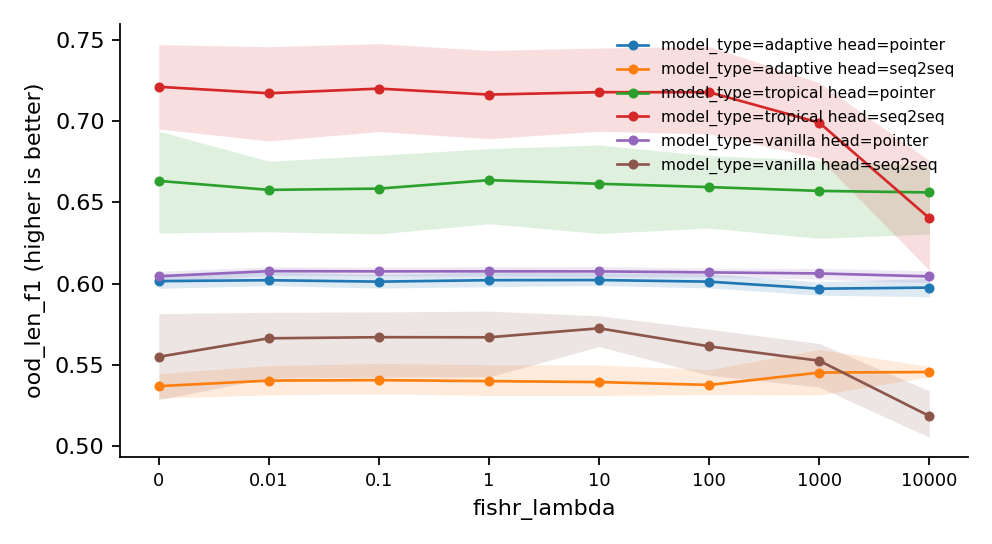
\includegraphics[width=\textwidth]{metric_ood_len_f1.png}
\caption{\texttt{ood\_len\_f1} against \texttt{fishr\_lambda}: the mean over seeds with a 95\% bootstrap CI, one line per combination of the other factors.}
\label{fig:ood_len_f1}
\end{figure}

{\small
\begin{longtable}{lllrlrrr}
\caption{\texttt{ood\_len\_f1} per cell: mean, 95\% bootstrap CI, SD, seeds, diverged runs.}\label{tab:summary-ood_len_f1}\\
\toprule
\texttt{model\_type} & \texttt{head} & \texttt{fishr\_lambda} & mean & 95\% CI & SD & $n$ & div.\\
\midrule
\endhead
adaptive & pointer & 0 & 0.6015 & [0.597, 0.606] & 0.00584 & 5 & 0\\
adaptive & pointer & 0.01 & 0.6021 & [0.599, 0.607] & 0.00551 & 5 & 0\\
adaptive & pointer & 0.1 & 0.6012 & [0.597, 0.606] & 0.00581 & 5 & 0\\
adaptive & pointer & 1 & 0.6021 & [0.598, 0.607] & 0.00606 & 5 & 0\\
adaptive & pointer & 10 & 0.6022 & [0.599, 0.607] & 0.00519 & 5 & 0\\
adaptive & pointer & 100 & 0.6012 & [0.597, 0.606] & 0.00555 & 5 & 0\\
adaptive & pointer & 1000 & 0.5968 & [0.593, 0.601] & 0.00528 & 5 & 0\\
adaptive & pointer & 1e+04 & 0.5975 & [0.592, 0.603] & 0.00713 & 5 & 0\\
adaptive & seq2seq & 0 & 0.5368 & [0.529, 0.544] & 0.0101 & 5 & 0\\
adaptive & seq2seq & 0.01 & 0.5402 & [0.531, 0.549] & 0.0125 & 5 & 0\\
adaptive & seq2seq & 0.1 & 0.5404 & [0.532, 0.551] & 0.0123 & 5 & 0\\
adaptive & seq2seq & 1 & 0.5398 & [0.531, 0.55] & 0.0123 & 5 & 0\\
adaptive & seq2seq & 10 & 0.5392 & [0.531, 0.55] & 0.012 & 5 & 0\\
adaptive & seq2seq & 100 & 0.5375 & [0.531, 0.547] & 0.0103 & 5 & 0\\
adaptive & seq2seq & 1000 & 0.5451 & [0.531, 0.559] & 0.0191 & 5 & 0\\
adaptive & seq2seq & 1e+04 & 0.5454 & [0.542, 0.549] & 0.00402 & 5 & 0\\
tropical & pointer & 0 & 0.6633 & [0.631, 0.694] & 0.0376 & 5 & 0\\
tropical & pointer & 0.01 & 0.6578 & [0.632, 0.675] & 0.0298 & 5 & 0\\
tropical & pointer & 0.1 & 0.6585 & [0.631, 0.679] & 0.0328 & 5 & 0\\
tropical & pointer & 1 & 0.6638 & [0.637, 0.683] & 0.0313 & 5 & 0\\
tropical & pointer & 10 & 0.6615 & [0.631, 0.685] & 0.0368 & 5 & 0\\
tropical & pointer & 100 & 0.6595 & [0.634, 0.679] & 0.0287 & 5 & 0\\
tropical & pointer & 1000 & 0.6571 & [0.628, 0.676] & 0.0326 & 5 & 0\\
tropical & pointer & 1e+04 & 0.6562 & [0.631, 0.672] & 0.0277 & 5 & 0\\
tropical & seq2seq & 0 & 0.7213 & [0.695, 0.747] & 0.033 & 5 & 0\\
tropical & seq2seq & 0.01 & 0.7173 & [0.688, 0.746] & 0.0383 & 5 & 0\\
tropical & seq2seq & 0.1 & 0.7202 & [0.694, 0.748] & 0.0365 & 5 & 0\\
tropical & seq2seq & 1 & 0.7165 & [0.689, 0.744] & 0.0367 & 5 & 0\\
tropical & seq2seq & 10 & 0.718 & [0.694, 0.745] & 0.0327 & 5 & 0\\
tropical & seq2seq & 100 & 0.718 & [0.692, 0.746] & 0.0352 & 5 & 0\\
tropical & seq2seq & 1000 & 0.6992 & [0.677, 0.724] & 0.0312 & 5 & 0\\
tropical & seq2seq & 1e+04 & 0.6402 & [0.608, 0.676] & 0.0435 & 5 & 0\\
vanilla & pointer & 0 & 0.6045 & [0.601, 0.608] & 0.00456 & 5 & 0\\
vanilla & pointer & 0.01 & 0.6076 & [0.605, 0.61] & 0.00354 & 5 & 0\\
vanilla & pointer & 0.1 & 0.6075 & [0.605, 0.61] & 0.00351 & 5 & 0\\
vanilla & pointer & 1 & 0.6075 & [0.605, 0.61] & 0.00379 & 5 & 0\\
vanilla & pointer & 10 & 0.6075 & [0.604, 0.611] & 0.00399 & 5 & 0\\
vanilla & pointer & 100 & 0.6069 & [0.604, 0.609] & 0.00348 & 5 & 0\\
vanilla & pointer & 1000 & 0.6062 & [0.603, 0.609] & 0.00414 & 5 & 0\\
vanilla & pointer & 1e+04 & 0.6044 & [0.6, 0.608] & 0.00476 & 5 & 0\\
vanilla & seq2seq & 0 & 0.5548 & [0.528, 0.581] & 0.0349 & 5 & 0\\
vanilla & seq2seq & 0.01 & 0.5662 & [0.542, 0.582] & 0.0273 & 5 & 0\\
vanilla & seq2seq & 0.1 & 0.5669 & [0.542, 0.583] & 0.0274 & 5 & 0\\
vanilla & seq2seq & 1 & 0.5669 & [0.542, 0.583] & 0.0274 & 5 & 0\\
vanilla & seq2seq & 10 & 0.5724 & [0.561, 0.58] & 0.0123 & 5 & 0\\
vanilla & seq2seq & 100 & 0.5612 & [0.543, 0.572] & 0.0199 & 5 & 0\\
vanilla & seq2seq & 1000 & 0.5524 & [0.536, 0.563] & 0.0183 & 5 & 0\\
vanilla & seq2seq & 1e+04 & 0.5182 & [0.505, 0.534] & 0.0173 & 5 & 0\\
\bottomrule
\end{longtable}
}

{\small
\begin{longtable}{lllrrrl}
\caption{\texttt{ood\_len\_f1}: each level of \texttt{fishr\_lambda} against its control (0), within each combination of the other factors. parametric: Dunnett vs control.}\label{tab:control-ood_len_f1}\\
\toprule
\texttt{model\_type} & \texttt{head} & \texttt{fishr\_lambda} & difference & 95\% CI & $p$ & \\
\midrule
\endhead
adaptive & pointer & 0.01 & $5.591\times10^{-4}$ & [-0.00962, 0.0107] & 1.0000 & \\
adaptive & pointer & 0.1 & $-3.183\times10^{-4}$ & [-0.0105, 0.00986] & 1.0000 & \\
adaptive & pointer & 1 & $5.843\times10^{-4}$ & [-0.00959, 0.0108] & 1.0000 & \\
adaptive & pointer & 10 & $6.681\times10^{-4}$ & [-0.00951, 0.0108] & 1.0000 & \\
adaptive & pointer & 100 & $-3.246\times10^{-4}$ & [-0.0105, 0.00985] & 1.0000 & \\
adaptive & pointer & 1000 & -0.004661 & [-0.0148, 0.00551] & 0.6834 & \\
adaptive & pointer & 1e+04 & -0.003985 & [-0.0142, 0.00619] & 0.8066 & \\
adaptive & seq2seq & 0.01 & 0.003397 & [-0.0179, 0.0247] & 0.9979 & \\
adaptive & seq2seq & 0.1 & 0.003664 & [-0.0177, 0.025] & 0.9966 & \\
adaptive & seq2seq & 1 & 0.003076 & [-0.0183, 0.0244] & 0.9988 & \\
adaptive & seq2seq & 10 & 0.002487 & [-0.0188, 0.0238] & 0.9997 & \\
adaptive & seq2seq & 100 & $7.360\times10^{-4}$ & [-0.0206, 0.0221] & 1.0000 & \\
adaptive & seq2seq & 1000 & 0.008352 & [-0.013, 0.0297] & 0.8067 & \\
adaptive & seq2seq & 1e+04 & 0.008674 & [-0.0127, 0.03] & 0.7804 & \\
tropical & pointer & 0.01 & -0.00556 & [-0.0621, 0.051] & 0.9999 & \\
tropical & pointer & 0.1 & -0.004773 & [-0.0613, 0.0517] & 1.0000 & \\
tropical & pointer & 1 & $4.440\times10^{-4}$ & [-0.0561, 0.057] & 1.0000 & \\
tropical & pointer & 10 & -0.001797 & [-0.0583, 0.0547] & 1.0000 & \\
tropical & pointer & 100 & -0.003838 & [-0.0603, 0.0527] & 1.0000 & \\
tropical & pointer & 1000 & -0.006183 & [-0.0627, 0.0503] & 0.9998 & \\
tropical & pointer & 1e+04 & -0.007141 & [-0.0637, 0.0494] & 0.9995 & \\
tropical & seq2seq & 0.01 & -0.003974 & [-0.067, 0.059] & 1.0000 & \\
tropical & seq2seq & 0.1 & -0.001111 & [-0.0641, 0.0619] & 1.0000 & \\
tropical & seq2seq & 1 & -0.004786 & [-0.0678, 0.0582] & 1.0000 & \\
tropical & seq2seq & 10 & -0.003318 & [-0.0663, 0.0597] & 1.0000 & \\
tropical & seq2seq & 100 & -0.003346 & [-0.0663, 0.0596] & 1.0000 & \\
tropical & seq2seq & 1000 & -0.02216 & [-0.0851, 0.0408] & 0.8697 & \\
tropical & seq2seq & 1e+04 & -0.08108 & [-0.144, -0.0181] & 0.0072 & *\\
vanilla & pointer & 0.01 & 0.00314 & [-0.00384, 0.0101] & 0.6998 & \\
vanilla & pointer & 0.1 & 0.003006 & [-0.00398, 0.00999] & 0.7366 & \\
vanilla & pointer & 1 & 0.003034 & [-0.00395, 0.01] & 0.7287 & \\
vanilla & pointer & 10 & 0.002993 & [-0.00399, 0.00998] & 0.7400 & \\
vanilla & pointer & 100 & 0.002383 & [-0.0046, 0.00937] & 0.8846 & \\
vanilla & pointer & 1000 & 0.001711 & [-0.00527, 0.00869] & 0.9750 & \\
vanilla & pointer & 1e+04 & $-1.009\times10^{-4}$ & [-0.00708, 0.00688] & 1.0000 & \\
vanilla & seq2seq & 0.01 & 0.01141 & [-0.0307, 0.0535] & 0.9585 & \\
vanilla & seq2seq & 0.1 & 0.01209 & [-0.03, 0.0542] & 0.9455 & \\
vanilla & seq2seq & 1 & 0.01202 & [-0.0301, 0.0541] & 0.9469 & \\
vanilla & seq2seq & 10 & 0.01757 & [-0.0245, 0.0597] & 0.7605 & \\
vanilla & seq2seq & 100 & 0.006413 & [-0.0357, 0.0485] & 0.9984 & \\
vanilla & seq2seq & 1000 & -0.002442 & [-0.0445, 0.0396] & 1.0000 & \\
vanilla & seq2seq & 1e+04 & -0.03659 & [-0.0787, 0.0055] & 0.1096 & \\
\bottomrule
\end{longtable}
}

{\small
\begin{longtable}{llrrrrr}
\caption{\texttt{ood\_len\_f1} against log10 \texttt{fishr\_lambda}: parametric: OLS slope t-test, seed-bootstrap CI, with the Jonckheere--Terpstra ordered-trend $\tau$ and $p$.}\label{tab:trend-ood_len_f1}\\
\toprule
\texttt{model\_type} & \texttt{head} & estimate & 95\% CI & $p$ & JT $\tau$ & JT $p$\\
\midrule
\endhead
adaptive & pointer & $-8.295\times10^{-4}$ & [-0.00126, $-2.09\times10^{-4}$] & 0.0850 & -0.2 & 0.1316\\
adaptive & seq2seq & $8.167\times10^{-4}$ & [-0.00129, 0.00262] & 0.4160 & 0.116 & 0.3945\\
tropical & pointer & $-4.231\times10^{-4}$ & [-0.00106, $2.16\times10^{-4}$] & 0.8646 & -0.0438 & 0.7461\\
tropical & seq2seq & -0.009714 & [-0.0123, -0.0073] & 0.0055 & -0.33 & 0.0112\\
vanilla & pointer & $-4.629\times10^{-4}$ & [$-6.89\times10^{-4}$, $-2.37\times10^{-4}$] & 0.1432 & -0.215 & 0.1108\\
vanilla & seq2seq & -0.006381 & [-0.0107, -0.00133] & 0.0030 & -0.478 & 0.0004\\
\bottomrule
\end{longtable}
}

{\small
\begin{longtable}{lrrrl}
\caption{\texttt{ood\_len\_f1}: paired contrasts by seed, Holm-corrected across the cells. parametric: paired t-test by seed, Holm.}\label{tab:paired-ood_len_f1}\\
\toprule
contrast (within) & difference & 95\% CI & $p$ & \\
\midrule
\endhead
\stackcell{model\_type: tropical - vanilla\\\footnotesize head=pointer fishr\_lambda=0 } & 0.05881 & [0.00771, 0.11] & 0.1061 & \\
\stackcell{model\_type: tropical - vanilla\\\footnotesize head=pointer fishr\_lambda=0.01 } & 0.05011 & [0.0138, 0.0865] & 0.1061 & \\
\stackcell{model\_type: tropical - vanilla\\\footnotesize head=pointer fishr\_lambda=0.1 } & 0.05103 & [0.0108, 0.0912] & 0.1061 & \\
\stackcell{model\_type: tropical - vanilla\\\footnotesize head=pointer fishr\_lambda=1 } & 0.05622 & [0.018, 0.0944] & 0.1061 & \\
\stackcell{model\_type: tropical - vanilla\\\footnotesize head=pointer fishr\_lambda=10 } & 0.05402 & [0.00858, 0.0995] & 0.1061 & \\
\stackcell{model\_type: tropical - vanilla\\\footnotesize head=pointer fishr\_lambda=100 } & 0.05259 & [0.017, 0.0882] & 0.1061 & \\
\stackcell{model\_type: tropical - vanilla\\\footnotesize head=pointer fishr\_lambda=1000 } & 0.05092 & [0.0112, 0.0906] & 0.1061 & \\
\stackcell{model\_type: tropical - vanilla\\\footnotesize head=pointer fishr\_lambda=1e+04 } & 0.05177 & [0.0179, 0.0857] & 0.1061 & \\
\stackcell{model\_type: tropical - vanilla\\\footnotesize head=seq2seq fishr\_lambda=0 } & 0.1665 & [0.112, 0.221] & 0.0125 & *\\
\stackcell{model\_type: tropical - vanilla\\\footnotesize head=seq2seq fishr\_lambda=0.01 } & 0.1511 & [0.0995, 0.203] & 0.0125 & *\\
\stackcell{model\_type: tropical - vanilla\\\footnotesize head=seq2seq fishr\_lambda=0.1 } & 0.1533 & [0.104, 0.203] & 0.0125 & *\\
\stackcell{model\_type: tropical - vanilla\\\footnotesize head=seq2seq fishr\_lambda=1 } & 0.1497 & [0.102, 0.197] & 0.0125 & *\\
\stackcell{model\_type: tropical - vanilla\\\footnotesize head=seq2seq fishr\_lambda=10 } & 0.1456 & [0.109, 0.182] & 0.0058 & *\\
\stackcell{model\_type: tropical - vanilla\\\footnotesize head=seq2seq fishr\_lambda=100 } & 0.1567 & [0.118, 0.196] & 0.0058 & *\\
\stackcell{model\_type: tropical - vanilla\\\footnotesize head=seq2seq fishr\_lambda=1000 } & 0.1468 & [0.11, 0.184] & 0.0058 & *\\
\stackcell{model\_type: tropical - vanilla\\\footnotesize head=seq2seq fishr\_lambda=1e+04 } & 0.122 & [0.0719, 0.172] & 0.0224 & *\\
\stackcell{model\_type: adaptive - vanilla\\\footnotesize head=pointer fishr\_lambda=0 } & -0.003014 & [-0.0143, 0.00828] & 1.0000 & \\
\stackcell{model\_type: adaptive - vanilla\\\footnotesize head=pointer fishr\_lambda=0.01 } & -0.005594 & [-0.0154, 0.00419] & 1.0000 & \\
\stackcell{model\_type: adaptive - vanilla\\\footnotesize head=pointer fishr\_lambda=0.1 } & -0.006338 & [-0.0163, 0.00367] & 1.0000 & \\
\stackcell{model\_type: adaptive - vanilla\\\footnotesize head=pointer fishr\_lambda=1 } & -0.005464 & [-0.0163, 0.0054] & 1.0000 & \\
\stackcell{model\_type: adaptive - vanilla\\\footnotesize head=pointer fishr\_lambda=10 } & -0.005338 & [-0.0154, 0.00473] & 1.0000 & \\
\stackcell{model\_type: adaptive - vanilla\\\footnotesize head=pointer fishr\_lambda=100 } & -0.005721 & [-0.0154, 0.004] & 1.0000 & \\
\stackcell{model\_type: adaptive - vanilla\\\footnotesize head=pointer fishr\_lambda=1000 } & -0.009386 & [-0.0173, -0.00149] & 0.4190 & \\
\stackcell{model\_type: adaptive - vanilla\\\footnotesize head=pointer fishr\_lambda=1e+04 } & -0.006897 & [-0.0193, 0.00546] & 1.0000 & \\
\stackcell{model\_type: adaptive - vanilla\\\footnotesize head=seq2seq fishr\_lambda=0 } & -0.01807 & [-0.0644, 0.0283] & 1.0000 & \\
\stackcell{model\_type: adaptive - vanilla\\\footnotesize head=seq2seq fishr\_lambda=0.01 } & -0.02609 & [-0.067, 0.0148] & 1.0000 & \\
\stackcell{model\_type: adaptive - vanilla\\\footnotesize head=seq2seq fishr\_lambda=0.1 } & -0.0265 & [-0.0668, 0.0138] & 1.0000 & \\
\stackcell{model\_type: adaptive - vanilla\\\footnotesize head=seq2seq fishr\_lambda=1 } & -0.02702 & [-0.0684, 0.0143] & 1.0000 & \\
\stackcell{model\_type: adaptive - vanilla\\\footnotesize head=seq2seq fishr\_lambda=10 } & -0.03316 & [-0.0574, -0.00894] & 0.3054 & \\
\stackcell{model\_type: adaptive - vanilla\\\footnotesize head=seq2seq fishr\_lambda=100 } & -0.02375 & [-0.0609, 0.0134] & 1.0000 & \\
\stackcell{model\_type: adaptive - vanilla\\\footnotesize head=seq2seq fishr\_lambda=1000 } & -0.00728 & [-0.0417, 0.0272] & 1.0000 & \\
\stackcell{model\_type: adaptive - vanilla\\\footnotesize head=seq2seq fishr\_lambda=1e+04 } & 0.02719 & [0.0065, 0.0479] & 0.3271 & \\
\stackcell{head: pointer - seq2seq\\\footnotesize model\_type=adaptive fishr\_lambda=0 } & 0.06473 & [0.0488, 0.0807] & 0.0075 & *\\
\stackcell{head: pointer - seq2seq\\\footnotesize model\_type=adaptive fishr\_lambda=0.01 } & 0.0619 & [0.044, 0.0798] & 0.0113 & *\\
\stackcell{head: pointer - seq2seq\\\footnotesize model\_type=adaptive fishr\_lambda=0.1 } & 0.06075 & [0.0445, 0.077] & 0.0098 & *\\
\stackcell{head: pointer - seq2seq\\\footnotesize model\_type=adaptive fishr\_lambda=1 } & 0.06224 & [0.0447, 0.0798] & 0.0108 & *\\
\stackcell{head: pointer - seq2seq\\\footnotesize model\_type=adaptive fishr\_lambda=10 } & 0.06292 & [0.0459, 0.0799] & 0.0098 & *\\
\stackcell{head: pointer - seq2seq\\\footnotesize model\_type=adaptive fishr\_lambda=100 } & 0.06367 & [0.0493, 0.078] & 0.0057 & *\\
\stackcell{head: pointer - seq2seq\\\footnotesize model\_type=adaptive fishr\_lambda=1000 } & 0.05172 & [0.0235, 0.0799] & 0.0916 & \\
\stackcell{head: pointer - seq2seq\\\footnotesize model\_type=adaptive fishr\_lambda=1e+04 } & 0.05208 & [0.0425, 0.0617] & 0.0027 & *\\
\stackcell{head: pointer - seq2seq\\\footnotesize model\_type=tropical fishr\_lambda=0 } & -0.058 & [-0.0853, -0.0307] & 0.0619 & \\
\stackcell{head: pointer - seq2seq\\\footnotesize model\_type=tropical fishr\_lambda=0.01 } & -0.05958 & [-0.107, -0.0126] & 0.1860 & \\
\stackcell{head: pointer - seq2seq\\\footnotesize model\_type=tropical fishr\_lambda=0.1 } & -0.06166 & [-0.106, -0.0168] & 0.1860 & \\
\stackcell{head: pointer - seq2seq\\\footnotesize model\_type=tropical fishr\_lambda=1 } & -0.05277 & [-0.0913, -0.0143] & 0.1860 & \\
\stackcell{head: pointer - seq2seq\\\footnotesize model\_type=tropical fishr\_lambda=10 } & -0.05648 & [-0.0974, -0.0155] & 0.1860 & \\
\stackcell{head: pointer - seq2seq\\\footnotesize model\_type=tropical fishr\_lambda=100 } & -0.05849 & [-0.0959, -0.0211] & 0.1343 & \\
\stackcell{head: pointer - seq2seq\\\footnotesize model\_type=tropical fishr\_lambda=1000 } & -0.04202 & [-0.0761, -0.0079] & 0.1860 & \\
\stackcell{head: pointer - seq2seq\\\footnotesize model\_type=tropical fishr\_lambda=1e+04 } & 0.01594 & [-0.0172, 0.0491] & 0.2524 & \\
\stackcell{head: pointer - seq2seq\\\footnotesize model\_type=vanilla fishr\_lambda=0 } & 0.04967 & [0.00313, 0.0962] & 0.1860 & \\
\stackcell{head: pointer - seq2seq\\\footnotesize model\_type=vanilla fishr\_lambda=0.01 } & 0.0414 & [0.00866, 0.0741] & 0.1860 & \\
\stackcell{head: pointer - seq2seq\\\footnotesize model\_type=vanilla fishr\_lambda=0.1 } & 0.04059 & [0.00794, 0.0732] & 0.1860 & \\
\stackcell{head: pointer - seq2seq\\\footnotesize model\_type=vanilla fishr\_lambda=1 } & 0.04069 & [0.00824, 0.0731] & 0.1860 & \\
\stackcell{head: pointer - seq2seq\\\footnotesize model\_type=vanilla fishr\_lambda=10 } & 0.0351 & [0.0199, 0.0503] & 0.0485 & *\\
\stackcell{head: pointer - seq2seq\\\footnotesize model\_type=vanilla fishr\_lambda=100 } & 0.04564 & [0.0174, 0.0739] & 0.1315 & \\
\stackcell{head: pointer - seq2seq\\\footnotesize model\_type=vanilla fishr\_lambda=1000 } & 0.05383 & [0.0276, 0.0801] & 0.0657 & \\
\stackcell{head: pointer - seq2seq\\\footnotesize model\_type=vanilla fishr\_lambda=1e+04 } & 0.08616 & [0.0655, 0.107] & 0.0070 & *\\
\bottomrule
\end{longtable}
}

\clearpage
\appendix
\section{Other metrics}
\subsection{\texttt{ood\_len\_exact}}
\begin{figure}[tbp]
\centering
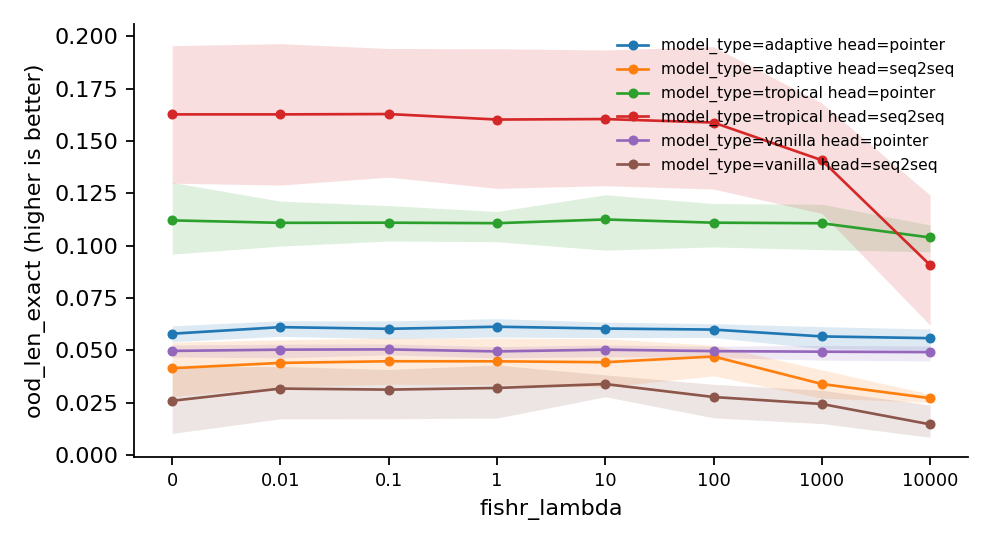
\includegraphics[width=\textwidth]{metric_ood_len_exact.png}
\caption{\texttt{ood\_len\_exact} against \texttt{fishr\_lambda}: the mean over seeds with a 95\% bootstrap CI, one line per combination of the other factors.}
\label{fig:ood_len_exact}
\end{figure}

{\small
\begin{longtable}{lllrlrrr}
\caption{\texttt{ood\_len\_exact} per cell: mean, 95\% bootstrap CI, SD, seeds, diverged runs.}\label{tab:summary-ood_len_exact}\\
\toprule
\texttt{model\_type} & \texttt{head} & \texttt{fishr\_lambda} & mean & 95\% CI & SD & $n$ & div.\\
\midrule
\endhead
adaptive & pointer & 0 & 0.05793 & [0.0541, 0.0617] & 0.00455 & 5 & 0\\
adaptive & pointer & 0.01 & 0.06107 & [0.0567, 0.0641] & 0.00502 & 5 & 0\\
adaptive & pointer & 0.1 & 0.06027 & [0.0555, 0.064] & 0.00545 & 5 & 0\\
adaptive & pointer & 1 & 0.06127 & [0.0563, 0.0651] & 0.00556 & 5 & 0\\
adaptive & pointer & 10 & 0.0604 & [0.0561, 0.0635] & 0.00498 & 5 & 0\\
adaptive & pointer & 100 & 0.0599 & [0.0561, 0.0627] & 0.00439 & 5 & 0\\
adaptive & pointer & 1000 & 0.05663 & [0.0508, 0.0613] & 0.00689 & 5 & 0\\
adaptive & pointer & 1e+04 & 0.0558 & [0.0501, 0.0602] & 0.00675 & 5 & 0\\
adaptive & seq2seq & 0 & 0.04143 & [0.0278, 0.0538] & 0.0166 & 5 & 0\\
adaptive & seq2seq & 0.01 & 0.04397 & [0.0325, 0.055] & 0.0148 & 5 & 0\\
adaptive & seq2seq & 0.1 & 0.04477 & [0.0337, 0.0558] & 0.0148 & 5 & 0\\
adaptive & seq2seq & 1 & 0.04473 & [0.0336, 0.0558] & 0.0148 & 5 & 0\\
adaptive & seq2seq & 10 & 0.0443 & [0.0325, 0.0555] & 0.0154 & 5 & 0\\
adaptive & seq2seq & 100 & 0.04703 & [0.0378, 0.0524] & 0.0103 & 5 & 0\\
adaptive & seq2seq & 1000 & 0.0339 & [0.0271, 0.0407] & 0.00873 & 5 & 0\\
adaptive & seq2seq & 1e+04 & 0.0271 & [0.025, 0.029] & 0.00269 & 5 & 0\\
tropical & pointer & 0 & 0.1121 & [0.096, 0.13] & 0.0213 & 5 & 0\\
tropical & pointer & 0.01 & 0.1109 & [0.0998, 0.121] & 0.0149 & 5 & 0\\
tropical & pointer & 0.1 & 0.111 & [0.102, 0.119] & 0.0113 & 5 & 0\\
tropical & pointer & 1 & 0.1108 & [0.102, 0.116] & 0.00985 & 5 & 0\\
tropical & pointer & 10 & 0.1125 & [0.0979, 0.124] & 0.0176 & 5 & 0\\
tropical & pointer & 100 & 0.111 & [0.0994, 0.12] & 0.0133 & 5 & 0\\
tropical & pointer & 1000 & 0.1107 & [0.0981, 0.12] & 0.0142 & 5 & 0\\
tropical & pointer & 1e+04 & 0.1039 & [0.0971, 0.11] & 0.00833 & 5 & 0\\
tropical & seq2seq & 0 & 0.1628 & [0.13, 0.196] & 0.0418 & 5 & 0\\
tropical & seq2seq & 0.01 & 0.1628 & [0.129, 0.197] & 0.044 & 5 & 0\\
tropical & seq2seq & 0.1 & 0.1629 & [0.133, 0.194] & 0.0411 & 5 & 0\\
tropical & seq2seq & 1 & 0.1603 & [0.127, 0.194] & 0.0451 & 5 & 0\\
tropical & seq2seq & 10 & 0.1605 & [0.129, 0.194] & 0.0416 & 5 & 0\\
tropical & seq2seq & 100 & 0.1589 & [0.127, 0.195] & 0.0432 & 5 & 0\\
tropical & seq2seq & 1000 & 0.1409 & [0.115, 0.168] & 0.035 & 5 & 0\\
tropical & seq2seq & 1e+04 & 0.09073 & [0.062, 0.124] & 0.039 & 5 & 0\\
vanilla & pointer & 0 & 0.0497 & [0.0468, 0.0526] & 0.00374 & 5 & 0\\
vanilla & pointer & 0.01 & 0.0503 & [0.0464, 0.0529] & 0.00437 & 5 & 0\\
vanilla & pointer & 0.1 & 0.05043 & [0.0478, 0.0531] & 0.00357 & 5 & 0\\
vanilla & pointer & 1 & 0.04947 & [0.0464, 0.0517] & 0.00362 & 5 & 0\\
vanilla & pointer & 10 & 0.0503 & [0.047, 0.0526] & 0.00375 & 5 & 0\\
vanilla & pointer & 100 & 0.0496 & [0.0466, 0.0519] & 0.00344 & 5 & 0\\
vanilla & pointer & 1000 & 0.04933 & [0.0453, 0.0523] & 0.00439 & 5 & 0\\
vanilla & pointer & 1e+04 & 0.04913 & [0.0449, 0.0521] & 0.00461 & 5 & 0\\
vanilla & seq2seq & 0 & 0.02587 & [0.0103, 0.042] & 0.0206 & 5 & 0\\
vanilla & seq2seq & 0.01 & 0.0317 & [0.0172, 0.0423] & 0.0164 & 5 & 0\\
vanilla & seq2seq & 0.1 & 0.0312 & [0.0173, 0.0408] & 0.0157 & 5 & 0\\
vanilla & seq2seq & 1 & 0.032 & [0.0176, 0.0429] & 0.017 & 5 & 0\\
vanilla & seq2seq & 10 & 0.03387 & [0.0278, 0.0382] & 0.00699 & 5 & 0\\
vanilla & seq2seq & 100 & 0.02767 & [0.0177, 0.0337] & 0.0112 & 5 & 0\\
vanilla & seq2seq & 1000 & 0.02433 & [0.015, 0.0309] & 0.0104 & 5 & 0\\
vanilla & seq2seq & 1e+04 & 0.0146 & [0.00843, 0.0239] & 0.00957 & 5 & 0\\
\bottomrule
\end{longtable}
}

{\small
\begin{longtable}{lllrrrl}
\caption{\texttt{ood\_len\_exact}: each level of \texttt{fishr\_lambda} against its control (0), within each combination of the other factors. parametric: Dunnett vs control.}\label{tab:control-ood_len_exact}\\
\toprule
\texttt{model\_type} & \texttt{head} & \texttt{fishr\_lambda} & difference & 95\% CI & $p$ & \\
\midrule
\endhead
adaptive & pointer & 0.01 & 0.003133 & [-0.00651, 0.0128] & 0.9054 & \\
adaptive & pointer & 0.1 & 0.002333 & [-0.00731, 0.012] & 0.9766 & \\
adaptive & pointer & 1 & 0.003333 & [-0.00631, 0.013] & 0.8782 & \\
adaptive & pointer & 10 & 0.002467 & [-0.00717, 0.0121] & 0.9688 & \\
adaptive & pointer & 100 & 0.001967 & [-0.00767, 0.0116] & 0.9907 & \\
adaptive & pointer & 1000 & -0.0013 & [-0.0109, 0.00834] & 0.9992 & \\
adaptive & pointer & 1e+04 & -0.002133 & [-0.0118, 0.00751] & 0.9855 & \\
adaptive & seq2seq & 0.01 & 0.002533 & [-0.0202, 0.0253] & 0.9998 & \\
adaptive & seq2seq & 0.1 & 0.003333 & [-0.0194, 0.0261] & 0.9987 & \\
adaptive & seq2seq & 1 & 0.0033 & [-0.0194, 0.026] & 0.9988 & \\
adaptive & seq2seq & 10 & 0.002867 & [-0.0199, 0.0256] & 0.9995 & \\
adaptive & seq2seq & 100 & 0.0056 & [-0.0171, 0.0283] & 0.9744 & \\
adaptive & seq2seq & 1000 & -0.007533 & [-0.0303, 0.0152] & 0.8978 & \\
adaptive & seq2seq & 1e+04 & -0.01433 & [-0.0371, 0.00841] & 0.3664 & \\
tropical & pointer & 0.01 & -0.001167 & [-0.0263, 0.024] & 1.0000 & \\
tropical & pointer & 0.1 & -0.0011 & [-0.0262, 0.024] & 1.0000 & \\
tropical & pointer & 1 & -0.001333 & [-0.0265, 0.0238] & 1.0000 & \\
tropical & pointer & 10 & $4.333\times10^{-4}$ & [-0.0247, 0.0256] & 1.0000 & \\
tropical & pointer & 100 & -0.0011 & [-0.0262, 0.024] & 1.0000 & \\
tropical & pointer & 1000 & -0.001367 & [-0.0265, 0.0238] & 1.0000 & \\
tropical & pointer & 1e+04 & -0.008167 & [-0.0333, 0.017] & 0.9057 & \\
tropical & seq2seq & 0.01 & 0 & [-0.0724, 0.0724] & 1.0000 & \\
tropical & seq2seq & 0.1 & $1.667\times10^{-4}$ & [-0.0722, 0.0726] & 1.0000 & \\
tropical & seq2seq & 1 & -0.002467 & [-0.0749, 0.0699] & 1.0000 & \\
tropical & seq2seq & 10 & -0.002233 & [-0.0746, 0.0702] & 1.0000 & \\
tropical & seq2seq & 100 & -0.0039 & [-0.0763, 0.0685] & 1.0000 & \\
tropical & seq2seq & 1000 & -0.0219 & [-0.0943, 0.0505] & 0.9309 & \\
tropical & seq2seq & 1e+04 & -0.07203 & [-0.144, $3.73\times10^{-4}$] & 0.0517 & \\
vanilla & pointer & 0.01 & $6.000\times10^{-4}$ & [-0.00631, 0.00751] & 1.0000 & \\
vanilla & pointer & 0.1 & $7.333\times10^{-4}$ & [-0.00618, 0.00765] & 0.9998 & \\
vanilla & pointer & 1 & $-2.333\times10^{-4}$ & [-0.00715, 0.00668] & 1.0000 & \\
vanilla & pointer & 10 & $6.000\times10^{-4}$ & [-0.00631, 0.00751] & 1.0000 & \\
vanilla & pointer & 100 & $-1.000\times10^{-4}$ & [-0.00701, 0.00681] & 1.0000 & \\
vanilla & pointer & 1000 & $-3.667\times10^{-4}$ & [-0.00728, 0.00655] & 1.0000 & \\
vanilla & pointer & 1e+04 & $-5.667\times10^{-4}$ & [-0.00748, 0.00635] & 1.0000 & \\
vanilla & seq2seq & 0.01 & 0.005833 & [-0.0189, 0.0306] & 0.9796 & \\
vanilla & seq2seq & 0.1 & 0.005333 & [-0.0194, 0.0301] & 0.9874 & \\
vanilla & seq2seq & 1 & 0.006133 & [-0.0186, 0.0309] & 0.9735 & \\
vanilla & seq2seq & 10 & 0.008 & [-0.0167, 0.0327] & 0.9077 & \\
vanilla & seq2seq & 100 & 0.0018 & [-0.0229, 0.0265] & 1.0000 & \\
vanilla & seq2seq & 1000 & -0.001533 & [-0.0263, 0.0232] & 1.0000 & \\
vanilla & seq2seq & 1e+04 & -0.01127 & [-0.036, 0.0135] & 0.6890 & \\
\bottomrule
\end{longtable}
}

{\small
\begin{longtable}{llrrrrr}
\caption{\texttt{ood\_len\_exact} against log10 \texttt{fishr\_lambda}: parametric: OLS slope t-test, seed-bootstrap CI, with the Jonckheere--Terpstra ordered-trend $\tau$ and $p$.}\label{tab:trend-ood_len_exact}\\
\toprule
\texttt{model\_type} & \texttt{head} & estimate & 95\% CI & $p$ & JT $\tau$ & JT $p$\\
\midrule
\endhead
adaptive & pointer & $-8.726\times10^{-4}$ & [-0.0012, $-4.75\times10^{-4}$] & 0.0603 & -0.29 & 0.0284\\
adaptive & seq2seq & -0.002501 & [-0.00441, $-5.06\times10^{-4}$] & 0.0231 & -0.356 & 0.0078\\
tropical & pointer & $-7.607\times10^{-4}$ & [-0.00167, $2.61\times10^{-4}$] & 0.4682 & -0.133 & 0.3287\\
tropical & seq2seq & -0.009345 & [-0.0112, -0.00751] & 0.0118 & -0.331 & 0.0114\\
vanilla & pointer & $-1.988\times10^{-4}$ & [$-4.86\times10^{-4}$, $1.42\times10^{-4}$] & 0.5278 & -0.131 & 0.3335\\
vanilla & seq2seq & -0.002477 & [-0.00479, $3.68\times10^{-4}$] & 0.0258 & -0.4 & 0.0022\\
\bottomrule
\end{longtable}
}

{\small
\begin{longtable}{lrrrl}
\caption{\texttt{ood\_len\_exact}: paired contrasts by seed, Holm-corrected across the cells. parametric: paired t-test by seed, Holm.}\label{tab:paired-ood_len_exact}\\
\toprule
contrast (within) & difference & 95\% CI & $p$ & \\
\midrule
\endhead
\stackcell{model\_type: tropical - vanilla\\\footnotesize head=pointer fishr\_lambda=0 } & 0.0624 & [0.0377, 0.0871] & 0.0133 & *\\
\stackcell{model\_type: tropical - vanilla\\\footnotesize head=pointer fishr\_lambda=0.01 } & 0.06063 & [0.0468, 0.0744] & 0.0028 & *\\
\stackcell{model\_type: tropical - vanilla\\\footnotesize head=pointer fishr\_lambda=0.1 } & 0.06057 & [0.0493, 0.0718] & 0.0016 & *\\
\stackcell{model\_type: tropical - vanilla\\\footnotesize head=pointer fishr\_lambda=1 } & 0.0613 & [0.0529, 0.0697] & 0.0005 & *\\
\stackcell{model\_type: tropical - vanilla\\\footnotesize head=pointer fishr\_lambda=10 } & 0.06223 & [0.0442, 0.0803] & 0.0067 & *\\
\stackcell{model\_type: tropical - vanilla\\\footnotesize head=pointer fishr\_lambda=100 } & 0.0614 & [0.0485, 0.0743] & 0.0025 & *\\
\stackcell{model\_type: tropical - vanilla\\\footnotesize head=pointer fishr\_lambda=1000 } & 0.0614 & [0.0482, 0.0746] & 0.0025 & *\\
\stackcell{model\_type: tropical - vanilla\\\footnotesize head=pointer fishr\_lambda=1e+04 } & 0.0548 & [0.0488, 0.0608] & 0.0002 & *\\
\stackcell{model\_type: tropical - vanilla\\\footnotesize head=seq2seq fishr\_lambda=0 } & 0.1369 & [0.0826, 0.191] & 0.0133 & *\\
\stackcell{model\_type: tropical - vanilla\\\footnotesize head=seq2seq fishr\_lambda=0.01 } & 0.1311 & [0.0767, 0.185] & 0.0133 & *\\
\stackcell{model\_type: tropical - vanilla\\\footnotesize head=seq2seq fishr\_lambda=0.1 } & 0.1317 & [0.0814, 0.182] & 0.0133 & *\\
\stackcell{model\_type: tropical - vanilla\\\footnotesize head=seq2seq fishr\_lambda=1 } & 0.1283 & [0.0726, 0.184] & 0.0133 & *\\
\stackcell{model\_type: tropical - vanilla\\\footnotesize head=seq2seq fishr\_lambda=10 } & 0.1267 & [0.0772, 0.176] & 0.0133 & *\\
\stackcell{model\_type: tropical - vanilla\\\footnotesize head=seq2seq fishr\_lambda=100 } & 0.1312 & [0.0834, 0.179] & 0.0127 & *\\
\stackcell{model\_type: tropical - vanilla\\\footnotesize head=seq2seq fishr\_lambda=1000 } & 0.1165 & [0.0762, 0.157] & 0.0118 & *\\
\stackcell{model\_type: tropical - vanilla\\\footnotesize head=seq2seq fishr\_lambda=1e+04 } & 0.07613 & [0.0266, 0.126] & 0.0133 & *\\
\stackcell{model\_type: adaptive - vanilla\\\footnotesize head=pointer fishr\_lambda=0 } & 0.008233 & [0.00429, 0.0122] & 0.0439 & *\\
\stackcell{model\_type: adaptive - vanilla\\\footnotesize head=pointer fishr\_lambda=0.01 } & 0.01077 & [0.00941, 0.0121] & 0.0004 & *\\
\stackcell{model\_type: adaptive - vanilla\\\footnotesize head=pointer fishr\_lambda=0.1 } & 0.009833 & [0.00735, 0.0123] & 0.0047 & *\\
\stackcell{model\_type: adaptive - vanilla\\\footnotesize head=pointer fishr\_lambda=1 } & 0.0118 & [0.00862, 0.015] & 0.0055 & *\\
\stackcell{model\_type: adaptive - vanilla\\\footnotesize head=pointer fishr\_lambda=10 } & 0.0101 & [0.008, 0.0122] & 0.0024 & *\\
\stackcell{model\_type: adaptive - vanilla\\\footnotesize head=pointer fishr\_lambda=100 } & 0.0103 & [0.00831, 0.0123] & 0.0019 & *\\
\stackcell{model\_type: adaptive - vanilla\\\footnotesize head=pointer fishr\_lambda=1000 } & 0.0073 & [0.00319, 0.0114] & 0.0627 & \\
\stackcell{model\_type: adaptive - vanilla\\\footnotesize head=pointer fishr\_lambda=1e+04 } & 0.006667 & [0.00343, 0.00991] & 0.0439 & *\\
\stackcell{model\_type: adaptive - vanilla\\\footnotesize head=seq2seq fishr\_lambda=0 } & 0.01557 & [-0.0115, 0.0426] & 0.5327 & \\
\stackcell{model\_type: adaptive - vanilla\\\footnotesize head=seq2seq fishr\_lambda=0.01 } & 0.01227 & [-0.00513, 0.0297] & 0.5327 & \\
\stackcell{model\_type: adaptive - vanilla\\\footnotesize head=seq2seq fishr\_lambda=0.1 } & 0.01357 & [-0.00199, 0.0291] & 0.4362 & \\
\stackcell{model\_type: adaptive - vanilla\\\footnotesize head=seq2seq fishr\_lambda=1 } & 0.01273 & [-0.0043, 0.0298] & 0.5327 & \\
\stackcell{model\_type: adaptive - vanilla\\\footnotesize head=seq2seq fishr\_lambda=10 } & 0.01043 & [-0.00365, 0.0245] & 0.5327 & \\
\stackcell{model\_type: adaptive - vanilla\\\footnotesize head=seq2seq fishr\_lambda=100 } & 0.01937 & [0.0177, 0.0211] & $<10^{-4}$ & *\\
\stackcell{model\_type: adaptive - vanilla\\\footnotesize head=seq2seq fishr\_lambda=1000 } & 0.009567 & [-0.00401, 0.0231] & 0.5327 & \\
\stackcell{model\_type: adaptive - vanilla\\\footnotesize head=seq2seq fishr\_lambda=1e+04 } & 0.0125 & [0.00334, 0.0217] & 0.1349 & \\
\stackcell{head: pointer - seq2seq\\\footnotesize model\_type=adaptive fishr\_lambda=0 } & 0.0165 & [-0.00253, 0.0355] & 0.5792 & \\
\stackcell{head: pointer - seq2seq\\\footnotesize model\_type=adaptive fishr\_lambda=0.01 } & 0.0171 & [0.00108, 0.0331] & 0.5792 & \\
\stackcell{head: pointer - seq2seq\\\footnotesize model\_type=adaptive fishr\_lambda=0.1 } & 0.0155 & [$-8.76\times10^{-4}$, 0.0319] & 0.5792 & \\
\stackcell{head: pointer - seq2seq\\\footnotesize model\_type=adaptive fishr\_lambda=1 } & 0.01653 & [$3.61\times10^{-4}$, 0.0327] & 0.5792 & \\
\stackcell{head: pointer - seq2seq\\\footnotesize model\_type=adaptive fishr\_lambda=10 } & 0.0161 & [$-4.84\times10^{-6}$, 0.0322] & 0.5792 & \\
\stackcell{head: pointer - seq2seq\\\footnotesize model\_type=adaptive fishr\_lambda=100 } & 0.01287 & [-0.00257, 0.0283] & 0.5792 & \\
\stackcell{head: pointer - seq2seq\\\footnotesize model\_type=adaptive fishr\_lambda=1000 } & 0.02273 & [0.0094, 0.0361] & 0.1814 & \\
\stackcell{head: pointer - seq2seq\\\footnotesize model\_type=adaptive fishr\_lambda=1e+04 } & 0.0287 & [0.0203, 0.0371] & 0.0166 & *\\
\stackcell{head: pointer - seq2seq\\\footnotesize model\_type=tropical fishr\_lambda=0 } & -0.05067 & [-0.0846, -0.0167] & 0.2731 & \\
\stackcell{head: pointer - seq2seq\\\footnotesize model\_type=tropical fishr\_lambda=0.01 } & -0.05183 & [-0.104, $5.94\times10^{-4}$] & 0.5792 & \\
\stackcell{head: pointer - seq2seq\\\footnotesize model\_type=tropical fishr\_lambda=0.1 } & -0.05193 & [-0.102, -0.00167] & 0.5792 & \\
\stackcell{head: pointer - seq2seq\\\footnotesize model\_type=tropical fishr\_lambda=1 } & -0.04953 & [-0.101, 0.00168] & 0.5792 & \\
\stackcell{head: pointer - seq2seq\\\footnotesize model\_type=tropical fishr\_lambda=10 } & -0.048 & [-0.0917, -0.00434] & 0.5691 & \\
\stackcell{head: pointer - seq2seq\\\footnotesize model\_type=tropical fishr\_lambda=100 } & -0.04787 & [-0.0928, -0.00291] & 0.5792 & \\
\stackcell{head: pointer - seq2seq\\\footnotesize model\_type=tropical fishr\_lambda=1000 } & -0.03013 & [-0.0661, 0.00585] & 0.5792 & \\
\stackcell{head: pointer - seq2seq\\\footnotesize model\_type=tropical fishr\_lambda=1e+04 } & 0.0132 & [-0.0337, 0.0601] & 0.5792 & \\
\stackcell{head: pointer - seq2seq\\\footnotesize model\_type=vanilla fishr\_lambda=0 } & 0.02383 & [-0.00208, 0.0497] & 0.5792 & \\
\stackcell{head: pointer - seq2seq\\\footnotesize model\_type=vanilla fishr\_lambda=0.01 } & 0.0186 & [0.00312, 0.0341] & 0.4923 & \\
\stackcell{head: pointer - seq2seq\\\footnotesize model\_type=vanilla fishr\_lambda=0.1 } & 0.01923 & [0.0028, 0.0357] & 0.5021 & \\
\stackcell{head: pointer - seq2seq\\\footnotesize model\_type=vanilla fishr\_lambda=1 } & 0.01747 & [$-5.43\times10^{-5}$, 0.035] & 0.5792 & \\
\stackcell{head: pointer - seq2seq\\\footnotesize model\_type=vanilla fishr\_lambda=10 } & 0.01643 & [0.0111, 0.0218] & 0.0234 & *\\
\stackcell{head: pointer - seq2seq\\\footnotesize model\_type=vanilla fishr\_lambda=100 } & 0.02193 & [0.00598, 0.0379] & 0.3389 & \\
\stackcell{head: pointer - seq2seq\\\footnotesize model\_type=vanilla fishr\_lambda=1000 } & 0.025 & [0.0108, 0.0392] & 0.1695 & \\
\stackcell{head: pointer - seq2seq\\\footnotesize model\_type=vanilla fishr\_lambda=1e+04 } & 0.03453 & [0.0233, 0.0458] & 0.0234 & *\\
\bottomrule
\end{longtable}
}

\subsection{\texttt{ood\_val\_f1}}
\begin{figure}[tbp]
\centering
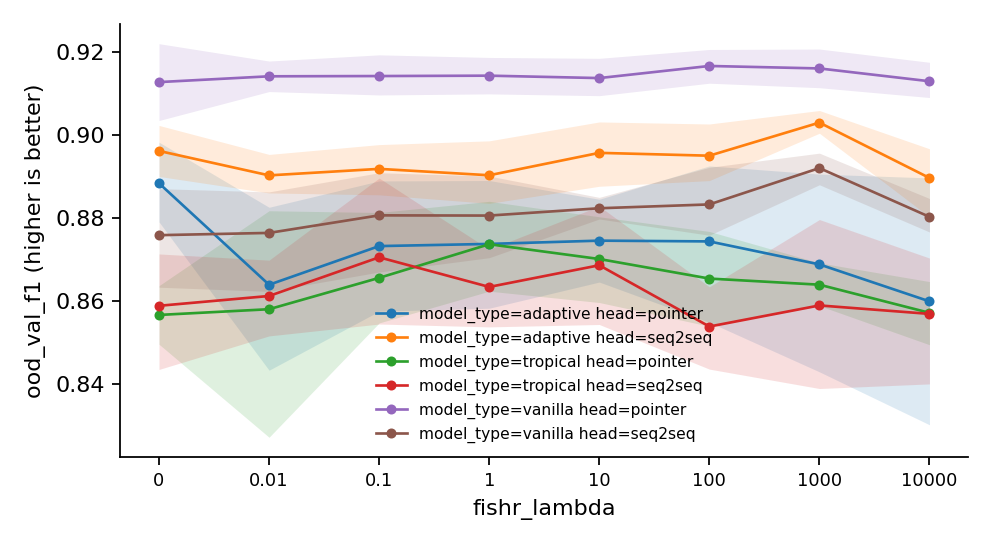
\includegraphics[width=\textwidth]{metric_ood_val_f1.png}
\caption{\texttt{ood\_val\_f1} against \texttt{fishr\_lambda}: the mean over seeds with a 95\% bootstrap CI, one line per combination of the other factors.}
\label{fig:ood_val_f1}
\end{figure}

{\small
\begin{longtable}{lllrlrrr}
\caption{\texttt{ood\_val\_f1} per cell: mean, 95\% bootstrap CI, SD, seeds, diverged runs.}\label{tab:summary-ood_val_f1}\\
\toprule
\texttt{model\_type} & \texttt{head} & \texttt{fishr\_lambda} & mean & 95\% CI & SD & $n$ & div.\\
\midrule
\endhead
adaptive & pointer & 0 & 0.8884 & [0.879, 0.898] & 0.0126 & 5 & 0\\
adaptive & pointer & 0.01 & 0.8639 & [0.843, 0.883] & 0.0241 & 5 & 0\\
adaptive & pointer & 0.1 & 0.8732 & [0.858, 0.889] & 0.02 & 5 & 0\\
adaptive & pointer & 1 & 0.8738 & [0.858, 0.889] & 0.0199 & 5 & 0\\
adaptive & pointer & 10 & 0.8746 & [0.865, 0.885] & 0.0132 & 5 & 0\\
adaptive & pointer & 100 & 0.8744 & [0.855, 0.893] & 0.0243 & 5 & 0\\
adaptive & pointer & 1000 & 0.8688 & [0.843, 0.891] & 0.0311 & 5 & 0\\
adaptive & pointer & 1e+04 & 0.8599 & [0.83, 0.89] & 0.0396 & 5 & 0\\
adaptive & seq2seq & 0 & 0.8962 & [0.89, 0.902] & 0.00793 & 5 & 0\\
adaptive & seq2seq & 0.01 & 0.8903 & [0.886, 0.895] & 0.00631 & 5 & 0\\
adaptive & seq2seq & 0.1 & 0.8918 & [0.886, 0.898] & 0.00797 & 5 & 0\\
adaptive & seq2seq & 1 & 0.8903 & [0.884, 0.899] & 0.0097 & 5 & 0\\
adaptive & seq2seq & 10 & 0.8957 & [0.888, 0.903] & 0.0105 & 5 & 0\\
adaptive & seq2seq & 100 & 0.895 & [0.889, 0.903] & 0.00852 & 5 & 0\\
adaptive & seq2seq & 1000 & 0.903 & [0.9, 0.906] & 0.0034 & 5 & 0\\
adaptive & seq2seq & 1e+04 & 0.8897 & [0.88, 0.897] & 0.0106 & 5 & 0\\
tropical & pointer & 0 & 0.8567 & [0.85, 0.864] & 0.00937 & 5 & 0\\
tropical & pointer & 0.01 & 0.858 & [0.827, 0.882] & 0.036 & 5 & 0\\
tropical & pointer & 0.1 & 0.8656 & [0.855, 0.881] & 0.0179 & 5 & 0\\
tropical & pointer & 1 & 0.8737 & [0.862, 0.884] & 0.0133 & 5 & 0\\
tropical & pointer & 10 & 0.8701 & [0.86, 0.88] & 0.0134 & 5 & 0\\
tropical & pointer & 100 & 0.8654 & [0.854, 0.877] & 0.0149 & 5 & 0\\
tropical & pointer & 1000 & 0.8639 & [0.859, 0.869] & 0.00631 & 5 & 0\\
tropical & pointer & 1e+04 & 0.8572 & [0.849, 0.865] & 0.0106 & 5 & 0\\
tropical & seq2seq & 0 & 0.8589 & [0.844, 0.871] & 0.0169 & 5 & 0\\
tropical & seq2seq & 0.01 & 0.8612 & [0.852, 0.87] & 0.012 & 5 & 0\\
tropical & seq2seq & 0.1 & 0.8705 & [0.854, 0.89] & 0.0221 & 5 & 0\\
tropical & seq2seq & 1 & 0.8634 & [0.854, 0.872] & 0.0119 & 5 & 0\\
tropical & seq2seq & 10 & 0.8686 & [0.854, 0.883] & 0.0186 & 5 & 0\\
tropical & seq2seq & 100 & 0.8539 & [0.844, 0.863] & 0.0128 & 5 & 0\\
tropical & seq2seq & 1000 & 0.8589 & [0.839, 0.88] & 0.0279 & 5 & 0\\
tropical & seq2seq & 1e+04 & 0.8569 & [0.84, 0.87] & 0.0208 & 5 & 0\\
vanilla & pointer & 0 & 0.9127 & [0.903, 0.922] & 0.0116 & 5 & 0\\
vanilla & pointer & 0.01 & 0.9141 & [0.91, 0.918] & 0.00472 & 5 & 0\\
vanilla & pointer & 0.1 & 0.9142 & [0.91, 0.919] & 0.00658 & 5 & 0\\
vanilla & pointer & 1 & 0.9143 & [0.91, 0.919] & 0.00552 & 5 & 0\\
vanilla & pointer & 10 & 0.9137 & [0.909, 0.918] & 0.00587 & 5 & 0\\
vanilla & pointer & 100 & 0.9166 & [0.912, 0.921] & 0.00546 & 5 & 0\\
vanilla & pointer & 1000 & 0.916 & [0.911, 0.921] & 0.00616 & 5 & 0\\
vanilla & pointer & 1e+04 & 0.9129 & [0.909, 0.918] & 0.00536 & 5 & 0\\
vanilla & seq2seq & 0 & 0.8759 & [0.863, 0.887] & 0.0154 & 5 & 0\\
vanilla & seq2seq & 0.01 & 0.8764 & [0.862, 0.886] & 0.0164 & 5 & 0\\
vanilla & seq2seq & 0.1 & 0.8806 & [0.867, 0.891] & 0.016 & 5 & 0\\
vanilla & seq2seq & 1 & 0.8806 & [0.87, 0.89] & 0.0125 & 5 & 0\\
vanilla & seq2seq & 10 & 0.8824 & [0.88, 0.885] & 0.00336 & 5 & 0\\
vanilla & seq2seq & 100 & 0.8833 & [0.876, 0.892] & 0.0109 & 5 & 0\\
vanilla & seq2seq & 1000 & 0.892 & [0.888, 0.896] & 0.00471 & 5 & 0\\
vanilla & seq2seq & 1e+04 & 0.8803 & [0.877, 0.885] & 0.00528 & 5 & 0\\
\bottomrule
\end{longtable}
}

{\small
\begin{longtable}{lllrrrl}
\caption{\texttt{ood\_val\_f1}: each level of \texttt{fishr\_lambda} against its control (0), within each combination of the other factors. parametric: Dunnett vs control.}\label{tab:control-ood_val_f1}\\
\toprule
\texttt{model\_type} & \texttt{head} & \texttt{fishr\_lambda} & difference & 95\% CI & $p$ & \\
\midrule
\endhead
adaptive & pointer & 0.01 & -0.02445 & [-0.0674, 0.0185] & 0.4698 & \\
adaptive & pointer & 0.1 & -0.01513 & [-0.0581, 0.0278] & 0.8688 & \\
adaptive & pointer & 1 & -0.01461 & [-0.0576, 0.0283] & 0.8859 & \\
adaptive & pointer & 10 & -0.01383 & [-0.0568, 0.0291] & 0.9092 & \\
adaptive & pointer & 100 & -0.01401 & [-0.057, 0.0289] & 0.9040 & \\
adaptive & pointer & 1000 & -0.01954 & [-0.0625, 0.0234] & 0.6891 & \\
adaptive & pointer & 1e+04 & -0.02844 & [-0.0714, 0.0145] & 0.3177 & \\
adaptive & seq2seq & 0.01 & -0.005887 & [-0.0206, 0.00882] & 0.7915 & \\
adaptive & seq2seq & 0.1 & -0.00432 & [-0.019, 0.0104] & 0.9395 & \\
adaptive & seq2seq & 1 & -0.005859 & [-0.0206, 0.00885] & 0.7948 & \\
adaptive & seq2seq & 10 & $-4.641\times10^{-4}$ & [-0.0152, 0.0142] & 1.0000 & \\
adaptive & seq2seq & 100 & -0.001148 & [-0.0159, 0.0136] & 1.0000 & \\
adaptive & seq2seq & 1000 & 0.006824 & [-0.00788, 0.0215] & 0.6719 & \\
adaptive & seq2seq & 1e+04 & -0.006506 & [-0.0212, 0.0082] & 0.7139 & \\
tropical & pointer & 0.01 & 0.00138 & [-0.0291, 0.0318] & 1.0000 & \\
tropical & pointer & 0.1 & 0.008931 & [-0.0215, 0.0394] & 0.9399 & \\
tropical & pointer & 1 & 0.01703 & [-0.0134, 0.0475] & 0.4881 & \\
tropical & pointer & 10 & 0.01347 & [-0.017, 0.0439] & 0.7136 & \\
tropical & pointer & 100 & 0.00876 & [-0.0217, 0.0392] & 0.9450 & \\
tropical & pointer & 1000 & 0.007287 & [-0.0232, 0.0377] & 0.9779 & \\
tropical & pointer & 1e+04 & $5.125\times10^{-4}$ & [-0.0299, 0.031] & 1.0000 & \\
tropical & seq2seq & 0.01 & 0.002364 & [-0.0302, 0.0349] & 1.0000 & \\
tropical & seq2seq & 0.1 & 0.01168 & [-0.0209, 0.0443] & 0.8598 & \\
tropical & seq2seq & 1 & 0.004544 & [-0.028, 0.0371] & 0.9991 & \\
tropical & seq2seq & 10 & 0.009766 & [-0.0228, 0.0423] & 0.9336 & \\
tropical & seq2seq & 100 & -0.004994 & [-0.0376, 0.0276] & 0.9983 & \\
tropical & seq2seq & 1000 & $8.736\times10^{-5}$ & [-0.0325, 0.0327] & 1.0000 & \\
tropical & seq2seq & 1e+04 & -0.001948 & [-0.0345, 0.0306] & 1.0000 & \\
vanilla & pointer & 0.01 & 0.001394 & [-0.0104, 0.0132] & 0.9997 & \\
vanilla & pointer & 0.1 & 0.001457 & [-0.0103, 0.0132] & 0.9996 & \\
vanilla & pointer & 1 & 0.001548 & [-0.0102, 0.0133] & 0.9993 & \\
vanilla & pointer & 10 & $9.674\times10^{-4}$ & [-0.0108, 0.0127] & 1.0000 & \\
vanilla & pointer & 100 & 0.003885 & [-0.00788, 0.0156] & 0.8989 & \\
vanilla & pointer & 1000 & 0.003289 & [-0.00847, 0.0151] & 0.9519 & \\
vanilla & pointer & 1e+04 & $2.044\times10^{-4}$ & [-0.0116, 0.012] & 1.0000 & \\
vanilla & seq2seq & 0.01 & $5.444\times10^{-4}$ & [-0.0199, 0.021] & 1.0000 & \\
vanilla & seq2seq & 0.1 & 0.00477 & [-0.0157, 0.0252] & 0.9807 & \\
vanilla & seq2seq & 1 & 0.004722 & [-0.0157, 0.0252] & 0.9818 & \\
vanilla & seq2seq & 10 & 0.006483 & [-0.014, 0.0269] & 0.9151 & \\
vanilla & seq2seq & 100 & 0.007404 & [-0.0131, 0.0279] & 0.8546 & \\
vanilla & seq2seq & 1000 & 0.01616 & [-0.0043, 0.0366] & 0.1696 & \\
vanilla & seq2seq & 1e+04 & 0.004416 & [-0.016, 0.0249] & 0.9873 & \\
\bottomrule
\end{longtable}
}

{\small
\begin{longtable}{llrrrrr}
\caption{\texttt{ood\_val\_f1} against log10 \texttt{fishr\_lambda}: parametric: OLS slope t-test, seed-bootstrap CI, with the Jonckheere--Terpstra ordered-trend $\tau$ and $p$.}\label{tab:trend-ood_val_f1}\\
\toprule
\texttt{model\_type} & \texttt{head} & estimate & 95\% CI & $p$ & JT $\tau$ & JT $p$\\
\midrule
\endhead
adaptive & pointer & $-7.217\times10^{-4}$ & [-0.00437, 0.00287] & 0.7286 & 0.0895 & 0.5123\\
adaptive & seq2seq & $8.979\times10^{-4}$ & [$5.05\times10^{-4}$, 0.00148] & 0.2380 & 0.189 & 0.1622\\
tropical & pointer & $-5.058\times10^{-4}$ & [-0.00316, 0.00263] & 0.7382 & -0.17 & 0.1988\\
tropical & seq2seq & -0.001631 & [-0.00317, $-5.83\times10^{-4}$] & 0.2920 & -0.0933 & 0.4883\\
vanilla & pointer & $8.684\times10^{-5}$ & [$-5.44\times10^{-4}$, $7.18\times10^{-4}$] & 0.8499 & 0.0476 & 0.7291\\
vanilla & seq2seq & 0.001324 & [$-6.32\times10^{-4}$, 0.00418] & 0.1588 & 0.0781 & 0.5685\\
\bottomrule
\end{longtable}
}

{\small
\begin{longtable}{lrrrl}
\caption{\texttt{ood\_val\_f1}: paired contrasts by seed, Holm-corrected across the cells. parametric: paired t-test by seed, Holm.}\label{tab:paired-ood_val_f1}\\
\toprule
contrast (within) & difference & 95\% CI & $p$ & \\
\midrule
\endhead
\stackcell{model\_type: tropical - vanilla\\\footnotesize head=pointer fishr\_lambda=0 } & -0.05608 & [-0.0738, -0.0384] & 0.0129 & *\\
\stackcell{model\_type: tropical - vanilla\\\footnotesize head=pointer fishr\_lambda=0.01 } & -0.05609 & [-0.0972, -0.015] & 0.1739 & \\
\stackcell{model\_type: tropical - vanilla\\\footnotesize head=pointer fishr\_lambda=0.1 } & -0.04861 & [-0.0733, -0.0239] & 0.0599 & \\
\stackcell{model\_type: tropical - vanilla\\\footnotesize head=pointer fishr\_lambda=1 } & -0.0406 & [-0.0614, -0.0198] & 0.0599 & \\
\stackcell{model\_type: tropical - vanilla\\\footnotesize head=pointer fishr\_lambda=10 } & -0.04358 & [-0.0577, -0.0294] & 0.0134 & *\\
\stackcell{model\_type: tropical - vanilla\\\footnotesize head=pointer fishr\_lambda=100 } & -0.0512 & [-0.0735, -0.0289] & 0.0371 & *\\
\stackcell{model\_type: tropical - vanilla\\\footnotesize head=pointer fishr\_lambda=1000 } & -0.05208 & [-0.0603, -0.0439] & 0.0010 & *\\
\stackcell{model\_type: tropical - vanilla\\\footnotesize head=pointer fishr\_lambda=1e+04 } & -0.05577 & [-0.0709, -0.0407] & 0.0077 & *\\
\stackcell{model\_type: tropical - vanilla\\\footnotesize head=seq2seq fishr\_lambda=0 } & -0.01701 & [-0.0443, 0.0103] & 0.7952 & \\
\stackcell{model\_type: tropical - vanilla\\\footnotesize head=seq2seq fishr\_lambda=0.01 } & -0.01519 & [-0.0465, 0.0162] & 0.7952 & \\
\stackcell{model\_type: tropical - vanilla\\\footnotesize head=seq2seq fishr\_lambda=0.1 } & -0.0101 & [-0.0565, 0.0363] & 0.7952 & \\
\stackcell{model\_type: tropical - vanilla\\\footnotesize head=seq2seq fishr\_lambda=1 } & -0.01719 & [-0.0455, 0.0111] & 0.7952 & \\
\stackcell{model\_type: tropical - vanilla\\\footnotesize head=seq2seq fishr\_lambda=10 } & -0.01373 & [-0.0367, 0.00923] & 0.7952 & \\
\stackcell{model\_type: tropical - vanilla\\\footnotesize head=seq2seq fishr\_lambda=100 } & -0.02941 & [-0.0582, $-6.52\times10^{-4}$] & 0.3752 & \\
\stackcell{model\_type: tropical - vanilla\\\footnotesize head=seq2seq fishr\_lambda=1000 } & -0.03308 & [-0.0669, $7.82\times10^{-4}$] & 0.3752 & \\
\stackcell{model\_type: tropical - vanilla\\\footnotesize head=seq2seq fishr\_lambda=1e+04 } & -0.02337 & [-0.0554, 0.00861] & 0.6739 & \\
\stackcell{model\_type: adaptive - vanilla\\\footnotesize head=pointer fishr\_lambda=0 } & -0.02436 & [-0.0434, -0.00533] & 0.2550 & \\
\stackcell{model\_type: adaptive - vanilla\\\footnotesize head=pointer fishr\_lambda=0.01 } & -0.0502 & [-0.0829, -0.0175] & 0.1956 & \\
\stackcell{model\_type: adaptive - vanilla\\\footnotesize head=pointer fishr\_lambda=0.1 } & -0.04095 & [-0.0701, -0.0118] & 0.2102 & \\
\stackcell{model\_type: adaptive - vanilla\\\footnotesize head=pointer fishr\_lambda=1 } & -0.04052 & [-0.0679, -0.0131] & 0.2076 & \\
\stackcell{model\_type: adaptive - vanilla\\\footnotesize head=pointer fishr\_lambda=10 } & -0.03915 & [-0.056, -0.0223] & 0.0471 & *\\
\stackcell{model\_type: adaptive - vanilla\\\footnotesize head=pointer fishr\_lambda=100 } & -0.04225 & [-0.075, -0.00948] & 0.2550 & \\
\stackcell{model\_type: adaptive - vanilla\\\footnotesize head=pointer fishr\_lambda=1000 } & -0.04719 & [-0.0912, -0.0032] & 0.3265 & \\
\stackcell{model\_type: adaptive - vanilla\\\footnotesize head=pointer fishr\_lambda=1e+04 } & -0.05301 & [-0.105, -0.00122] & 0.3265 & \\
\stackcell{model\_type: adaptive - vanilla\\\footnotesize head=seq2seq fishr\_lambda=0 } & 0.02029 & [0.00336, 0.0372] & 0.2627 & \\
\stackcell{model\_type: adaptive - vanilla\\\footnotesize head=seq2seq fishr\_lambda=0.01 } & 0.01386 & [-0.00786, 0.0356] & 0.6046 & \\
\stackcell{model\_type: adaptive - vanilla\\\footnotesize head=seq2seq fishr\_lambda=0.1 } & 0.0112 & [-0.0146, 0.037] & 0.6046 & \\
\stackcell{model\_type: adaptive - vanilla\\\footnotesize head=seq2seq fishr\_lambda=1 } & 0.009707 & [-0.00107, 0.0205] & 0.3334 & \\
\stackcell{model\_type: adaptive - vanilla\\\footnotesize head=seq2seq fishr\_lambda=10 } & 0.01334 & [$3.50\times10^{-4}$, 0.0263] & 0.3265 & \\
\stackcell{model\_type: adaptive - vanilla\\\footnotesize head=seq2seq fishr\_lambda=100 } & 0.01174 & [-0.00842, 0.0319] & 0.6046 & \\
\stackcell{model\_type: adaptive - vanilla\\\footnotesize head=seq2seq fishr\_lambda=1000 } & 0.01095 & [0.00345, 0.0185] & 0.2076 & \\
\stackcell{model\_type: adaptive - vanilla\\\footnotesize head=seq2seq fishr\_lambda=1e+04 } & 0.009367 & [-0.00853, 0.0273] & 0.6046 & \\
\stackcell{head: pointer - seq2seq\\\footnotesize model\_type=adaptive fishr\_lambda=0 } & -0.007783 & [-0.0184, 0.00283] & 1.0000 & \\
\stackcell{head: pointer - seq2seq\\\footnotesize model\_type=adaptive fishr\_lambda=0.01 } & -0.02634 & [-0.0542, 0.0015] & 0.8299 & \\
\stackcell{head: pointer - seq2seq\\\footnotesize model\_type=adaptive fishr\_lambda=0.1 } & -0.0186 & [-0.0379, $6.82\times10^{-4}$] & 0.8299 & \\
\stackcell{head: pointer - seq2seq\\\footnotesize model\_type=adaptive fishr\_lambda=1 } & -0.01654 & [-0.0394, 0.00636] & 1.0000 & \\
\stackcell{head: pointer - seq2seq\\\footnotesize model\_type=adaptive fishr\_lambda=10 } & -0.02114 & [-0.0414, $-8.87\times10^{-4}$] & 0.7072 & \\
\stackcell{head: pointer - seq2seq\\\footnotesize model\_type=adaptive fishr\_lambda=100 } & -0.02064 & [-0.0514, 0.0101] & 1.0000 & \\
\stackcell{head: pointer - seq2seq\\\footnotesize model\_type=adaptive fishr\_lambda=1000 } & -0.03415 & [-0.0732, 0.00489] & 0.9373 & \\
\stackcell{head: pointer - seq2seq\\\footnotesize model\_type=adaptive fishr\_lambda=1e+04 } & -0.02972 & [-0.0672, 0.00778] & 1.0000 & \\
\stackcell{head: pointer - seq2seq\\\footnotesize model\_type=tropical fishr\_lambda=0 } & -0.002203 & [-0.0176, 0.0132] & 1.0000 & \\
\stackcell{head: pointer - seq2seq\\\footnotesize model\_type=tropical fishr\_lambda=0.01 } & -0.003187 & [-0.06, 0.0536] & 1.0000 & \\
\stackcell{head: pointer - seq2seq\\\footnotesize model\_type=tropical fishr\_lambda=0.1 } & -0.004952 & [-0.0362, 0.0263] & 1.0000 & \\
\stackcell{head: pointer - seq2seq\\\footnotesize model\_type=tropical fishr\_lambda=1 } & 0.01028 & [-0.00458, 0.0251] & 1.0000 & \\
\stackcell{head: pointer - seq2seq\\\footnotesize model\_type=tropical fishr\_lambda=10 } & 0.001502 & [-0.0292, 0.0322] & 1.0000 & \\
\stackcell{head: pointer - seq2seq\\\footnotesize model\_type=tropical fishr\_lambda=100 } & 0.01155 & [-0.0123, 0.0354] & 1.0000 & \\
\stackcell{head: pointer - seq2seq\\\footnotesize model\_type=tropical fishr\_lambda=1000 } & 0.004996 & [-0.0305, 0.0405] & 1.0000 & \\
\stackcell{head: pointer - seq2seq\\\footnotesize model\_type=tropical fishr\_lambda=1e+04 } & $2.573\times10^{-4}$ & [-0.0283, 0.0289] & 1.0000 & \\
\stackcell{head: pointer - seq2seq\\\footnotesize model\_type=vanilla fishr\_lambda=0 } & 0.03687 & [0.0198, 0.0539] & 0.0660 & \\
\stackcell{head: pointer - seq2seq\\\footnotesize model\_type=vanilla fishr\_lambda=0.01 } & 0.03772 & [0.0218, 0.0536] & 0.0525 & \\
\stackcell{head: pointer - seq2seq\\\footnotesize model\_type=vanilla fishr\_lambda=0.1 } & 0.03355 & [0.0199, 0.0472] & 0.0487 & *\\
\stackcell{head: pointer - seq2seq\\\footnotesize model\_type=vanilla fishr\_lambda=1 } & 0.03369 & [0.0244, 0.043] & 0.0128 & *\\
\stackcell{head: pointer - seq2seq\\\footnotesize model\_type=vanilla fishr\_lambda=10 } & 0.03135 & [0.0207, 0.042] & 0.0273 & *\\
\stackcell{head: pointer - seq2seq\\\footnotesize model\_type=vanilla fishr\_lambda=100 } & 0.03335 & [0.0188, 0.0479] & 0.0568 & \\
\stackcell{head: pointer - seq2seq\\\footnotesize model\_type=vanilla fishr\_lambda=1000 } & 0.024 & [0.0146, 0.0334] & 0.0437 & *\\
\stackcell{head: pointer - seq2seq\\\footnotesize model\_type=vanilla fishr\_lambda=1e+04 } & 0.03266 & [0.0293, 0.0361] & 0.0003 & *\\
\bottomrule
\end{longtable}
}

\subsection{\texttt{ood\_val\_exact}}
\begin{figure}[tbp]
\centering
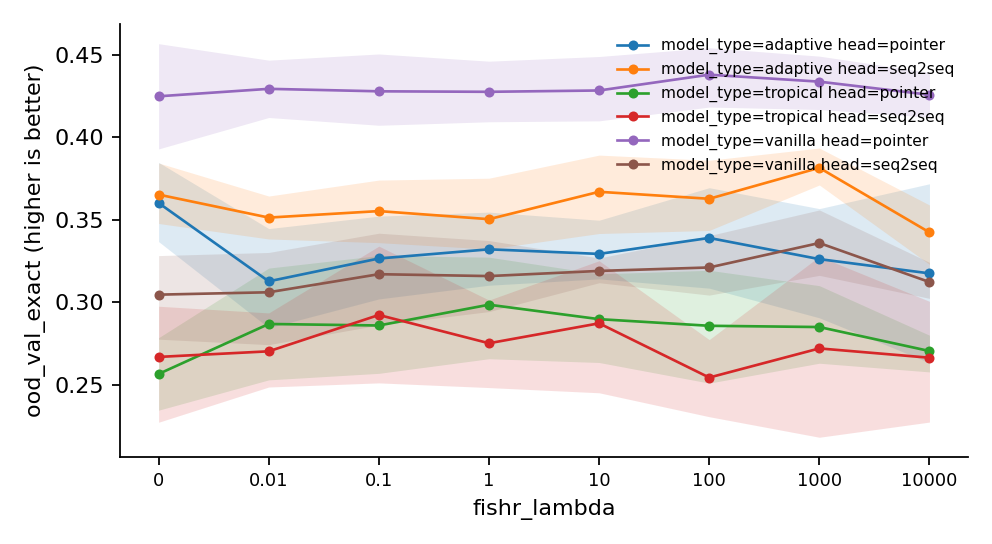
\includegraphics[width=\textwidth]{metric_ood_val_exact.png}
\caption{\texttt{ood\_val\_exact} against \texttt{fishr\_lambda}: the mean over seeds with a 95\% bootstrap CI, one line per combination of the other factors.}
\label{fig:ood_val_exact}
\end{figure}

{\small
\begin{longtable}{lllrlrrr}
\caption{\texttt{ood\_val\_exact} per cell: mean, 95\% bootstrap CI, SD, seeds, diverged runs.}\label{tab:summary-ood_val_exact}\\
\toprule
\texttt{model\_type} & \texttt{head} & \texttt{fishr\_lambda} & mean & 95\% CI & SD & $n$ & div.\\
\midrule
\endhead
adaptive & pointer & 0 & 0.3602 & [0.337, 0.385] & 0.0312 & 5 & 0\\
adaptive & pointer & 0.01 & 0.3127 & [0.285, 0.345] & 0.0387 & 5 & 0\\
adaptive & pointer & 0.1 & 0.3266 & [0.302, 0.352] & 0.0337 & 5 & 0\\
adaptive & pointer & 1 & 0.3321 & [0.31, 0.355] & 0.0298 & 5 & 0\\
adaptive & pointer & 10 & 0.3294 & [0.314, 0.35] & 0.0229 & 5 & 0\\
adaptive & pointer & 100 & 0.339 & [0.309, 0.369] & 0.0381 & 5 & 0\\
adaptive & pointer & 1000 & 0.3262 & [0.291, 0.357] & 0.044 & 5 & 0\\
adaptive & pointer & 1e+04 & 0.3176 & [0.263, 0.372] & 0.0681 & 5 & 0\\
adaptive & seq2seq & 0 & 0.3653 & [0.348, 0.384] & 0.0234 & 5 & 0\\
adaptive & seq2seq & 0.01 & 0.3514 & [0.338, 0.364] & 0.0178 & 5 & 0\\
adaptive & seq2seq & 0.1 & 0.3553 & [0.336, 0.374] & 0.0242 & 5 & 0\\
adaptive & seq2seq & 1 & 0.3504 & [0.332, 0.375] & 0.0278 & 5 & 0\\
adaptive & seq2seq & 10 & 0.367 & [0.342, 0.389] & 0.0324 & 5 & 0\\
adaptive & seq2seq & 100 & 0.3628 & [0.344, 0.386] & 0.0267 & 5 & 0\\
adaptive & seq2seq & 1000 & 0.3816 & [0.371, 0.394] & 0.014 & 5 & 0\\
adaptive & seq2seq & 1e+04 & 0.3424 & [0.323, 0.359] & 0.0235 & 5 & 0\\
tropical & pointer & 0 & 0.2566 & [0.235, 0.279] & 0.0295 & 5 & 0\\
tropical & pointer & 0.01 & 0.2869 & [0.253, 0.321] & 0.0425 & 5 & 0\\
tropical & pointer & 0.1 & 0.286 & [0.257, 0.328] & 0.0459 & 5 & 0\\
tropical & pointer & 1 & 0.2986 & [0.266, 0.327] & 0.0373 & 5 & 0\\
tropical & pointer & 10 & 0.2898 & [0.264, 0.317] & 0.0331 & 5 & 0\\
tropical & pointer & 100 & 0.2858 & [0.251, 0.319] & 0.044 & 5 & 0\\
tropical & pointer & 1000 & 0.285 & [0.263, 0.31] & 0.0298 & 5 & 0\\
tropical & pointer & 1e+04 & 0.2705 & [0.258, 0.28] & 0.0149 & 5 & 0\\
tropical & seq2seq & 0 & 0.2669 & [0.227, 0.298] & 0.0441 & 5 & 0\\
tropical & seq2seq & 0.01 & 0.2703 & [0.249, 0.294] & 0.0298 & 5 & 0\\
tropical & seq2seq & 0.1 & 0.2923 & [0.251, 0.334] & 0.0551 & 5 & 0\\
tropical & seq2seq & 1 & 0.2752 & [0.248, 0.301] & 0.0355 & 5 & 0\\
tropical & seq2seq & 10 & 0.2873 & [0.245, 0.325] & 0.0513 & 5 & 0\\
tropical & seq2seq & 100 & 0.2544 & [0.231, 0.277] & 0.0307 & 5 & 0\\
tropical & seq2seq & 1000 & 0.2721 & [0.218, 0.328] & 0.0731 & 5 & 0\\
tropical & seq2seq & 1e+04 & 0.2664 & [0.227, 0.301] & 0.0499 & 5 & 0\\
vanilla & pointer & 0 & 0.4249 & [0.393, 0.457] & 0.0411 & 5 & 0\\
vanilla & pointer & 0.01 & 0.4294 & [0.412, 0.447] & 0.0229 & 5 & 0\\
vanilla & pointer & 0.1 & 0.4279 & [0.407, 0.451] & 0.0301 & 5 & 0\\
vanilla & pointer & 1 & 0.4276 & [0.409, 0.446] & 0.0237 & 5 & 0\\
vanilla & pointer & 10 & 0.4284 & [0.41, 0.449] & 0.0255 & 5 & 0\\
vanilla & pointer & 100 & 0.438 & [0.418, 0.454] & 0.0235 & 5 & 0\\
vanilla & pointer & 1000 & 0.4338 & [0.417, 0.449] & 0.0207 & 5 & 0\\
vanilla & pointer & 1e+04 & 0.4258 & [0.412, 0.439] & 0.0178 & 5 & 0\\
vanilla & seq2seq & 0 & 0.3047 & [0.278, 0.328] & 0.0326 & 5 & 0\\
vanilla & seq2seq & 0.01 & 0.3061 & [0.274, 0.33] & 0.0363 & 5 & 0\\
vanilla & seq2seq & 0.1 & 0.3171 & [0.286, 0.342] & 0.038 & 5 & 0\\
vanilla & seq2seq & 1 & 0.3159 & [0.294, 0.337] & 0.0281 & 5 & 0\\
vanilla & seq2seq & 10 & 0.319 & [0.312, 0.327] & 0.00961 & 5 & 0\\
vanilla & seq2seq & 100 & 0.3211 & [0.304, 0.34] & 0.0237 & 5 & 0\\
vanilla & seq2seq & 1000 & 0.336 & [0.316, 0.356] & 0.025 & 5 & 0\\
vanilla & seq2seq & 1e+04 & 0.3123 & [0.302, 0.324] & 0.0139 & 5 & 0\\
\bottomrule
\end{longtable}
}

{\small
\begin{longtable}{lllrrrl}
\caption{\texttt{ood\_val\_exact}: each level of \texttt{fishr\_lambda} against its control (0), within each combination of the other factors. parametric: Dunnett vs control.}\label{tab:control-ood_val_exact}\\
\toprule
\texttt{model\_type} & \texttt{head} & \texttt{fishr\_lambda} & difference & 95\% CI & $p$ & \\
\midrule
\endhead
adaptive & pointer & 0.01 & -0.0475 & [-0.118, 0.023] & 0.3024 & \\
adaptive & pointer & 0.1 & -0.03366 & [-0.104, 0.0369] & 0.6462 & \\
adaptive & pointer & 1 & -0.0281 & [-0.0986, 0.0424] & 0.7949 & \\
adaptive & pointer & 10 & -0.03088 & [-0.101, 0.0397] & 0.7226 & \\
adaptive & pointer & 100 & -0.0212 & [-0.0917, 0.0493] & 0.9328 & \\
adaptive & pointer & 1000 & -0.03404 & [-0.105, 0.0365] & 0.6355 & \\
adaptive & pointer & 1e+04 & -0.04268 & [-0.113, 0.0279] & 0.4074 & \\
adaptive & seq2seq & 0.01 & -0.01394 & [-0.0565, 0.0286] & 0.9019 & \\
adaptive & seq2seq & 0.1 & -0.01 & [-0.0525, 0.0325] & 0.9798 & \\
adaptive & seq2seq & 1 & -0.0149 & [-0.0574, 0.0276] & 0.8716 & \\
adaptive & seq2seq & 10 & 0.0017 & [-0.0408, 0.0442] & 1.0000 & \\
adaptive & seq2seq & 100 & -0.00254 & [-0.0451, 0.04] & 1.0000 & \\
adaptive & seq2seq & 1000 & 0.01624 & [-0.0263, 0.0588] & 0.8227 & \\
adaptive & seq2seq & 1e+04 & -0.0229 & [-0.0654, 0.0196] & 0.5266 & \\
tropical & pointer & 0.01 & 0.0303 & [-0.0324, 0.093] & 0.6344 & \\
tropical & pointer & 0.1 & 0.02938 & [-0.0333, 0.0921] & 0.6633 & \\
tropical & pointer & 1 & 0.04198 & [-0.0207, 0.105] & 0.3080 & \\
tropical & pointer & 10 & 0.03322 & [-0.0295, 0.0959] & 0.5437 & \\
tropical & pointer & 100 & 0.0292 & [-0.0335, 0.0919] & 0.6687 & \\
tropical & pointer & 1000 & 0.02844 & [-0.0343, 0.0912] & 0.6924 & \\
tropical & pointer & 1e+04 & 0.0139 & [-0.0488, 0.0766] & 0.9854 & \\
tropical & seq2seq & 0.01 & 0.0034 & [-0.0807, 0.0875] & 1.0000 & \\
tropical & seq2seq & 0.1 & 0.02544 & [-0.0586, 0.11] & 0.9308 & \\
tropical & seq2seq & 1 & 0.0083 & [-0.0758, 0.0924] & 0.9999 & \\
tropical & seq2seq & 10 & 0.02038 & [-0.0637, 0.104] & 0.9764 & \\
tropical & seq2seq & 100 & -0.0125 & [-0.0966, 0.0716] & 0.9986 & \\
tropical & seq2seq & 1000 & 0.00516 & [-0.0789, 0.0892] & 1.0000 & \\
tropical & seq2seq & 1e+04 & $-4.800\times10^{-4}$ & [-0.0846, 0.0836] & 1.0000 & \\
vanilla & pointer & 0.01 & 0.00452 & [-0.0418, 0.0509] & 0.9999 & \\
vanilla & pointer & 0.1 & 0.00302 & [-0.0433, 0.0494] & 1.0000 & \\
vanilla & pointer & 1 & 0.00272 & [-0.0436, 0.0491] & 1.0000 & \\
vanilla & pointer & 10 & 0.00352 & [-0.0428, 0.0499] & 1.0000 & \\
vanilla & pointer & 100 & 0.0131 & [-0.0332, 0.0594] & 0.9494 & \\
vanilla & pointer & 1000 & 0.00888 & [-0.0375, 0.0552] & 0.9935 & \\
vanilla & pointer & 1e+04 & $9.200\times10^{-4}$ & [-0.0454, 0.0473] & 1.0000 & \\
vanilla & seq2seq & 0.01 & 0.00144 & [-0.0468, 0.0497] & 1.0000 & \\
vanilla & seq2seq & 0.1 & 0.0124 & [-0.0358, 0.0606] & 0.9681 & \\
vanilla & seq2seq & 1 & 0.01126 & [-0.037, 0.0595] & 0.9806 & \\
vanilla & seq2seq & 10 & 0.01438 & [-0.0338, 0.0626] & 0.9351 & \\
vanilla & seq2seq & 100 & 0.01648 & [-0.0317, 0.0647] & 0.8837 & \\
vanilla & seq2seq & 1000 & 0.0313 & [-0.0169, 0.0795] & 0.3372 & \\
vanilla & seq2seq & 1e+04 & 0.00764 & [-0.0406, 0.0559] & 0.9979 & \\
\bottomrule
\end{longtable}
}

{\small
\begin{longtable}{llrrrrr}
\caption{\texttt{ood\_val\_exact} against log10 \texttt{fishr\_lambda}: parametric: OLS slope t-test, seed-bootstrap CI, with the Jonckheere--Terpstra ordered-trend $\tau$ and $p$.}\label{tab:trend-ood_val_exact}\\
\toprule
\texttt{model\_type} & \texttt{head} & estimate & 95\% CI & $p$ & JT $\tau$ & JT $p$\\
\midrule
\endhead
adaptive & pointer & $7.357\times10^{-4}$ & [-0.00669, 0.00843] & 0.8254 & 0.103 & 0.4461\\
adaptive & seq2seq & 0.001356 & [$-7.58\times10^{-4}$, 0.00347] & 0.5343 & 0.107 & 0.4159\\
tropical & pointer & -0.002281 & [-0.00805, 0.00366] & 0.4387 & -0.08 & 0.5449\\
tropical & seq2seq & -0.002607 & [-0.00599, 0.00119] & 0.5085 & -0.0705 & 0.6107\\
vanilla & pointer & $4.036\times10^{-4}$ & [-0.00165, 0.0031] & 0.8312 & 0.0362 & 0.7808\\
vanilla & seq2seq & 0.002201 & [-0.00291, 0.00989] & 0.3207 & 0.0267 & 0.8556\\
\bottomrule
\end{longtable}
}

{\small
\begin{longtable}{lrrrl}
\caption{\texttt{ood\_val\_exact}: paired contrasts by seed, Holm-corrected across the cells. parametric: paired t-test by seed, Holm.}\label{tab:paired-ood_val_exact}\\
\toprule
contrast (within) & difference & 95\% CI & $p$ & \\
\midrule
\endhead
\stackcell{model\_type: tropical - vanilla\\\footnotesize head=pointer fishr\_lambda=0 } & -0.1683 & [-0.223, -0.114] & 0.0144 & *\\
\stackcell{model\_type: tropical - vanilla\\\footnotesize head=pointer fishr\_lambda=0.01 } & -0.1426 & [-0.189, -0.0962] & 0.0144 & *\\
\stackcell{model\_type: tropical - vanilla\\\footnotesize head=pointer fishr\_lambda=0.1 } & -0.142 & [-0.221, -0.063] & 0.0677 & \\
\stackcell{model\_type: tropical - vanilla\\\footnotesize head=pointer fishr\_lambda=1 } & -0.1291 & [-0.196, -0.0619] & 0.0607 & \\
\stackcell{model\_type: tropical - vanilla\\\footnotesize head=pointer fishr\_lambda=10 } & -0.1386 & [-0.173, -0.104] & 0.0054 & *\\
\stackcell{model\_type: tropical - vanilla\\\footnotesize head=pointer fishr\_lambda=100 } & -0.1522 & [-0.23, -0.0747] & 0.0607 & \\
\stackcell{model\_type: tropical - vanilla\\\footnotesize head=pointer fishr\_lambda=1000 } & -0.1488 & [-0.203, -0.0941] & 0.0198 & *\\
\stackcell{model\_type: tropical - vanilla\\\footnotesize head=pointer fishr\_lambda=1e+04 } & -0.1554 & [-0.189, -0.122] & 0.0032 & *\\
\stackcell{model\_type: tropical - vanilla\\\footnotesize head=seq2seq fishr\_lambda=0 } & -0.03776 & [-0.109, 0.0335] & 1.0000 & \\
\stackcell{model\_type: tropical - vanilla\\\footnotesize head=seq2seq fishr\_lambda=0.01 } & -0.0358 & [-0.104, 0.0327] & 1.0000 & \\
\stackcell{model\_type: tropical - vanilla\\\footnotesize head=seq2seq fishr\_lambda=0.1 } & -0.02472 & [-0.137, 0.0873] & 1.0000 & \\
\stackcell{model\_type: tropical - vanilla\\\footnotesize head=seq2seq fishr\_lambda=1 } & -0.04072 & [-0.117, 0.0358] & 1.0000 & \\
\stackcell{model\_type: tropical - vanilla\\\footnotesize head=seq2seq fishr\_lambda=10 } & -0.03176 & [-0.0944, 0.0308] & 1.0000 & \\
\stackcell{model\_type: tropical - vanilla\\\footnotesize head=seq2seq fishr\_lambda=100 } & -0.06674 & [-0.129, -0.00398] & 0.3349 & \\
\stackcell{model\_type: tropical - vanilla\\\footnotesize head=seq2seq fishr\_lambda=1000 } & -0.0639 & [-0.143, 0.0155] & 0.6251 & \\
\stackcell{model\_type: tropical - vanilla\\\footnotesize head=seq2seq fishr\_lambda=1e+04 } & -0.04588 & [-0.123, 0.0317] & 1.0000 & \\
\stackcell{model\_type: adaptive - vanilla\\\footnotesize head=pointer fishr\_lambda=0 } & -0.06468 & [-0.124, -0.00489] & 0.2582 & \\
\stackcell{model\_type: adaptive - vanilla\\\footnotesize head=pointer fishr\_lambda=0.01 } & -0.1167 & [-0.179, -0.0546] & 0.0964 & \\
\stackcell{model\_type: adaptive - vanilla\\\footnotesize head=pointer fishr\_lambda=0.1 } & -0.1014 & [-0.169, -0.0335] & 0.1719 & \\
\stackcell{model\_type: adaptive - vanilla\\\footnotesize head=pointer fishr\_lambda=1 } & -0.0955 & [-0.156, -0.0354] & 0.1623 & \\
\stackcell{model\_type: adaptive - vanilla\\\footnotesize head=pointer fishr\_lambda=10 } & -0.09908 & [-0.139, -0.0591] & 0.0373 & *\\
\stackcell{model\_type: adaptive - vanilla\\\footnotesize head=pointer fishr\_lambda=100 } & -0.09898 & [-0.167, -0.0305] & 0.1751 & \\
\stackcell{model\_type: adaptive - vanilla\\\footnotesize head=pointer fishr\_lambda=1000 } & -0.1076 & [-0.183, -0.0324] & 0.1751 & \\
\stackcell{model\_type: adaptive - vanilla\\\footnotesize head=pointer fishr\_lambda=1e+04 } & -0.1083 & [-0.191, -0.0256] & 0.1987 & \\
\stackcell{model\_type: adaptive - vanilla\\\footnotesize head=seq2seq fishr\_lambda=0 } & 0.06066 & [0.0221, 0.0992] & 0.1623 & \\
\stackcell{model\_type: adaptive - vanilla\\\footnotesize head=seq2seq fishr\_lambda=0.01 } & 0.04528 & [-0.00867, 0.0992] & 0.3209 & \\
\stackcell{model\_type: adaptive - vanilla\\\footnotesize head=seq2seq fishr\_lambda=0.1 } & 0.03826 & [-0.0301, 0.107] & 0.3209 & \\
\stackcell{model\_type: adaptive - vanilla\\\footnotesize head=seq2seq fishr\_lambda=1 } & 0.0345 & [0.00212, 0.0669] & 0.2582 & \\
\stackcell{model\_type: adaptive - vanilla\\\footnotesize head=seq2seq fishr\_lambda=10 } & 0.04798 & [0.00997, 0.086] & 0.1987 & \\
\stackcell{model\_type: adaptive - vanilla\\\footnotesize head=seq2seq fishr\_lambda=100 } & 0.04164 & [-0.013, 0.0963] & 0.3209 & \\
\stackcell{model\_type: adaptive - vanilla\\\footnotesize head=seq2seq fishr\_lambda=1000 } & 0.0456 & [0.00451, 0.0867] & 0.2582 & \\
\stackcell{model\_type: adaptive - vanilla\\\footnotesize head=seq2seq fishr\_lambda=1e+04 } & 0.03012 & [-0.0117, 0.072] & 0.3209 & \\
\stackcell{head: pointer - seq2seq\\\footnotesize model\_type=adaptive fishr\_lambda=0 } & -0.00508 & [-0.0394, 0.0293] & 1.0000 & \\
\stackcell{head: pointer - seq2seq\\\footnotesize model\_type=adaptive fishr\_lambda=0.01 } & -0.03864 & [-0.0781, $8.02\times10^{-4}$] & 0.7948 & \\
\stackcell{head: pointer - seq2seq\\\footnotesize model\_type=adaptive fishr\_lambda=0.1 } & -0.02874 & [-0.0459, -0.0116] & 0.1537 & \\
\stackcell{head: pointer - seq2seq\\\footnotesize model\_type=adaptive fishr\_lambda=1 } & -0.01828 & [-0.0614, 0.0248] & 1.0000 & \\
\stackcell{head: pointer - seq2seq\\\footnotesize model\_type=adaptive fishr\_lambda=10 } & -0.03766 & [-0.0784, 0.00308] & 0.8710 & \\
\stackcell{head: pointer - seq2seq\\\footnotesize model\_type=adaptive fishr\_lambda=100 } & -0.02374 & [-0.0803, 0.0328] & 1.0000 & \\
\stackcell{head: pointer - seq2seq\\\footnotesize model\_type=adaptive fishr\_lambda=1000 } & -0.05536 & [-0.116, 0.00558] & 0.8710 & \\
\stackcell{head: pointer - seq2seq\\\footnotesize model\_type=adaptive fishr\_lambda=1e+04 } & -0.02486 & [-0.0886, 0.0388] & 1.0000 & \\
\stackcell{head: pointer - seq2seq\\\footnotesize model\_type=tropical fishr\_lambda=0 } & -0.01032 & [-0.0475, 0.0269] & 1.0000 & \\
\stackcell{head: pointer - seq2seq\\\footnotesize model\_type=tropical fishr\_lambda=0.01 } & 0.01658 & [-0.0708, 0.104] & 1.0000 & \\
\stackcell{head: pointer - seq2seq\\\footnotesize model\_type=tropical fishr\_lambda=0.1 } & -0.00638 & [-0.0637, 0.051] & 1.0000 & \\
\stackcell{head: pointer - seq2seq\\\footnotesize model\_type=tropical fishr\_lambda=1 } & 0.02336 & [-0.0213, 0.0681] & 1.0000 & \\
\stackcell{head: pointer - seq2seq\\\footnotesize model\_type=tropical fishr\_lambda=10 } & 0.00252 & [-0.0815, 0.0866] & 1.0000 & \\
\stackcell{head: pointer - seq2seq\\\footnotesize model\_type=tropical fishr\_lambda=100 } & 0.03138 & [-0.0259, 0.0887] & 1.0000 & \\
\stackcell{head: pointer - seq2seq\\\footnotesize model\_type=tropical fishr\_lambda=1000 } & 0.01296 & [-0.0604, 0.0863] & 1.0000 & \\
\stackcell{head: pointer - seq2seq\\\footnotesize model\_type=tropical fishr\_lambda=1e+04 } & 0.00406 & [-0.046, 0.0541] & 1.0000 & \\
\stackcell{head: pointer - seq2seq\\\footnotesize model\_type=vanilla fishr\_lambda=0 } & 0.1203 & [0.0762, 0.164] & 0.0324 & *\\
\stackcell{head: pointer - seq2seq\\\footnotesize model\_type=vanilla fishr\_lambda=0.01 } & 0.1233 & [0.0972, 0.149] & 0.0041 & *\\
\stackcell{head: pointer - seq2seq\\\footnotesize model\_type=vanilla fishr\_lambda=0.1 } & 0.1109 & [0.0884, 0.133] & 0.0036 & *\\
\stackcell{head: pointer - seq2seq\\\footnotesize model\_type=vanilla fishr\_lambda=1 } & 0.1117 & [0.102, 0.121] & 0.0001 & *\\
\stackcell{head: pointer - seq2seq\\\footnotesize model\_type=vanilla fishr\_lambda=10 } & 0.1094 & [0.0692, 0.15] & 0.0324 & *\\
\stackcell{head: pointer - seq2seq\\\footnotesize model\_type=vanilla fishr\_lambda=100 } & 0.1169 & [0.074, 0.16] & 0.0324 & *\\
\stackcell{head: pointer - seq2seq\\\footnotesize model\_type=vanilla fishr\_lambda=1000 } & 0.09784 & [0.0488, 0.147] & 0.0883 & \\
\stackcell{head: pointer - seq2seq\\\footnotesize model\_type=vanilla fishr\_lambda=1e+04 } & 0.1135 & [0.0975, 0.13] & 0.0009 & *\\
\bottomrule
\end{longtable}
}

\subsection{\texttt{ood\_noise\_f1}}
\begin{figure}[tbp]
\centering
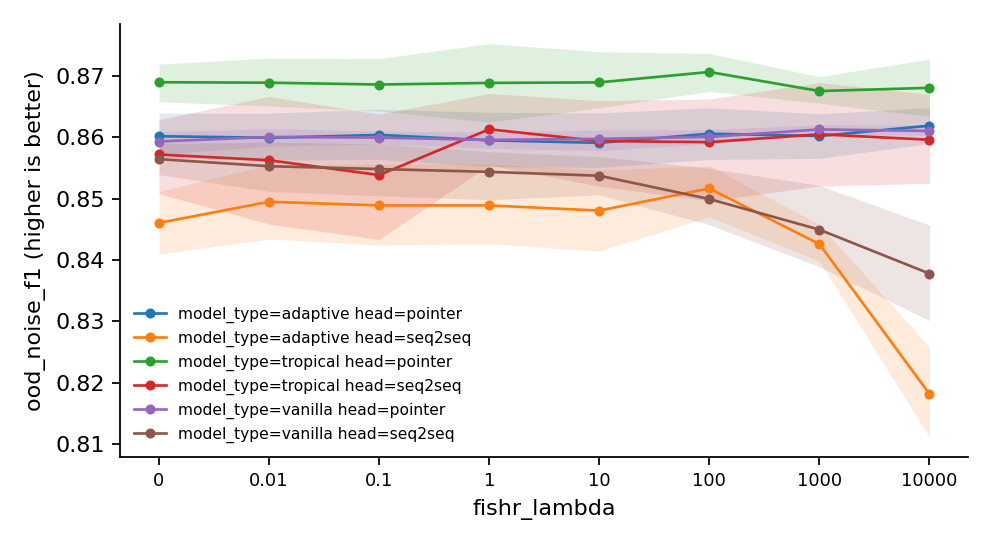
\includegraphics[width=\textwidth]{metric_ood_noise_f1.png}
\caption{\texttt{ood\_noise\_f1} against \texttt{fishr\_lambda}: the mean over seeds with a 95\% bootstrap CI, one line per combination of the other factors.}
\label{fig:ood_noise_f1}
\end{figure}

{\small
\begin{longtable}{lllrlrrr}
\caption{\texttt{ood\_noise\_f1} per cell: mean, 95\% bootstrap CI, SD, seeds, diverged runs.}\label{tab:summary-ood_noise_f1}\\
\toprule
\texttt{model\_type} & \texttt{head} & \texttt{fishr\_lambda} & mean & 95\% CI & SD & $n$ & div.\\
\midrule
\endhead
adaptive & pointer & 0 & 0.8602 & [0.857, 0.864] & 0.0049 & 5 & 0\\
adaptive & pointer & 0.01 & 0.8599 & [0.856, 0.864] & 0.00487 & 5 & 0\\
adaptive & pointer & 0.1 & 0.8604 & [0.856, 0.865] & 0.00536 & 5 & 0\\
adaptive & pointer & 1 & 0.8595 & [0.855, 0.864] & 0.00575 & 5 & 0\\
adaptive & pointer & 10 & 0.8591 & [0.855, 0.864] & 0.00562 & 5 & 0\\
adaptive & pointer & 100 & 0.8606 & [0.856, 0.865] & 0.00542 & 5 & 0\\
adaptive & pointer & 1000 & 0.8602 & [0.857, 0.864] & 0.00458 & 5 & 0\\
adaptive & pointer & 1e+04 & 0.8619 & [0.859, 0.865] & 0.00392 & 5 & 0\\
adaptive & seq2seq & 0 & 0.8461 & [0.841, 0.851] & 0.00663 & 5 & 0\\
adaptive & seq2seq & 0.01 & 0.8495 & [0.843, 0.856] & 0.00779 & 5 & 0\\
adaptive & seq2seq & 0.1 & 0.8489 & [0.842, 0.856] & 0.0086 & 5 & 0\\
adaptive & seq2seq & 1 & 0.8489 & [0.843, 0.856] & 0.0086 & 5 & 0\\
adaptive & seq2seq & 10 & 0.8481 & [0.841, 0.855] & 0.00834 & 5 & 0\\
adaptive & seq2seq & 100 & 0.8517 & [0.847, 0.855] & 0.00545 & 5 & 0\\
adaptive & seq2seq & 1000 & 0.8426 & [0.84, 0.846] & 0.00384 & 5 & 0\\
adaptive & seq2seq & 1e+04 & 0.8181 & [0.811, 0.826] & 0.00954 & 5 & 0\\
tropical & pointer & 0 & 0.869 & [0.866, 0.872] & 0.00394 & 5 & 0\\
tropical & pointer & 0.01 & 0.8689 & [0.865, 0.873] & 0.00524 & 5 & 0\\
tropical & pointer & 0.1 & 0.8686 & [0.864, 0.873] & 0.00545 & 5 & 0\\
tropical & pointer & 1 & 0.8689 & [0.863, 0.875] & 0.00839 & 5 & 0\\
tropical & pointer & 10 & 0.869 & [0.865, 0.874] & 0.00609 & 5 & 0\\
tropical & pointer & 100 & 0.8707 & [0.868, 0.874] & 0.00401 & 5 & 0\\
tropical & pointer & 1000 & 0.8676 & [0.866, 0.87] & 0.00275 & 5 & 0\\
tropical & pointer & 1e+04 & 0.8681 & [0.863, 0.873] & 0.00593 & 5 & 0\\
tropical & seq2seq & 0 & 0.8572 & [0.851, 0.863] & 0.00791 & 5 & 0\\
tropical & seq2seq & 0.01 & 0.8563 & [0.846, 0.867] & 0.0135 & 5 & 0\\
tropical & seq2seq & 0.1 & 0.8539 & [0.843, 0.864] & 0.0134 & 5 & 0\\
tropical & seq2seq & 1 & 0.8613 & [0.855, 0.867] & 0.00774 & 5 & 0\\
tropical & seq2seq & 10 & 0.8594 & [0.852, 0.866] & 0.00916 & 5 & 0\\
tropical & seq2seq & 100 & 0.8592 & [0.85, 0.866] & 0.0109 & 5 & 0\\
tropical & seq2seq & 1000 & 0.8605 & [0.852, 0.869] & 0.011 & 5 & 0\\
tropical & seq2seq & 1e+04 & 0.8596 & [0.853, 0.867] & 0.00946 & 5 & 0\\
vanilla & pointer & 0 & 0.8593 & [0.857, 0.861] & 0.00247 & 5 & 0\\
vanilla & pointer & 0.01 & 0.8601 & [0.859, 0.861] & 0.00177 & 5 & 0\\
vanilla & pointer & 0.1 & 0.86 & [0.859, 0.861] & 0.00138 & 5 & 0\\
vanilla & pointer & 1 & 0.8596 & [0.858, 0.861] & 0.00169 & 5 & 0\\
vanilla & pointer & 10 & 0.8598 & [0.858, 0.861] & 0.00207 & 5 & 0\\
vanilla & pointer & 100 & 0.8601 & [0.859, 0.861] & 0.0015 & 5 & 0\\
vanilla & pointer & 1000 & 0.8613 & [0.861, 0.862] & 0.00103 & 5 & 0\\
vanilla & pointer & 1e+04 & 0.8611 & [0.86, 0.862] & 0.00109 & 5 & 0\\
vanilla & seq2seq & 0 & 0.8565 & [0.854, 0.859] & 0.00345 & 5 & 0\\
vanilla & seq2seq & 0.01 & 0.8553 & [0.851, 0.859] & 0.00523 & 5 & 0\\
vanilla & seq2seq & 0.1 & 0.8548 & [0.85, 0.859] & 0.00541 & 5 & 0\\
vanilla & seq2seq & 1 & 0.8544 & [0.85, 0.858] & 0.00496 & 5 & 0\\
vanilla & seq2seq & 10 & 0.8538 & [0.851, 0.857] & 0.00397 & 5 & 0\\
vanilla & seq2seq & 100 & 0.85 & [0.846, 0.855] & 0.00606 & 5 & 0\\
vanilla & seq2seq & 1000 & 0.845 & [0.839, 0.852] & 0.00853 & 5 & 0\\
vanilla & seq2seq & 1e+04 & 0.8378 & [0.83, 0.846] & 0.01 & 5 & 0\\
\bottomrule
\end{longtable}
}

{\small
\begin{longtable}{lllrrrl}
\caption{\texttt{ood\_noise\_f1}: each level of \texttt{fishr\_lambda} against its control (0), within each combination of the other factors. parametric: Dunnett vs control.}\label{tab:control-ood_noise_f1}\\
\toprule
\texttt{model\_type} & \texttt{head} & \texttt{fishr\_lambda} & difference & 95\% CI & $p$ & \\
\midrule
\endhead
adaptive & pointer & 0.01 & $-2.568\times10^{-4}$ & [-0.00914, 0.00862] & 1.0000 & \\
adaptive & pointer & 0.1 & $2.143\times10^{-4}$ & [-0.00867, 0.0091] & 1.0000 & \\
adaptive & pointer & 1 & $-6.699\times10^{-4}$ & [-0.00955, 0.00821] & 1.0000 & \\
adaptive & pointer & 10 & -0.001082 & [-0.00996, 0.0078] & 0.9996 & \\
adaptive & pointer & 100 & $4.157\times10^{-4}$ & [-0.00847, 0.0093] & 1.0000 & \\
adaptive & pointer & 1000 & $2.933\times10^{-5}$ & [-0.00885, 0.00891] & 1.0000 & \\
adaptive & pointer & 1e+04 & 0.001723 & [-0.00716, 0.0106] & 0.9931 & \\
adaptive & seq2seq & 0.01 & 0.003448 & [-0.00976, 0.0167] & 0.9656 & \\
adaptive & seq2seq & 0.1 & 0.002857 & [-0.0104, 0.0161] & 0.9872 & \\
adaptive & seq2seq & 1 & 0.002852 & [-0.0104, 0.0161] & 0.9873 & \\
adaptive & seq2seq & 10 & 0.002012 & [-0.0112, 0.0152] & 0.9984 & \\
adaptive & seq2seq & 100 & 0.005621 & [-0.00759, 0.0188] & 0.7456 & \\
adaptive & seq2seq & 1000 & -0.003458 & [-0.0167, 0.00975] & 0.9651 & \\
adaptive & seq2seq & 1e+04 & -0.02792 & [-0.0411, -0.0147] & $<10^{-4}$ & *\\
tropical & pointer & 0.01 & $-7.411\times10^{-5}$ & [-0.00962, 0.00947] & 1.0000 & \\
tropical & pointer & 0.1 & $-3.733\times10^{-4}$ & [-0.00992, 0.00917] & 1.0000 & \\
tropical & pointer & 1 & $-1.089\times10^{-4}$ & [-0.00965, 0.00944] & 1.0000 & \\
tropical & pointer & 10 & $-2.563\times10^{-5}$ & [-0.00957, 0.00952] & 1.0000 & \\
tropical & pointer & 100 & 0.001674 & [-0.00787, 0.0112] & 0.9962 & \\
tropical & pointer & 1000 & -0.001438 & [-0.011, 0.00811] & 0.9985 & \\
tropical & pointer & 1e+04 & $-9.146\times10^{-4}$ & [-0.0105, 0.00863] & 0.9999 & \\
tropical & seq2seq & 0.01 & $-9.374\times10^{-4}$ & [-0.0195, 0.0176] & 1.0000 & \\
tropical & seq2seq & 0.1 & -0.00335 & [-0.0219, 0.0152] & 0.9954 & \\
tropical & seq2seq & 1 & 0.004111 & [-0.0144, 0.0226] & 0.9852 & \\
tropical & seq2seq & 10 & 0.002193 & [-0.0163, 0.0207] & 0.9997 & \\
tropical & seq2seq & 100 & 0.002015 & [-0.0165, 0.0205] & 0.9998 & \\
tropical & seq2seq & 1000 & 0.003296 & [-0.0152, 0.0218] & 0.9958 & \\
tropical & seq2seq & 1e+04 & 0.002406 & [-0.0161, 0.0209] & 0.9994 & \\
vanilla & pointer & 0.01 & $7.460\times10^{-4}$ & [-0.0022, 0.00369] & 0.9706 & \\
vanilla & pointer & 0.1 & $6.349\times10^{-4}$ & [-0.00231, 0.00358] & 0.9875 & \\
vanilla & pointer & 1 & $2.582\times10^{-4}$ & [-0.00269, 0.00321] & 1.0000 & \\
vanilla & pointer & 10 & $4.334\times10^{-4}$ & [-0.00252, 0.00338] & 0.9987 & \\
vanilla & pointer & 100 & $7.489\times10^{-4}$ & [-0.0022, 0.0037] & 0.9700 & \\
vanilla & pointer & 1000 & 0.00197 & [$-9.79\times10^{-4}$, 0.00492] & 0.3098 & \\
vanilla & pointer & 1e+04 & 0.00172 & [-0.00123, 0.00467] & 0.4448 & \\
vanilla & seq2seq & 0.01 & -0.001154 & [-0.0122, 0.00988] & 0.9999 & \\
vanilla & seq2seq & 0.1 & -0.001621 & [-0.0127, 0.00941] & 0.9987 & \\
vanilla & seq2seq & 1 & -0.002078 & [-0.0131, 0.00896] & 0.9942 & \\
vanilla & seq2seq & 10 & -0.002708 & [-0.0137, 0.00833] & 0.9748 & \\
vanilla & seq2seq & 100 & -0.006512 & [-0.0175, 0.00452] & 0.4329 & \\
vanilla & seq2seq & 1000 & -0.0115 & [-0.0225, $-4.68\times10^{-4}$] & 0.0381 & *\\
vanilla & seq2seq & 1e+04 & -0.01868 & [-0.0297, -0.00764] & 0.0003 & *\\
\bottomrule
\end{longtable}
}

{\small
\begin{longtable}{llrrrrr}
\caption{\texttt{ood\_noise\_f1} against log10 \texttt{fishr\_lambda}: parametric: OLS slope t-test, seed-bootstrap CI, with the Jonckheere--Terpstra ordered-trend $\tau$ and $p$.}\label{tab:trend-ood_noise_f1}\\
\toprule
\texttt{model\_type} & \texttt{head} & estimate & 95\% CI & $p$ & JT $\tau$ & JT $p$\\
\midrule
\endhead
adaptive & pointer & $2.377\times10^{-4}$ & [$4.38\times10^{-5}$, $3.89\times10^{-4}$] & 0.5585 & 0.0857 & 0.5355\\
adaptive & seq2seq & -0.003713 & [-0.00494, -0.00282] & 0.0003 & -0.406 & 0.0028\\
tropical & pointer & $-1.024\times10^{-4}$ & [-0.00118, $8.13\times10^{-4}$] & 0.8199 & -0.0324 & 0.8260\\
tropical & seq2seq & $7.582\times10^{-4}$ & [$-5.37\times10^{-5}$, 0.00158] & 0.3879 & 0.0895 & 0.5149\\
vanilla & pointer & $2.172\times10^{-4}$ & [$1.01\times10^{-4}$, $3.79\times10^{-4}$] & 0.0930 & 0.219 & 0.1008\\
vanilla & seq2seq & -0.002742 & [-0.00384, -0.00206] & $<10^{-4}$ & -0.505 & 0.0004\\
\bottomrule
\end{longtable}
}

{\small
\begin{longtable}{lrrrl}
\caption{\texttt{ood\_noise\_f1}: paired contrasts by seed, Holm-corrected across the cells. parametric: paired t-test by seed, Holm.}\label{tab:paired-ood_noise_f1}\\
\toprule
contrast (within) & difference & 95\% CI & $p$ & \\
\midrule
\endhead
\stackcell{model\_type: tropical - vanilla\\\footnotesize head=pointer fishr\_lambda=0 } & 0.00967 & [0.00215, 0.0172] & 0.3039 & \\
\stackcell{model\_type: tropical - vanilla\\\footnotesize head=pointer fishr\_lambda=0.01 } & 0.00885 & [$5.81\times10^{-4}$, 0.0171] & 0.4518 & \\
\stackcell{model\_type: tropical - vanilla\\\footnotesize head=pointer fishr\_lambda=0.1 } & 0.008662 & [$3.25\times10^{-4}$, 0.017] & 0.4518 & \\
\stackcell{model\_type: tropical - vanilla\\\footnotesize head=pointer fishr\_lambda=1 } & 0.009303 & [-0.00275, 0.0214] & 0.7685 & \\
\stackcell{model\_type: tropical - vanilla\\\footnotesize head=pointer fishr\_lambda=10 } & 0.009211 & [0.00162, 0.0168] & 0.3372 & \\
\stackcell{model\_type: tropical - vanilla\\\footnotesize head=pointer fishr\_lambda=100 } & 0.0106 & [0.00397, 0.0172] & 0.1585 & \\
\stackcell{model\_type: tropical - vanilla\\\footnotesize head=pointer fishr\_lambda=1000 } & 0.006263 & [0.0026, 0.00993] & 0.1352 & \\
\stackcell{model\_type: tropical - vanilla\\\footnotesize head=pointer fishr\_lambda=1e+04 } & 0.007036 & [$1.61\times10^{-4}$, 0.0139] & 0.4518 & \\
\stackcell{model\_type: tropical - vanilla\\\footnotesize head=seq2seq fishr\_lambda=0 } & $7.552\times10^{-4}$ & [-0.0125, 0.014] & 1.0000 & \\
\stackcell{model\_type: tropical - vanilla\\\footnotesize head=seq2seq fishr\_lambda=0.01 } & $9.717\times10^{-4}$ & [-0.0154, 0.0174] & 1.0000 & \\
\stackcell{model\_type: tropical - vanilla\\\footnotesize head=seq2seq fishr\_lambda=0.1 } & $-9.738\times10^{-4}$ & [-0.0187, 0.0167] & 1.0000 & \\
\stackcell{model\_type: tropical - vanilla\\\footnotesize head=seq2seq fishr\_lambda=1 } & 0.006944 & [-0.00285, 0.0167] & 0.7685 & \\
\stackcell{model\_type: tropical - vanilla\\\footnotesize head=seq2seq fishr\_lambda=10 } & 0.005656 & [-0.00233, 0.0136] & 0.7685 & \\
\stackcell{model\_type: tropical - vanilla\\\footnotesize head=seq2seq fishr\_lambda=100 } & 0.009282 & [-0.00384, 0.0224] & 0.7685 & \\
\stackcell{model\_type: tropical - vanilla\\\footnotesize head=seq2seq fishr\_lambda=1000 } & 0.01556 & [-0.00437, 0.0355] & 0.7685 & \\
\stackcell{model\_type: tropical - vanilla\\\footnotesize head=seq2seq fishr\_lambda=1e+04 } & 0.02184 & [0.0124, 0.0312] & 0.0476 & *\\
\stackcell{model\_type: adaptive - vanilla\\\footnotesize head=pointer fishr\_lambda=0 } & $8.617\times10^{-4}$ & [-0.00546, 0.00719] & 1.0000 & \\
\stackcell{model\_type: adaptive - vanilla\\\footnotesize head=pointer fishr\_lambda=0.01 } & $-1.410\times10^{-4}$ & [-0.00606, 0.00578] & 1.0000 & \\
\stackcell{model\_type: adaptive - vanilla\\\footnotesize head=pointer fishr\_lambda=0.1 } & $4.411\times10^{-4}$ & [-0.00622, 0.0071] & 1.0000 & \\
\stackcell{model\_type: adaptive - vanilla\\\footnotesize head=pointer fishr\_lambda=1 } & $-6.638\times10^{-5}$ & [-0.00749, 0.00736] & 1.0000 & \\
\stackcell{model\_type: adaptive - vanilla\\\footnotesize head=pointer fishr\_lambda=10 } & $-6.535\times10^{-4}$ & [-0.00757, 0.00626] & 1.0000 & \\
\stackcell{model\_type: adaptive - vanilla\\\footnotesize head=pointer fishr\_lambda=100 } & $5.285\times10^{-4}$ & [-0.0067, 0.00776] & 1.0000 & \\
\stackcell{model\_type: adaptive - vanilla\\\footnotesize head=pointer fishr\_lambda=1000 } & -0.001079 & [-0.00706, 0.0049] & 1.0000 & \\
\stackcell{model\_type: adaptive - vanilla\\\footnotesize head=pointer fishr\_lambda=1e+04 } & $8.648\times10^{-4}$ & [-0.00396, 0.00569] & 1.0000 & \\
\stackcell{model\_type: adaptive - vanilla\\\footnotesize head=seq2seq fishr\_lambda=0 } & -0.01041 & [-0.0213, $5.21\times10^{-4}$] & 0.8600 & \\
\stackcell{model\_type: adaptive - vanilla\\\footnotesize head=seq2seq fishr\_lambda=0.01 } & -0.005805 & [-0.0206, 0.00901] & 1.0000 & \\
\stackcell{model\_type: adaptive - vanilla\\\footnotesize head=seq2seq fishr\_lambda=0.1 } & -0.005928 & [-0.022, 0.0101] & 1.0000 & \\
\stackcell{model\_type: adaptive - vanilla\\\footnotesize head=seq2seq fishr\_lambda=1 } & -0.005476 & [-0.0211, 0.0101] & 1.0000 & \\
\stackcell{model\_type: adaptive - vanilla\\\footnotesize head=seq2seq fishr\_lambda=10 } & -0.005686 & [-0.0161, 0.00469] & 1.0000 & \\
\stackcell{model\_type: adaptive - vanilla\\\footnotesize head=seq2seq fishr\_lambda=100 } & 0.001727 & [-0.0126, 0.016] & 1.0000 & \\
\stackcell{model\_type: adaptive - vanilla\\\footnotesize head=seq2seq fishr\_lambda=1000 } & -0.00236 & [-0.0171, 0.0123] & 1.0000 & \\
\stackcell{model\_type: adaptive - vanilla\\\footnotesize head=seq2seq fishr\_lambda=1e+04 } & -0.01965 & [-0.0212, -0.0181] & $<10^{-4}$ & *\\
\stackcell{head: pointer - seq2seq\\\footnotesize model\_type=adaptive fishr\_lambda=0 } & 0.01414 & [0.00686, 0.0214] & 0.1199 & \\
\stackcell{head: pointer - seq2seq\\\footnotesize model\_type=adaptive fishr\_lambda=0.01 } & 0.01044 & [$-7.00\times10^{-4}$, 0.0216] & 0.8479 & \\
\stackcell{head: pointer - seq2seq\\\footnotesize model\_type=adaptive fishr\_lambda=0.1 } & 0.0115 & [$-8.89\times10^{-4}$, 0.0239] & 0.8479 & \\
\stackcell{head: pointer - seq2seq\\\footnotesize model\_type=adaptive fishr\_lambda=1 } & 0.01062 & [-0.0033, 0.0245] & 1.0000 & \\
\stackcell{head: pointer - seq2seq\\\footnotesize model\_type=adaptive fishr\_lambda=10 } & 0.01105 & [-0.00278, 0.0249] & 1.0000 & \\
\stackcell{head: pointer - seq2seq\\\footnotesize model\_type=adaptive fishr\_lambda=100 } & 0.008936 & [$2.30\times10^{-4}$, 0.0176] & 0.7889 & \\
\stackcell{head: pointer - seq2seq\\\footnotesize model\_type=adaptive fishr\_lambda=1000 } & 0.01763 & [0.0134, 0.0218] & 0.0074 & *\\
\stackcell{head: pointer - seq2seq\\\footnotesize model\_type=adaptive fishr\_lambda=1e+04 } & 0.04378 & [0.0314, 0.0562] & 0.0139 & *\\
\stackcell{head: pointer - seq2seq\\\footnotesize model\_type=tropical fishr\_lambda=0 } & 0.01179 & [0.00387, 0.0197] & 0.2892 & \\
\stackcell{head: pointer - seq2seq\\\footnotesize model\_type=tropical fishr\_lambda=0.01 } & 0.01265 & [-0.0075, 0.0328] & 1.0000 & \\
\stackcell{head: pointer - seq2seq\\\footnotesize model\_type=tropical fishr\_lambda=0.1 } & 0.01477 & [-0.00335, 0.0329] & 1.0000 & \\
\stackcell{head: pointer - seq2seq\\\footnotesize model\_type=tropical fishr\_lambda=1 } & 0.007569 & [-0.00771, 0.0229] & 1.0000 & \\
\stackcell{head: pointer - seq2seq\\\footnotesize model\_type=tropical fishr\_lambda=10 } & 0.00957 & [-0.00714, 0.0263] & 1.0000 & \\
\stackcell{head: pointer - seq2seq\\\footnotesize model\_type=tropical fishr\_lambda=100 } & 0.01145 & [$-4.69\times10^{-4}$, 0.0234] & 0.8479 & \\
\stackcell{head: pointer - seq2seq\\\footnotesize model\_type=tropical fishr\_lambda=1000 } & 0.007055 & [-0.00712, 0.0212] & 1.0000 & \\
\stackcell{head: pointer - seq2seq\\\footnotesize model\_type=tropical fishr\_lambda=1e+04 } & 0.008468 & [-0.00422, 0.0212] & 1.0000 & \\
\stackcell{head: pointer - seq2seq\\\footnotesize model\_type=vanilla fishr\_lambda=0 } & 0.002874 & [-0.00338, 0.00912] & 1.0000 & \\
\stackcell{head: pointer - seq2seq\\\footnotesize model\_type=vanilla fishr\_lambda=0.01 } & 0.004774 & [-0.00267, 0.0122] & 1.0000 & \\
\stackcell{head: pointer - seq2seq\\\footnotesize model\_type=vanilla fishr\_lambda=0.1 } & 0.00513 & [-0.00246, 0.0127] & 1.0000 & \\
\stackcell{head: pointer - seq2seq\\\footnotesize model\_type=vanilla fishr\_lambda=1 } & 0.00521 & [-0.00176, 0.0122] & 1.0000 & \\
\stackcell{head: pointer - seq2seq\\\footnotesize model\_type=vanilla fishr\_lambda=10 } & 0.006015 & [$-1.25\times10^{-4}$, 0.0122] & 0.8479 & \\
\stackcell{head: pointer - seq2seq\\\footnotesize model\_type=vanilla fishr\_lambda=100 } & 0.01013 & [$8.98\times10^{-4}$, 0.0194] & 0.6869 & \\
\stackcell{head: pointer - seq2seq\\\footnotesize model\_type=vanilla fishr\_lambda=1000 } & 0.01635 & [0.0051, 0.0276] & 0.2975 & \\
\stackcell{head: pointer - seq2seq\\\footnotesize model\_type=vanilla fishr\_lambda=1e+04 } & 0.02327 & [0.0121, 0.0345] & 0.0990 & \\
\bottomrule
\end{longtable}
}

\subsection{\texttt{ood\_noise\_exact}}
\begin{figure}[tbp]
\centering
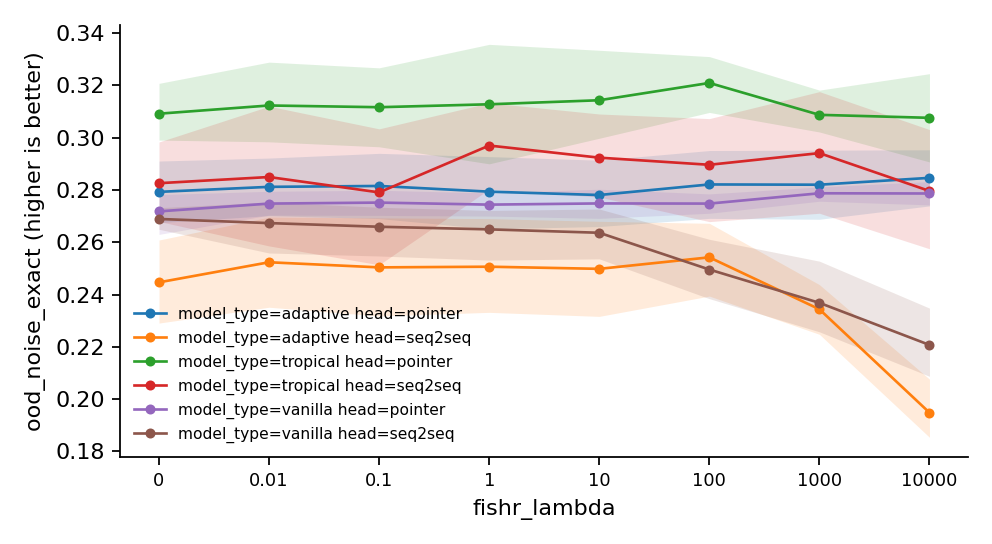
\includegraphics[width=\textwidth]{metric_ood_noise_exact.png}
\caption{\texttt{ood\_noise\_exact} against \texttt{fishr\_lambda}: the mean over seeds with a 95\% bootstrap CI, one line per combination of the other factors.}
\label{fig:ood_noise_exact}
\end{figure}

{\small
\begin{longtable}{lllrlrrr}
\caption{\texttt{ood\_noise\_exact} per cell: mean, 95\% bootstrap CI, SD, seeds, diverged runs.}\label{tab:summary-ood_noise_exact}\\
\toprule
\texttt{model\_type} & \texttt{head} & \texttt{fishr\_lambda} & mean & 95\% CI & SD & $n$ & div.\\
\midrule
\endhead
adaptive & pointer & 0 & 0.2793 & [0.267, 0.291] & 0.0161 & 5 & 0\\
adaptive & pointer & 0.01 & 0.2812 & [0.27, 0.292] & 0.0143 & 5 & 0\\
adaptive & pointer & 0.1 & 0.2815 & [0.269, 0.294] & 0.0165 & 5 & 0\\
adaptive & pointer & 1 & 0.2793 & [0.265, 0.293] & 0.018 & 5 & 0\\
adaptive & pointer & 10 & 0.2781 & [0.266, 0.291] & 0.0162 & 5 & 0\\
adaptive & pointer & 100 & 0.2821 & [0.269, 0.295] & 0.0166 & 5 & 0\\
adaptive & pointer & 1000 & 0.282 & [0.269, 0.295] & 0.0169 & 5 & 0\\
adaptive & pointer & 1e+04 & 0.2846 & [0.274, 0.295] & 0.0142 & 5 & 0\\
adaptive & seq2seq & 0 & 0.2447 & [0.229, 0.261] & 0.0203 & 5 & 0\\
adaptive & seq2seq & 0.01 & 0.2523 & [0.235, 0.27] & 0.0223 & 5 & 0\\
adaptive & seq2seq & 0.1 & 0.2504 & [0.232, 0.269] & 0.0245 & 5 & 0\\
adaptive & seq2seq & 1 & 0.2506 & [0.233, 0.269] & 0.0239 & 5 & 0\\
adaptive & seq2seq & 10 & 0.2498 & [0.232, 0.268] & 0.0234 & 5 & 0\\
adaptive & seq2seq & 100 & 0.2542 & [0.239, 0.267] & 0.0188 & 5 & 0\\
adaptive & seq2seq & 1000 & 0.2344 & [0.225, 0.244] & 0.0123 & 5 & 0\\
adaptive & seq2seq & 1e+04 & 0.1948 & [0.185, 0.208] & 0.0147 & 5 & 0\\
tropical & pointer & 0 & 0.3092 & [0.299, 0.321] & 0.013 & 5 & 0\\
tropical & pointer & 0.01 & 0.3123 & [0.298, 0.329] & 0.0199 & 5 & 0\\
tropical & pointer & 0.1 & 0.3116 & [0.296, 0.327] & 0.0191 & 5 & 0\\
tropical & pointer & 1 & 0.3128 & [0.29, 0.336] & 0.0297 & 5 & 0\\
tropical & pointer & 10 & 0.3143 & [0.3, 0.333] & 0.0225 & 5 & 0\\
tropical & pointer & 100 & 0.3209 & [0.31, 0.331] & 0.0138 & 5 & 0\\
tropical & pointer & 1000 & 0.3087 & [0.302, 0.318] & 0.011 & 5 & 0\\
tropical & pointer & 1e+04 & 0.3076 & [0.291, 0.324] & 0.0216 & 5 & 0\\
tropical & seq2seq & 0 & 0.2826 & [0.268, 0.298] & 0.0206 & 5 & 0\\
tropical & seq2seq & 0.01 & 0.2849 & [0.259, 0.312] & 0.034 & 5 & 0\\
tropical & seq2seq & 0.1 & 0.2791 & [0.251, 0.303] & 0.0331 & 5 & 0\\
tropical & seq2seq & 1 & 0.297 & [0.28, 0.313] & 0.0214 & 5 & 0\\
tropical & seq2seq & 10 & 0.2923 & [0.277, 0.309] & 0.0215 & 5 & 0\\
tropical & seq2seq & 100 & 0.2896 & [0.268, 0.307] & 0.0255 & 5 & 0\\
tropical & seq2seq & 1000 & 0.2941 & [0.271, 0.318] & 0.0306 & 5 & 0\\
tropical & seq2seq & 1e+04 & 0.2796 & [0.258, 0.303] & 0.0293 & 5 & 0\\
vanilla & pointer & 0 & 0.2718 & [0.263, 0.278] & 0.0102 & 5 & 0\\
vanilla & pointer & 0.01 & 0.2748 & [0.27, 0.279] & 0.00601 & 5 & 0\\
vanilla & pointer & 0.1 & 0.2752 & [0.27, 0.28] & 0.00617 & 5 & 0\\
vanilla & pointer & 1 & 0.2744 & [0.27, 0.279] & 0.00566 & 5 & 0\\
vanilla & pointer & 10 & 0.2748 & [0.269, 0.28] & 0.00732 & 5 & 0\\
vanilla & pointer & 100 & 0.2748 & [0.271, 0.278] & 0.00504 & 5 & 0\\
vanilla & pointer & 1000 & 0.2787 & [0.276, 0.281] & 0.00358 & 5 & 0\\
vanilla & pointer & 1e+04 & 0.2786 & [0.274, 0.283] & 0.00582 & 5 & 0\\
vanilla & seq2seq & 0 & 0.2689 & [0.265, 0.273] & 0.00558 & 5 & 0\\
vanilla & seq2seq & 0.01 & 0.2673 & [0.256, 0.275] & 0.0127 & 5 & 0\\
vanilla & seq2seq & 0.1 & 0.2659 & [0.255, 0.273] & 0.0124 & 5 & 0\\
vanilla & seq2seq & 1 & 0.2649 & [0.253, 0.272] & 0.0132 & 5 & 0\\
vanilla & seq2seq & 10 & 0.2636 & [0.254, 0.273] & 0.0123 & 5 & 0\\
vanilla & seq2seq & 100 & 0.2496 & [0.238, 0.261] & 0.015 & 5 & 0\\
vanilla & seq2seq & 1000 & 0.2368 & [0.226, 0.253] & 0.018 & 5 & 0\\
vanilla & seq2seq & 1e+04 & 0.2207 & [0.209, 0.235] & 0.0171 & 5 & 0\\
\bottomrule
\end{longtable}
}

{\small
\begin{longtable}{lllrrrl}
\caption{\texttt{ood\_noise\_exact}: each level of \texttt{fishr\_lambda} against its control (0), within each combination of the other factors. parametric: Dunnett vs control.}\label{tab:control-ood_noise_exact}\\
\toprule
\texttt{model\_type} & \texttt{head} & \texttt{fishr\_lambda} & difference & 95\% CI & $p$ & \\
\midrule
\endhead
adaptive & pointer & 0.01 & 0.00192 & [-0.0263, 0.0301] & 1.0000 & \\
adaptive & pointer & 0.1 & 0.00226 & [-0.026, 0.0305] & 1.0000 & \\
adaptive & pointer & 1 & $8.000\times10^{-5}$ & [-0.0281, 0.0283] & 1.0000 & \\
adaptive & pointer & 10 & -0.0012 & [-0.0294, 0.027] & 1.0000 & \\
adaptive & pointer & 100 & 0.00284 & [-0.0254, 0.0311] & 0.9999 & \\
adaptive & pointer & 1000 & 0.00274 & [-0.0255, 0.031] & 0.9999 & \\
adaptive & pointer & 1e+04 & 0.00536 & [-0.0229, 0.0336] & 0.9939 & \\
adaptive & seq2seq & 0.01 & 0.00768 & [-0.0281, 0.0434] & 0.9876 & \\
adaptive & seq2seq & 0.1 & 0.00572 & [-0.03, 0.0415] & 0.9978 & \\
adaptive & seq2seq & 1 & 0.00598 & [-0.0298, 0.0417] & 0.9971 & \\
adaptive & seq2seq & 10 & 0.00516 & [-0.0306, 0.0409] & 0.9988 & \\
adaptive & seq2seq & 100 & 0.00956 & [-0.0262, 0.0453] & 0.9612 & \\
adaptive & seq2seq & 1000 & -0.0103 & [-0.046, 0.0254] & 0.9446 & \\
adaptive & seq2seq & 1e+04 & -0.04984 & [-0.0856, -0.0141] & 0.0033 & *\\
tropical & pointer & 0.01 & 0.00314 & [-0.0312, 0.0375] & 0.9999 & \\
tropical & pointer & 0.1 & 0.00248 & [-0.0319, 0.0368] & 1.0000 & \\
tropical & pointer & 1 & 0.0036 & [-0.0307, 0.0379] & 0.9999 & \\
tropical & pointer & 10 & 0.00514 & [-0.0292, 0.0395] & 0.9985 & \\
tropical & pointer & 100 & 0.01176 & [-0.0226, 0.0461] & 0.8829 & \\
tropical & pointer & 1000 & $-4.400\times10^{-4}$ & [-0.0348, 0.0339] & 1.0000 & \\
tropical & pointer & 1e+04 & -0.00158 & [-0.0359, 0.0328] & 1.0000 & \\
tropical & seq2seq & 0.01 & 0.00236 & [-0.0457, 0.0504] & 1.0000 & \\
tropical & seq2seq & 0.1 & -0.00352 & [-0.0515, 0.0445] & 1.0000 & \\
tropical & seq2seq & 1 & 0.0144 & [-0.0336, 0.0624] & 0.9335 & \\
tropical & seq2seq & 10 & 0.00976 & [-0.0383, 0.0578] & 0.9909 & \\
tropical & seq2seq & 100 & 0.00704 & [-0.041, 0.0551] & 0.9987 & \\
tropical & seq2seq & 1000 & 0.0115 & [-0.0365, 0.0595] & 0.9778 & \\
tropical & seq2seq & 1e+04 & -0.00298 & [-0.051, 0.045] & 1.0000 & \\
vanilla & pointer & 0.01 & 0.00298 & [-0.00835, 0.0143] & 0.9643 & \\
vanilla & pointer & 0.1 & 0.00336 & [-0.00797, 0.0147] & 0.9369 & \\
vanilla & pointer & 1 & 0.00258 & [-0.00875, 0.0139] & 0.9831 & \\
vanilla & pointer & 10 & 0.00304 & [-0.00829, 0.0144] & 0.9606 & \\
vanilla & pointer & 100 & 0.00298 & [-0.00835, 0.0143] & 0.9643 & \\
vanilla & pointer & 1000 & 0.00692 & [-0.00441, 0.0183] & 0.3980 & \\
vanilla & pointer & 1e+04 & 0.00684 & [-0.00449, 0.0182] & 0.4098 & \\
vanilla & seq2seq & 0.01 & -0.00158 & [-0.0256, 0.0224] & 1.0000 & \\
vanilla & seq2seq & 0.1 & -0.00298 & [-0.027, 0.021] & 0.9996 & \\
vanilla & seq2seq & 1 & -0.00398 & [-0.028, 0.02] & 0.9973 & \\
vanilla & seq2seq & 10 & -0.00528 & [-0.0293, 0.0187] & 0.9860 & \\
vanilla & seq2seq & 100 & -0.01934 & [-0.0434, 0.00468] & 0.1565 & \\
vanilla & seq2seq & 1000 & -0.03208 & [-0.0561, -0.00806] & 0.0050 & *\\
vanilla & seq2seq & 1e+04 & -0.04818 & [-0.0722, -0.0242] & $<10^{-4}$ & *\\
\bottomrule
\end{longtable}
}

{\small
\begin{longtable}{llrrrrr}
\caption{\texttt{ood\_noise\_exact} against log10 \texttt{fishr\_lambda}: parametric: OLS slope t-test, seed-bootstrap CI, with the Jonckheere--Terpstra ordered-trend $\tau$ and $p$.}\label{tab:trend-ood_noise_exact}\\
\toprule
\texttt{model\_type} & \texttt{head} & estimate & 95\% CI & $p$ & JT $\tau$ & JT $p$\\
\midrule
\endhead
adaptive & pointer & $5.014\times10^{-4}$ & [$1.86\times10^{-4}$, $8.30\times10^{-4}$] & 0.6948 & 0.0267 & 0.8474\\
adaptive & seq2seq & -0.007179 & [-0.00939, -0.00497] & 0.0010 & -0.432 & 0.0012\\
tropical & pointer & $-4.229\times10^{-4}$ & [-0.00405, 0.00262] & 0.7966 & -0.059 & 0.6763\\
tropical & seq2seq & $2.379\times10^{-4}$ & [-0.00202, 0.0022] & 0.9175 & 0.00952 & 0.9512\\
vanilla & pointer & $6.821\times10^{-4}$ & [$3.66\times10^{-4}$, 0.00108] & 0.1466 & 0.162 & 0.2272\\
vanilla & seq2seq & -0.00762 & [-0.00975, -0.00597] & $<10^{-4}$ & -0.636 & 0.0002\\
\bottomrule
\end{longtable}
}

{\small
\begin{longtable}{lrrrl}
\caption{\texttt{ood\_noise\_exact}: paired contrasts by seed, Holm-corrected across the cells. parametric: paired t-test by seed, Holm.}\label{tab:paired-ood_noise_exact}\\
\toprule
contrast (within) & difference & 95\% CI & $p$ & \\
\midrule
\endhead
\stackcell{model\_type: tropical - vanilla\\\footnotesize head=pointer fishr\_lambda=0 } & 0.03736 & [0.0106, 0.0642] & 0.2160 & \\
\stackcell{model\_type: tropical - vanilla\\\footnotesize head=pointer fishr\_lambda=0.01 } & 0.03752 & [0.00625, 0.0688] & 0.2386 & \\
\stackcell{model\_type: tropical - vanilla\\\footnotesize head=pointer fishr\_lambda=0.1 } & 0.03648 & [0.00612, 0.0668] & 0.2386 & \\
\stackcell{model\_type: tropical - vanilla\\\footnotesize head=pointer fishr\_lambda=1 } & 0.03838 & [-0.00426, 0.081] & 0.2673 & \\
\stackcell{model\_type: tropical - vanilla\\\footnotesize head=pointer fishr\_lambda=10 } & 0.03946 & [0.00857, 0.0703] & 0.2386 & \\
\stackcell{model\_type: tropical - vanilla\\\footnotesize head=pointer fishr\_lambda=100 } & 0.04614 & [0.0244, 0.0679] & 0.0665 & \\
\stackcell{model\_type: tropical - vanilla\\\footnotesize head=pointer fishr\_lambda=1000 } & 0.03 & [0.015, 0.045] & 0.0722 & \\
\stackcell{model\_type: tropical - vanilla\\\footnotesize head=pointer fishr\_lambda=1e+04 } & 0.02894 & [0.00304, 0.0548] & 0.2386 & \\
\stackcell{model\_type: tropical - vanilla\\\footnotesize head=seq2seq fishr\_lambda=0 } & 0.01368 & [-0.0163, 0.0437] & 0.8167 & \\
\stackcell{model\_type: tropical - vanilla\\\footnotesize head=seq2seq fishr\_lambda=0.01 } & 0.01762 & [-0.0208, 0.0561] & 0.8167 & \\
\stackcell{model\_type: tropical - vanilla\\\footnotesize head=seq2seq fishr\_lambda=0.1 } & 0.01314 & [-0.0277, 0.054] & 0.8167 & \\
\stackcell{model\_type: tropical - vanilla\\\footnotesize head=seq2seq fishr\_lambda=1 } & 0.03206 & [0.00673, 0.0574] & 0.2386 & \\
\stackcell{model\_type: tropical - vanilla\\\footnotesize head=seq2seq fishr\_lambda=10 } & 0.02872 & [0.014, 0.0434] & 0.0724 & \\
\stackcell{model\_type: tropical - vanilla\\\footnotesize head=seq2seq fishr\_lambda=100 } & 0.04006 & [0.00998, 0.0701] & 0.2296 & \\
\stackcell{model\_type: tropical - vanilla\\\footnotesize head=seq2seq fishr\_lambda=1000 } & 0.05726 & [0.00379, 0.111] & 0.2386 & \\
\stackcell{model\_type: tropical - vanilla\\\footnotesize head=seq2seq fishr\_lambda=1e+04 } & 0.05888 & [0.0311, 0.0866] & 0.0665 & \\
\stackcell{model\_type: adaptive - vanilla\\\footnotesize head=pointer fishr\_lambda=0 } & 0.00746 & [-0.0147, 0.0296] & 1.0000 & \\
\stackcell{model\_type: adaptive - vanilla\\\footnotesize head=pointer fishr\_lambda=0.01 } & 0.0064 & [-0.0098, 0.0226] & 1.0000 & \\
\stackcell{model\_type: adaptive - vanilla\\\footnotesize head=pointer fishr\_lambda=0.1 } & 0.00636 & [-0.0137, 0.0264] & 1.0000 & \\
\stackcell{model\_type: adaptive - vanilla\\\footnotesize head=pointer fishr\_lambda=1 } & 0.00496 & [-0.0165, 0.0264] & 1.0000 & \\
\stackcell{model\_type: adaptive - vanilla\\\footnotesize head=pointer fishr\_lambda=10 } & 0.00322 & [-0.0155, 0.022] & 1.0000 & \\
\stackcell{model\_type: adaptive - vanilla\\\footnotesize head=pointer fishr\_lambda=100 } & 0.00732 & [-0.0138, 0.0285] & 1.0000 & \\
\stackcell{model\_type: adaptive - vanilla\\\footnotesize head=pointer fishr\_lambda=1000 } & 0.00328 & [-0.018, 0.0245] & 1.0000 & \\
\stackcell{model\_type: adaptive - vanilla\\\footnotesize head=pointer fishr\_lambda=1e+04 } & 0.00598 & [-0.00759, 0.0195] & 1.0000 & \\
\stackcell{model\_type: adaptive - vanilla\\\footnotesize head=seq2seq fishr\_lambda=0 } & -0.02424 & [-0.0493, $8.69\times10^{-4}$] & 0.8282 & \\
\stackcell{model\_type: adaptive - vanilla\\\footnotesize head=seq2seq fishr\_lambda=0.01 } & -0.01498 & [-0.0523, 0.0224] & 1.0000 & \\
\stackcell{model\_type: adaptive - vanilla\\\footnotesize head=seq2seq fishr\_lambda=0.1 } & -0.01554 & [-0.0554, 0.0243] & 1.0000 & \\
\stackcell{model\_type: adaptive - vanilla\\\footnotesize head=seq2seq fishr\_lambda=1 } & -0.01428 & [-0.0542, 0.0256] & 1.0000 & \\
\stackcell{model\_type: adaptive - vanilla\\\footnotesize head=seq2seq fishr\_lambda=10 } & -0.0138 & [-0.0388, 0.0112] & 1.0000 & \\
\stackcell{model\_type: adaptive - vanilla\\\footnotesize head=seq2seq fishr\_lambda=100 } & 0.00466 & [-0.0354, 0.0447] & 1.0000 & \\
\stackcell{model\_type: adaptive - vanilla\\\footnotesize head=seq2seq fishr\_lambda=1000 } & -0.00246 & [-0.0388, 0.0339] & 1.0000 & \\
\stackcell{model\_type: adaptive - vanilla\\\footnotesize head=seq2seq fishr\_lambda=1e+04 } & -0.0259 & [-0.0324, -0.0194] & 0.0061 & *\\
\stackcell{head: pointer - seq2seq\\\footnotesize model\_type=adaptive fishr\_lambda=0 } & 0.0346 & [0.00912, 0.0601] & 0.3923 & \\
\stackcell{head: pointer - seq2seq\\\footnotesize model\_type=adaptive fishr\_lambda=0.01 } & 0.02884 & [-0.00208, 0.0598] & 0.9103 & \\
\stackcell{head: pointer - seq2seq\\\footnotesize model\_type=adaptive fishr\_lambda=0.1 } & 0.03114 & [-0.00311, 0.0654] & 0.9105 & \\
\stackcell{head: pointer - seq2seq\\\footnotesize model\_type=adaptive fishr\_lambda=1 } & 0.0287 & [-0.00963, 0.067] & 1.0000 & \\
\stackcell{head: pointer - seq2seq\\\footnotesize model\_type=adaptive fishr\_lambda=10 } & 0.02824 & [-0.0089, 0.0654] & 1.0000 & \\
\stackcell{head: pointer - seq2seq\\\footnotesize model\_type=adaptive fishr\_lambda=100 } & 0.02788 & [$2.45\times10^{-4}$, 0.0555] & 0.7802 & \\
\stackcell{head: pointer - seq2seq\\\footnotesize model\_type=adaptive fishr\_lambda=1000 } & 0.04764 & [0.0258, 0.0695] & 0.0825 & \\
\stackcell{head: pointer - seq2seq\\\footnotesize model\_type=adaptive fishr\_lambda=1e+04 } & 0.0898 & [0.0672, 0.112] & 0.0092 & *\\
\stackcell{head: pointer - seq2seq\\\footnotesize model\_type=tropical fishr\_lambda=0 } & 0.02658 & [0.0018, 0.0514] & 0.6941 & \\
\stackcell{head: pointer - seq2seq\\\footnotesize model\_type=tropical fishr\_lambda=0.01 } & 0.02736 & [-0.0295, 0.0842] & 1.0000 & \\
\stackcell{head: pointer - seq2seq\\\footnotesize model\_type=tropical fishr\_lambda=0.1 } & 0.03258 & [-0.0179, 0.083] & 1.0000 & \\
\stackcell{head: pointer - seq2seq\\\footnotesize model\_type=tropical fishr\_lambda=1 } & 0.01578 & [-0.0351, 0.0667] & 1.0000 & \\
\stackcell{head: pointer - seq2seq\\\footnotesize model\_type=tropical fishr\_lambda=10 } & 0.02196 & [-0.0235, 0.0674] & 1.0000 & \\
\stackcell{head: pointer - seq2seq\\\footnotesize model\_type=tropical fishr\_lambda=100 } & 0.0313 & [0.00353, 0.0591] & 0.6335 & \\
\stackcell{head: pointer - seq2seq\\\footnotesize model\_type=tropical fishr\_lambda=1000 } & 0.01464 & [-0.0298, 0.059] & 1.0000 & \\
\stackcell{head: pointer - seq2seq\\\footnotesize model\_type=tropical fishr\_lambda=1e+04 } & 0.02798 & [-0.0158, 0.0717] & 1.0000 & \\
\stackcell{head: pointer - seq2seq\\\footnotesize model\_type=vanilla fishr\_lambda=0 } & 0.0029 & [-0.0128, 0.0186] & 1.0000 & \\
\stackcell{head: pointer - seq2seq\\\footnotesize model\_type=vanilla fishr\_lambda=0.01 } & 0.00746 & [-0.0112, 0.0261] & 1.0000 & \\
\stackcell{head: pointer - seq2seq\\\footnotesize model\_type=vanilla fishr\_lambda=0.1 } & 0.00924 & [-0.00997, 0.0285] & 1.0000 & \\
\stackcell{head: pointer - seq2seq\\\footnotesize model\_type=vanilla fishr\_lambda=1 } & 0.00946 & [-0.00915, 0.0281] & 1.0000 & \\
\stackcell{head: pointer - seq2seq\\\footnotesize model\_type=vanilla fishr\_lambda=10 } & 0.01122 & [-0.00217, 0.0246] & 1.0000 & \\
\stackcell{head: pointer - seq2seq\\\footnotesize model\_type=vanilla fishr\_lambda=100 } & 0.02522 & [0.00397, 0.0465] & 0.5717 & \\
\stackcell{head: pointer - seq2seq\\\footnotesize model\_type=vanilla fishr\_lambda=1000 } & 0.0419 & [0.0157, 0.0681] & 0.2374 & \\
\stackcell{head: pointer - seq2seq\\\footnotesize model\_type=vanilla fishr\_lambda=1e+04 } & 0.05792 & [0.0408, 0.0751] & 0.0166 & *\\
\bottomrule
\end{longtable}
}

\subsection{\texttt{id\_f1}}
\begin{figure}[tbp]
\centering
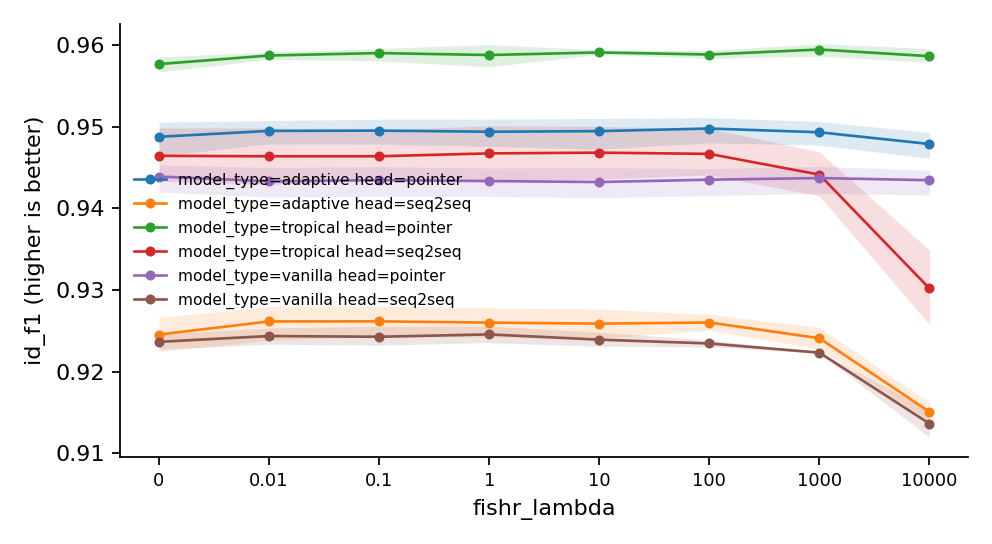
\includegraphics[width=\textwidth]{metric_id_f1.png}
\caption{\texttt{id\_f1} against \texttt{fishr\_lambda}: the mean over seeds with a 95\% bootstrap CI, one line per combination of the other factors.}
\label{fig:id_f1}
\end{figure}

{\small
\begin{longtable}{lllrlrrr}
\caption{\texttt{id\_f1} per cell: mean, 95\% bootstrap CI, SD, seeds, diverged runs.}\label{tab:summary-id_f1}\\
\toprule
\texttt{model\_type} & \texttt{head} & \texttt{fishr\_lambda} & mean & 95\% CI & SD & $n$ & div.\\
\midrule
\endhead
adaptive & pointer & 0 & 0.9487 & [0.946, 0.951] & 0.0028 & 5 & 0\\
adaptive & pointer & 0.01 & 0.9495 & [0.948, 0.951] & 0.00188 & 5 & 0\\
adaptive & pointer & 0.1 & 0.9495 & [0.948, 0.951] & 0.002 & 5 & 0\\
adaptive & pointer & 1 & 0.9494 & [0.948, 0.951] & 0.0022 & 5 & 0\\
adaptive & pointer & 10 & 0.9494 & [0.947, 0.951] & 0.00248 & 5 & 0\\
adaptive & pointer & 100 & 0.9498 & [0.948, 0.951] & 0.00197 & 5 & 0\\
adaptive & pointer & 1000 & 0.9493 & [0.948, 0.951] & 0.00183 & 5 & 0\\
adaptive & pointer & 1e+04 & 0.9479 & [0.946, 0.949] & 0.00212 & 5 & 0\\
adaptive & seq2seq & 0 & 0.9245 & [0.922, 0.927] & 0.00266 & 5 & 0\\
adaptive & seq2seq & 0.01 & 0.9261 & [0.924, 0.928] & 0.00249 & 5 & 0\\
adaptive & seq2seq & 0.1 & 0.9261 & [0.924, 0.928] & 0.00252 & 5 & 0\\
adaptive & seq2seq & 1 & 0.926 & [0.924, 0.928] & 0.00247 & 5 & 0\\
adaptive & seq2seq & 10 & 0.9259 & [0.924, 0.928] & 0.00244 & 5 & 0\\
adaptive & seq2seq & 100 & 0.926 & [0.925, 0.927] & 0.00133 & 5 & 0\\
adaptive & seq2seq & 1000 & 0.9241 & [0.923, 0.925] & 0.00174 & 5 & 0\\
adaptive & seq2seq & 1e+04 & 0.9151 & [0.914, 0.916] & 0.00148 & 5 & 0\\
tropical & pointer & 0 & 0.9577 & [0.957, 0.959] & 0.00117 & 5 & 0\\
tropical & pointer & 0.01 & 0.9587 & [0.958, 0.959] & $5.89\times10^{-4}$ & 5 & 0\\
tropical & pointer & 0.1 & 0.959 & [0.958, 0.96] & 0.00107 & 5 & 0\\
tropical & pointer & 1 & 0.9588 & [0.957, 0.96] & 0.00173 & 5 & 0\\
tropical & pointer & 10 & 0.9591 & [0.959, 0.959] & $3.48\times10^{-4}$ & 5 & 0\\
tropical & pointer & 100 & 0.9588 & [0.958, 0.959] & $6.53\times10^{-4}$ & 5 & 0\\
tropical & pointer & 1000 & 0.9594 & [0.959, 0.96] & 0.00103 & 5 & 0\\
tropical & pointer & 1e+04 & 0.9586 & [0.958, 0.96] & 0.00112 & 5 & 0\\
tropical & seq2seq & 0 & 0.9464 & [0.943, 0.95] & 0.00418 & 5 & 0\\
tropical & seq2seq & 0.01 & 0.9464 & [0.943, 0.95] & 0.00453 & 5 & 0\\
tropical & seq2seq & 0.1 & 0.9464 & [0.944, 0.95] & 0.00388 & 5 & 0\\
tropical & seq2seq & 1 & 0.9467 & [0.943, 0.95] & 0.00435 & 5 & 0\\
tropical & seq2seq & 10 & 0.9468 & [0.944, 0.95] & 0.00415 & 5 & 0\\
tropical & seq2seq & 100 & 0.9467 & [0.944, 0.95] & 0.00361 & 5 & 0\\
tropical & seq2seq & 1000 & 0.9441 & [0.942, 0.947] & 0.00355 & 5 & 0\\
tropical & seq2seq & 1e+04 & 0.9302 & [0.926, 0.935] & 0.00604 & 5 & 0\\
vanilla & pointer & 0 & 0.9439 & [0.942, 0.945] & 0.00216 & 5 & 0\\
vanilla & pointer & 0.01 & 0.9433 & [0.941, 0.945] & 0.00243 & 5 & 0\\
vanilla & pointer & 0.1 & 0.9434 & [0.941, 0.945] & 0.00228 & 5 & 0\\
vanilla & pointer & 1 & 0.9433 & [0.941, 0.945] & 0.00223 & 5 & 0\\
vanilla & pointer & 10 & 0.9432 & [0.941, 0.945] & 0.00233 & 5 & 0\\
vanilla & pointer & 100 & 0.9435 & [0.942, 0.945] & 0.00217 & 5 & 0\\
vanilla & pointer & 1000 & 0.9437 & [0.942, 0.945] & 0.00219 & 5 & 0\\
vanilla & pointer & 1e+04 & 0.9434 & [0.942, 0.945] & 0.00208 & 5 & 0\\
vanilla & seq2seq & 0 & 0.9236 & [0.923, 0.925] & 0.0012 & 5 & 0\\
vanilla & seq2seq & 0.01 & 0.9244 & [0.923, 0.925] & 0.00134 & 5 & 0\\
vanilla & seq2seq & 0.1 & 0.9243 & [0.923, 0.926] & 0.0014 & 5 & 0\\
vanilla & seq2seq & 1 & 0.9246 & [0.924, 0.926] & 0.00131 & 5 & 0\\
vanilla & seq2seq & 10 & 0.9239 & [0.923, 0.925] & 0.00111 & 5 & 0\\
vanilla & seq2seq & 100 & 0.9234 & [0.923, 0.924] & $5.50\times10^{-4}$ & 5 & 0\\
vanilla & seq2seq & 1000 & 0.9223 & [0.922, 0.922] & $8.82\times10^{-5}$ & 5 & 0\\
vanilla & seq2seq & 1e+04 & 0.9136 & [0.912, 0.915] & 0.00226 & 5 & 0\\
\bottomrule
\end{longtable}
}

{\small
\begin{longtable}{lllrrrl}
\caption{\texttt{id\_f1}: each level of \texttt{fishr\_lambda} against its control (0), within each combination of the other factors. parametric: Dunnett vs control.}\label{tab:control-id_f1}\\
\toprule
\texttt{model\_type} & \texttt{head} & \texttt{fishr\_lambda} & difference & 95\% CI & $p$ & \\
\midrule
\endhead
adaptive & pointer & 0.01 & $7.191\times10^{-4}$ & [-0.00309, 0.00453] & 0.9941 & \\
adaptive & pointer & 0.1 & $7.586\times10^{-4}$ & [-0.00305, 0.00457] & 0.9920 & \\
adaptive & pointer & 1 & $6.173\times10^{-4}$ & [-0.00319, 0.00443] & 0.9976 & \\
adaptive & pointer & 10 & $6.920\times10^{-4}$ & [-0.00312, 0.0045] & 0.9953 & \\
adaptive & pointer & 100 & 0.001012 & [-0.0028, 0.00482] & 0.9624 & \\
adaptive & pointer & 1000 & $5.515\times10^{-4}$ & [-0.00326, 0.00436] & 0.9988 & \\
adaptive & pointer & 1e+04 & $-8.832\times10^{-4}$ & [-0.00469, 0.00293] & 0.9814 & \\
adaptive & seq2seq & 0.01 & 0.001601 & [-0.00224, 0.00544] & 0.7615 & \\
adaptive & seq2seq & 0.1 & 0.001613 & [-0.00223, 0.00545] & 0.7558 & \\
adaptive & seq2seq & 1 & 0.001458 & [-0.00238, 0.0053] & 0.8265 & \\
adaptive & seq2seq & 10 & 0.001335 & [-0.0025, 0.00517] & 0.8756 & \\
adaptive & seq2seq & 100 & 0.001472 & [-0.00237, 0.00531] & 0.8203 & \\
adaptive & seq2seq & 1000 & $-4.503\times10^{-4}$ & [-0.00429, 0.00339] & 0.9997 & \\
adaptive & seq2seq & 1e+04 & -0.009464 & [-0.0133, -0.00563] & $<10^{-4}$ & *\\
tropical & pointer & 0.01 & 0.001051 & [$-7.69\times10^{-4}$, 0.00287] & 0.4551 & \\
tropical & pointer & 0.1 & 0.001346 & [$-4.74\times10^{-4}$, 0.00317] & 0.2195 & \\
tropical & pointer & 1 & 0.001109 & [$-7.11\times10^{-4}$, 0.00293] & 0.4005 & \\
tropical & pointer & 10 & 0.001426 & [$-3.94\times10^{-4}$, 0.00325] & 0.1756 & \\
tropical & pointer & 100 & 0.001172 & [$-6.49\times10^{-4}$, 0.00299] & 0.3455 & \\
tropical & pointer & 1000 & 0.001784 & [$-3.58\times10^{-5}$, 0.0036] & 0.0565 & \\
tropical & pointer & 1e+04 & $9.638\times10^{-4}$ & [$-8.56\times10^{-4}$, 0.00278] & 0.5440 & \\
tropical & seq2seq & 0.01 & $-5.083\times10^{-5}$ & [-0.00765, 0.00755] & 1.0000 & \\
tropical & seq2seq & 0.1 & $-5.135\times10^{-5}$ & [-0.00765, 0.00755] & 1.0000 & \\
tropical & seq2seq & 1 & $2.997\times10^{-4}$ & [-0.0073, 0.0079] & 1.0000 & \\
tropical & seq2seq & 10 & $3.918\times10^{-4}$ & [-0.00721, 0.00799] & 1.0000 & \\
tropical & seq2seq & 100 & $2.377\times10^{-4}$ & [-0.00736, 0.00783] & 1.0000 & \\
tropical & seq2seq & 1000 & -0.0023 & [-0.0099, 0.0053] & 0.9306 & \\
tropical & seq2seq & 1e+04 & -0.01624 & [-0.0238, -0.00865] & $<10^{-4}$ & *\\
vanilla & pointer & 0.01 & $-5.813\times10^{-4}$ & [-0.00449, 0.00332] & 0.9986 & \\
vanilla & pointer & 0.1 & $-4.417\times10^{-4}$ & [-0.00435, 0.00346] & 0.9998 & \\
vanilla & pointer & 1 & $-5.504\times10^{-4}$ & [-0.00446, 0.00336] & 0.9990 & \\
vanilla & pointer & 10 & $-6.712\times10^{-4}$ & [-0.00458, 0.00323] & 0.9966 & \\
vanilla & pointer & 100 & $-3.850\times10^{-4}$ & [-0.00429, 0.00352] & 0.9999 & \\
vanilla & pointer & 1000 & $-1.823\times10^{-4}$ & [-0.00409, 0.00372] & 1.0000 & \\
vanilla & pointer & 1e+04 & $-4.465\times10^{-4}$ & [-0.00435, 0.00346] & 0.9997 & \\
vanilla & seq2seq & 0.01 & $7.106\times10^{-4}$ & [-0.00157, 0.00299] & 0.9208 & \\
vanilla & seq2seq & 0.1 & $6.191\times10^{-4}$ & [-0.00166, 0.0029] & 0.9581 & \\
vanilla & seq2seq & 1 & $9.092\times10^{-4}$ & [-0.00137, 0.00319] & 0.7937 & \\
vanilla & seq2seq & 10 & $2.644\times10^{-4}$ & [-0.00201, 0.00254] & 0.9997 & \\
vanilla & seq2seq & 100 & $-2.002\times10^{-4}$ & [-0.00248, 0.00208] & 1.0000 & \\
vanilla & seq2seq & 1000 & -0.001327 & [-0.00361, $9.52\times10^{-4}$] & 0.4466 & \\
vanilla & seq2seq & 1e+04 & -0.01002 & [-0.0123, -0.00774] & $<10^{-4}$ & *\\
\bottomrule
\end{longtable}
}

{\small
\begin{longtable}{llrrrrr}
\caption{\texttt{id\_f1} against log10 \texttt{fishr\_lambda}: parametric: OLS slope t-test, seed-bootstrap CI, with the Jonckheere--Terpstra ordered-trend $\tau$ and $p$.}\label{tab:trend-id_f1}\\
\toprule
\texttt{model\_type} & \texttt{head} & estimate & 95\% CI & $p$ & JT $\tau$ & JT $p$\\
\midrule
\endhead
adaptive & pointer & $-1.724\times10^{-4}$ & [$-2.09\times10^{-4}$, $-1.34\times10^{-4}$] & 0.3090 & -0.128 & 0.3351\\
adaptive & seq2seq & -0.001332 & [-0.00152, -0.00104] & $<10^{-4}$ & -0.429 & 0.0008\\
tropical & pointer & $2.418\times10^{-5}$ & [$-9.35\times10^{-5}$, $1.65\times10^{-4}$] & 0.7715 & -0.00571 & 0.9768\\
tropical & seq2seq & -0.001898 & [-0.0023, -0.00151] & 0.0006 & -0.356 & 0.0068\\
vanilla & pointer & $3.887\times10^{-5}$ & [$-1.07\times10^{-4}$, $2.22\times10^{-4}$] & 0.8258 & 0.0781 & 0.5567\\
vanilla & seq2seq & -0.001328 & [-0.00145, -0.00121] & $<10^{-4}$ & -0.619 & 0.0002\\
\bottomrule
\end{longtable}
}

{\small
\begin{longtable}{lrrrl}
\caption{\texttt{id\_f1}: paired contrasts by seed, Holm-corrected across the cells. parametric: paired t-test by seed, Holm.}\label{tab:paired-id_f1}\\
\toprule
contrast (within) & difference & 95\% CI & $p$ & \\
\midrule
\endhead
\stackcell{model\_type: tropical - vanilla\\\footnotesize head=pointer fishr\_lambda=0 } & 0.01377 & [0.0106, 0.017] & 0.0013 & *\\
\stackcell{model\_type: tropical - vanilla\\\footnotesize head=pointer fishr\_lambda=0.01 } & 0.01541 & [0.0126, 0.0182] & 0.0013 & *\\
\stackcell{model\_type: tropical - vanilla\\\footnotesize head=pointer fishr\_lambda=0.1 } & 0.01556 & [0.0126, 0.0186] & 0.0013 & *\\
\stackcell{model\_type: tropical - vanilla\\\footnotesize head=pointer fishr\_lambda=1 } & 0.01543 & [0.0113, 0.0195] & 0.0013 & *\\
\stackcell{model\_type: tropical - vanilla\\\footnotesize head=pointer fishr\_lambda=10 } & 0.01587 & [0.0132, 0.0186] & 0.0012 & *\\
\stackcell{model\_type: tropical - vanilla\\\footnotesize head=pointer fishr\_lambda=100 } & 0.01533 & [0.0125, 0.0181] & 0.0013 & *\\
\stackcell{model\_type: tropical - vanilla\\\footnotesize head=pointer fishr\_lambda=1000 } & 0.01574 & [0.0121, 0.0194] & 0.0013 & *\\
\stackcell{model\_type: tropical - vanilla\\\footnotesize head=pointer fishr\_lambda=1e+04 } & 0.01518 & [0.0124, 0.018] & 0.0013 & *\\
\stackcell{model\_type: tropical - vanilla\\\footnotesize head=seq2seq fishr\_lambda=0 } & 0.02277 & [0.0181, 0.0274] & 0.0013 & *\\
\stackcell{model\_type: tropical - vanilla\\\footnotesize head=seq2seq fishr\_lambda=0.01 } & 0.02201 & [0.0176, 0.0265] & 0.0013 & *\\
\stackcell{model\_type: tropical - vanilla\\\footnotesize head=seq2seq fishr\_lambda=0.1 } & 0.0221 & [0.0185, 0.0257] & 0.0012 & *\\
\stackcell{model\_type: tropical - vanilla\\\footnotesize head=seq2seq fishr\_lambda=1 } & 0.02217 & [0.0175, 0.0268] & 0.0013 & *\\
\stackcell{model\_type: tropical - vanilla\\\footnotesize head=seq2seq fishr\_lambda=10 } & 0.0229 & [0.0188, 0.027] & 0.0013 & *\\
\stackcell{model\_type: tropical - vanilla\\\footnotesize head=seq2seq fishr\_lambda=100 } & 0.02321 & [0.0194, 0.0271] & 0.0012 & *\\
\stackcell{model\_type: tropical - vanilla\\\footnotesize head=seq2seq fishr\_lambda=1000 } & 0.0218 & [0.0174, 0.0262] & 0.0013 & *\\
\stackcell{model\_type: tropical - vanilla\\\footnotesize head=seq2seq fishr\_lambda=1e+04 } & 0.01655 & [0.011, 0.0221] & 0.0013 & *\\
\stackcell{model\_type: adaptive - vanilla\\\footnotesize head=pointer fishr\_lambda=0 } & 0.00487 & [0.00392, 0.00581] & 0.0022 & *\\
\stackcell{model\_type: adaptive - vanilla\\\footnotesize head=pointer fishr\_lambda=0.01 } & 0.00617 & [0.00365, 0.00869] & 0.0221 & *\\
\stackcell{model\_type: adaptive - vanilla\\\footnotesize head=pointer fishr\_lambda=0.1 } & 0.00607 & [0.00396, 0.00818] & 0.0133 & *\\
\stackcell{model\_type: adaptive - vanilla\\\footnotesize head=pointer fishr\_lambda=1 } & 0.006037 & [0.00409, 0.00799] & 0.0111 & *\\
\stackcell{model\_type: adaptive - vanilla\\\footnotesize head=pointer fishr\_lambda=10 } & 0.006233 & [0.00434, 0.00813] & 0.0095 & *\\
\stackcell{model\_type: adaptive - vanilla\\\footnotesize head=pointer fishr\_lambda=100 } & 0.006267 & [0.00478, 0.00776] & 0.0044 & *\\
\stackcell{model\_type: adaptive - vanilla\\\footnotesize head=pointer fishr\_lambda=1000 } & 0.005603 & [0.00429, 0.00692] & 0.0044 & *\\
\stackcell{model\_type: adaptive - vanilla\\\footnotesize head=pointer fishr\_lambda=1e+04 } & 0.004433 & [0.00312, 0.00574] & 0.0093 & *\\
\stackcell{model\_type: adaptive - vanilla\\\footnotesize head=seq2seq fishr\_lambda=0 } & $8.940\times10^{-4}$ & [-0.00138, 0.00317] & 0.3373 & \\
\stackcell{model\_type: adaptive - vanilla\\\footnotesize head=seq2seq fishr\_lambda=0.01 } & 0.001784 & [$-1.39\times10^{-4}$, 0.00371] & 0.2891 & \\
\stackcell{model\_type: adaptive - vanilla\\\footnotesize head=seq2seq fishr\_lambda=0.1 } & 0.001888 & [$-1.01\times10^{-4}$, 0.00388] & 0.2891 & \\
\stackcell{model\_type: adaptive - vanilla\\\footnotesize head=seq2seq fishr\_lambda=1 } & 0.001443 & [$-6.00\times10^{-4}$, 0.00348] & 0.2891 & \\
\stackcell{model\_type: adaptive - vanilla\\\footnotesize head=seq2seq fishr\_lambda=10 } & 0.001964 & [$3.00\times10^{-5}$, 0.0039] & 0.2871 & \\
\stackcell{model\_type: adaptive - vanilla\\\footnotesize head=seq2seq fishr\_lambda=100 } & 0.002566 & [0.00147, 0.00366] & 0.0230 & *\\
\stackcell{model\_type: adaptive - vanilla\\\footnotesize head=seq2seq fishr\_lambda=1000 } & 0.00177 & [$-3.80\times10^{-4}$, 0.00392] & 0.2891 & \\
\stackcell{model\_type: adaptive - vanilla\\\footnotesize head=seq2seq fishr\_lambda=1e+04 } & 0.001447 & [$3.79\times10^{-4}$, 0.00251] & 0.1381 & \\
\stackcell{head: pointer - seq2seq\\\footnotesize model\_type=adaptive fishr\_lambda=0 } & 0.02421 & [0.0212, 0.0272] & 0.0002 & *\\
\stackcell{head: pointer - seq2seq\\\footnotesize model\_type=adaptive fishr\_lambda=0.01 } & 0.02333 & [0.0214, 0.0253] & $<10^{-4}$ & *\\
\stackcell{head: pointer - seq2seq\\\footnotesize model\_type=adaptive fishr\_lambda=0.1 } & 0.02336 & [0.0215, 0.0252] & $<10^{-4}$ & *\\
\stackcell{head: pointer - seq2seq\\\footnotesize model\_type=adaptive fishr\_lambda=1 } & 0.02337 & [0.0218, 0.025] & $<10^{-4}$ & *\\
\stackcell{head: pointer - seq2seq\\\footnotesize model\_type=adaptive fishr\_lambda=10 } & 0.02357 & [0.0218, 0.0254] & $<10^{-4}$ & *\\
\stackcell{head: pointer - seq2seq\\\footnotesize model\_type=adaptive fishr\_lambda=100 } & 0.02375 & [0.0211, 0.0264] & 0.0002 & *\\
\stackcell{head: pointer - seq2seq\\\footnotesize model\_type=adaptive fishr\_lambda=1000 } & 0.02522 & [0.0224, 0.028] & 0.0002 & *\\
\stackcell{head: pointer - seq2seq\\\footnotesize model\_type=adaptive fishr\_lambda=1e+04 } & 0.03279 & [0.0309, 0.0347] & $<10^{-4}$ & *\\
\stackcell{head: pointer - seq2seq\\\footnotesize model\_type=tropical fishr\_lambda=0 } & 0.01124 & [0.00658, 0.0159] & 0.0155 & *\\
\stackcell{head: pointer - seq2seq\\\footnotesize model\_type=tropical fishr\_lambda=0.01 } & 0.01234 & [0.00643, 0.0182] & 0.0155 & *\\
\stackcell{head: pointer - seq2seq\\\footnotesize model\_type=tropical fishr\_lambda=0.1 } & 0.01263 & [0.00723, 0.018] & 0.0155 & *\\
\stackcell{head: pointer - seq2seq\\\footnotesize model\_type=tropical fishr\_lambda=1 } & 0.01205 & [0.00564, 0.0184] & 0.0155 & *\\
\stackcell{head: pointer - seq2seq\\\footnotesize model\_type=tropical fishr\_lambda=10 } & 0.01227 & [0.00687, 0.0177] & 0.0155 & *\\
\stackcell{head: pointer - seq2seq\\\footnotesize model\_type=tropical fishr\_lambda=100 } & 0.01217 & [0.00696, 0.0174] & 0.0155 & *\\
\stackcell{head: pointer - seq2seq\\\footnotesize model\_type=tropical fishr\_lambda=1000 } & 0.01532 & [0.01, 0.0206] & 0.0091 & *\\
\stackcell{head: pointer - seq2seq\\\footnotesize model\_type=tropical fishr\_lambda=1e+04 } & 0.02844 & [0.0204, 0.0365] & 0.0048 & *\\
\stackcell{head: pointer - seq2seq\\\footnotesize model\_type=vanilla fishr\_lambda=0 } & 0.02024 & [0.0179, 0.0225] & 0.0002 & *\\
\stackcell{head: pointer - seq2seq\\\footnotesize model\_type=vanilla fishr\_lambda=0.01 } & 0.01895 & [0.0167, 0.0212] & 0.0002 & *\\
\stackcell{head: pointer - seq2seq\\\footnotesize model\_type=vanilla fishr\_lambda=0.1 } & 0.01918 & [0.0174, 0.021] & 0.0001 & *\\
\stackcell{head: pointer - seq2seq\\\footnotesize model\_type=vanilla fishr\_lambda=1 } & 0.01878 & [0.0167, 0.0208] & 0.0002 & *\\
\stackcell{head: pointer - seq2seq\\\footnotesize model\_type=vanilla fishr\_lambda=10 } & 0.0193 & [0.0173, 0.0213] & 0.0002 & *\\
\stackcell{head: pointer - seq2seq\\\footnotesize model\_type=vanilla fishr\_lambda=100 } & 0.02005 & [0.0177, 0.0225] & 0.0002 & *\\
\stackcell{head: pointer - seq2seq\\\footnotesize model\_type=vanilla fishr\_lambda=1000 } & 0.02138 & [0.0187, 0.0241] & 0.0002 & *\\
\stackcell{head: pointer - seq2seq\\\footnotesize model\_type=vanilla fishr\_lambda=1e+04 } & 0.02981 & [0.0286, 0.031] & $<10^{-4}$ & *\\
\bottomrule
\end{longtable}
}

\subsection{\texttt{id\_exact}}
\begin{figure}[tbp]
\centering
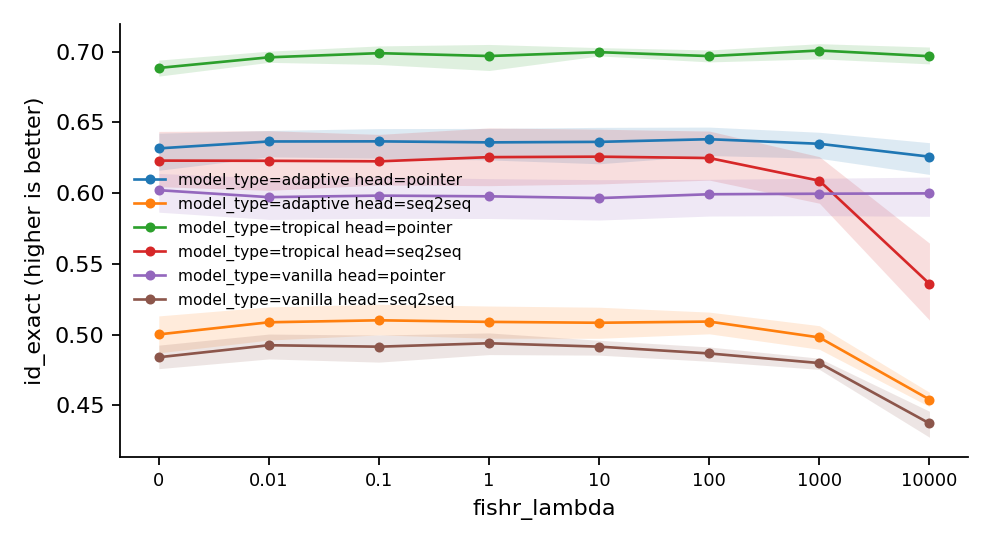
\includegraphics[width=\textwidth]{metric_id_exact.png}
\caption{\texttt{id\_exact} against \texttt{fishr\_lambda}: the mean over seeds with a 95\% bootstrap CI, one line per combination of the other factors.}
\label{fig:id_exact}
\end{figure}

{\small
\begin{longtable}{lllrlrrr}
\caption{\texttt{id\_exact} per cell: mean, 95\% bootstrap CI, SD, seeds, diverged runs.}\label{tab:summary-id_exact}\\
\toprule
\texttt{model\_type} & \texttt{head} & \texttt{fishr\_lambda} & mean & 95\% CI & SD & $n$ & div.\\
\midrule
\endhead
adaptive & pointer & 0 & 0.6317 & [0.616, 0.642] & 0.018 & 5 & 0\\
adaptive & pointer & 0.01 & 0.6365 & [0.626, 0.644] & 0.0125 & 5 & 0\\
adaptive & pointer & 0.1 & 0.6366 & [0.625, 0.646] & 0.0136 & 5 & 0\\
adaptive & pointer & 1 & 0.6359 & [0.623, 0.646] & 0.0144 & 5 & 0\\
adaptive & pointer & 10 & 0.6363 & [0.621, 0.646] & 0.0172 & 5 & 0\\
adaptive & pointer & 100 & 0.6381 & [0.627, 0.647] & 0.0127 & 5 & 0\\
adaptive & pointer & 1000 & 0.6349 & [0.625, 0.643] & 0.0115 & 5 & 0\\
adaptive & pointer & 1e+04 & 0.6258 & [0.613, 0.636] & 0.0146 & 5 & 0\\
adaptive & seq2seq & 0 & 0.5002 & [0.487, 0.513] & 0.0167 & 5 & 0\\
adaptive & seq2seq & 0.01 & 0.5088 & [0.496, 0.52] & 0.0145 & 5 & 0\\
adaptive & seq2seq & 0.1 & 0.5102 & [0.5, 0.522] & 0.0148 & 5 & 0\\
adaptive & seq2seq & 1 & 0.5091 & [0.498, 0.52] & 0.0154 & 5 & 0\\
adaptive & seq2seq & 10 & 0.5084 & [0.497, 0.519] & 0.0146 & 5 & 0\\
adaptive & seq2seq & 100 & 0.5093 & [0.501, 0.516] & 0.01 & 5 & 0\\
adaptive & seq2seq & 1000 & 0.4981 & [0.49, 0.506] & 0.0108 & 5 & 0\\
adaptive & seq2seq & 1e+04 & 0.4542 & [0.449, 0.459] & 0.00652 & 5 & 0\\
tropical & pointer & 0 & 0.6885 & [0.683, 0.694] & 0.00741 & 5 & 0\\
tropical & pointer & 0.01 & 0.696 & [0.692, 0.7] & 0.00502 & 5 & 0\\
tropical & pointer & 0.1 & 0.6989 & [0.691, 0.704] & 0.00894 & 5 & 0\\
tropical & pointer & 1 & 0.6969 & [0.687, 0.705] & 0.0119 & 5 & 0\\
tropical & pointer & 10 & 0.6996 & [0.697, 0.703] & 0.00374 & 5 & 0\\
tropical & pointer & 100 & 0.6969 & [0.693, 0.701] & 0.0057 & 5 & 0\\
tropical & pointer & 1000 & 0.7008 & [0.695, 0.706] & 0.00694 & 5 & 0\\
tropical & pointer & 1e+04 & 0.6968 & [0.691, 0.703] & 0.00744 & 5 & 0\\
tropical & seq2seq & 0 & 0.623 & [0.605, 0.644] & 0.0248 & 5 & 0\\
tropical & seq2seq & 0.01 & 0.6229 & [0.602, 0.644] & 0.0274 & 5 & 0\\
tropical & seq2seq & 0.1 & 0.6225 & [0.606, 0.642] & 0.0236 & 5 & 0\\
tropical & seq2seq & 1 & 0.6255 & [0.605, 0.646] & 0.0268 & 5 & 0\\
tropical & seq2seq & 10 & 0.6258 & [0.607, 0.645] & 0.025 & 5 & 0\\
tropical & seq2seq & 100 & 0.6248 & [0.609, 0.644] & 0.0219 & 5 & 0\\
tropical & seq2seq & 1000 & 0.6088 & [0.593, 0.626] & 0.0217 & 5 & 0\\
tropical & seq2seq & 1e+04 & 0.536 & [0.51, 0.565] & 0.0349 & 5 & 0\\
vanilla & pointer & 0 & 0.6021 & [0.587, 0.614] & 0.0177 & 5 & 0\\
vanilla & pointer & 0.01 & 0.5972 & [0.581, 0.611] & 0.0192 & 5 & 0\\
vanilla & pointer & 0.1 & 0.5983 & [0.582, 0.612] & 0.0182 & 5 & 0\\
vanilla & pointer & 1 & 0.5978 & [0.582, 0.61] & 0.0179 & 5 & 0\\
vanilla & pointer & 10 & 0.5965 & [0.581, 0.61] & 0.0184 & 5 & 0\\
vanilla & pointer & 100 & 0.5992 & [0.584, 0.61] & 0.0173 & 5 & 0\\
vanilla & pointer & 1000 & 0.5996 & [0.584, 0.611] & 0.0179 & 5 & 0\\
vanilla & pointer & 1e+04 & 0.5999 & [0.584, 0.611] & 0.019 & 5 & 0\\
vanilla & seq2seq & 0 & 0.4841 & [0.476, 0.493] & 0.0108 & 5 & 0\\
vanilla & seq2seq & 0.01 & 0.4926 & [0.483, 0.5] & 0.0112 & 5 & 0\\
vanilla & seq2seq & 0.1 & 0.4915 & [0.481, 0.5] & 0.0123 & 5 & 0\\
vanilla & seq2seq & 1 & 0.494 & [0.486, 0.501] & 0.0107 & 5 & 0\\
vanilla & seq2seq & 10 & 0.4916 & [0.486, 0.496] & 0.00685 & 5 & 0\\
vanilla & seq2seq & 100 & 0.4868 & [0.481, 0.491] & 0.0068 & 5 & 0\\
vanilla & seq2seq & 1000 & 0.48 & [0.475, 0.483] & 0.00519 & 5 & 0\\
vanilla & seq2seq & 1e+04 & 0.4373 & [0.428, 0.446] & 0.0117 & 5 & 0\\
\bottomrule
\end{longtable}
}

{\small
\begin{longtable}{lllrrrl}
\caption{\texttt{id\_exact}: each level of \texttt{fishr\_lambda} against its control (0), within each combination of the other factors. parametric: Dunnett vs control.}\label{tab:control-id_exact}\\
\toprule
\texttt{model\_type} & \texttt{head} & \texttt{fishr\_lambda} & difference & 95\% CI & $p$ & \\
\midrule
\endhead
adaptive & pointer & 0.01 & 0.00488 & [-0.0204, 0.0301] & 0.9932 & \\
adaptive & pointer & 0.1 & 0.00496 & [-0.0203, 0.0302] & 0.9926 & \\
adaptive & pointer & 1 & 0.00424 & [-0.021, 0.0295] & 0.9970 & \\
adaptive & pointer & 10 & 0.0046 & [-0.0207, 0.0299] & 0.9952 & \\
adaptive & pointer & 100 & 0.00648 & [-0.0188, 0.0317] & 0.9684 & \\
adaptive & pointer & 1000 & 0.00324 & [-0.022, 0.0285] & 0.9994 & \\
adaptive & pointer & 1e+04 & -0.00586 & [-0.0311, 0.0194] & 0.9813 & \\
adaptive & seq2seq & 0.01 & 0.00856 & [-0.0147, 0.0318] & 0.8455 & \\
adaptive & seq2seq & 0.1 & 0.00996 & [-0.0133, 0.0332] & 0.7410 & \\
adaptive & seq2seq & 1 & 0.00884 & [-0.0144, 0.0321] & 0.8262 & \\
adaptive & seq2seq & 10 & 0.00822 & [-0.015, 0.0315] & 0.8676 & \\
adaptive & seq2seq & 100 & 0.00906 & [-0.0142, 0.0323] & 0.8103 & \\
adaptive & seq2seq & 1000 & -0.00216 & [-0.0254, 0.0211] & 0.9999 & \\
adaptive & seq2seq & 1e+04 & -0.04602 & [-0.0693, -0.0228] & $<10^{-4}$ & *\\
tropical & pointer & 0.01 & 0.0075 & [-0.00563, 0.0206] & 0.4660 & \\
tropical & pointer & 0.1 & 0.01044 & [-0.00269, 0.0236] & 0.1647 & \\
tropical & pointer & 1 & 0.00842 & [-0.00471, 0.0215] & 0.3488 & \\
tropical & pointer & 10 & 0.01114 & [-0.00199, 0.0243] & 0.1232 & \\
tropical & pointer & 100 & 0.00838 & [-0.00475, 0.0215] & 0.3535 & \\
tropical & pointer & 1000 & 0.01232 & [$-8.06\times10^{-4}$, 0.0254] & 0.0730 & \\
tropical & pointer & 1e+04 & 0.00828 & [-0.00485, 0.0214] & 0.3653 & \\
tropical & seq2seq & 0.01 & $-1.400\times10^{-4}$ & [-0.0457, 0.0454] & 1.0000 & \\
tropical & seq2seq & 0.1 & $-5.000\times10^{-4}$ & [-0.0461, 0.0451] & 1.0000 & \\
tropical & seq2seq & 1 & 0.00244 & [-0.0431, 0.048] & 1.0000 & \\
tropical & seq2seq & 10 & 0.00278 & [-0.0428, 0.0483] & 1.0000 & \\
tropical & seq2seq & 100 & 0.00182 & [-0.0437, 0.0474] & 1.0000 & \\
tropical & seq2seq & 1000 & -0.0142 & [-0.0598, 0.0314] & 0.9210 & \\
tropical & seq2seq & 1e+04 & -0.08704 & [-0.133, -0.0415] & $<10^{-4}$ & *\\
vanilla & pointer & 0.01 & -0.00492 & [-0.0367, 0.0269] & 0.9982 & \\
vanilla & pointer & 0.1 & -0.00384 & [-0.0356, 0.0279] & 0.9996 & \\
vanilla & pointer & 1 & -0.00434 & [-0.0361, 0.0274] & 0.9992 & \\
vanilla & pointer & 10 & -0.00558 & [-0.0374, 0.0262] & 0.9961 & \\
vanilla & pointer & 100 & -0.00288 & [-0.0347, 0.0289] & 0.9999 & \\
vanilla & pointer & 1000 & -0.0025 & [-0.0343, 0.0293] & 1.0000 & \\
vanilla & pointer & 1e+04 & -0.00226 & [-0.034, 0.0295] & 1.0000 & \\
vanilla & seq2seq & 0.01 & 0.00848 & [-0.00861, 0.0256] & 0.6088 & \\
vanilla & seq2seq & 0.1 & 0.00746 & [-0.00963, 0.0246] & 0.7251 & \\
vanilla & seq2seq & 1 & 0.00988 & [-0.00721, 0.027] & 0.4540 & \\
vanilla & seq2seq & 10 & 0.00748 & [-0.00961, 0.0246] & 0.7227 & \\
vanilla & seq2seq & 100 & 0.00268 & [-0.0144, 0.0198] & 0.9980 & \\
vanilla & seq2seq & 1000 & -0.00412 & [-0.0212, 0.013] & 0.9771 & \\
vanilla & seq2seq & 1e+04 & -0.04674 & [-0.0638, -0.0296] & $<10^{-4}$ & *\\
\bottomrule
\end{longtable}
}

{\small
\begin{longtable}{llrrrrr}
\caption{\texttt{id\_exact} against log10 \texttt{fishr\_lambda}: parametric: OLS slope t-test, seed-bootstrap CI, with the Jonckheere--Terpstra ordered-trend $\tau$ and $p$.}\label{tab:trend-id_exact}\\
\toprule
\texttt{model\_type} & \texttt{head} & estimate & 95\% CI & $p$ & JT $\tau$ & JT $p$\\
\midrule
\endhead
adaptive & pointer & -0.001194 & [-0.0014, -0.00105] & 0.2904 & -0.149 & 0.2559\\
adaptive & seq2seq & -0.006706 & [-0.00785, -0.00497] & 0.0001 & -0.383 & 0.0036\\
tropical & pointer & $2.164\times10^{-4}$ & [$-5.19\times10^{-4}$, 0.00104] & 0.7218 & -0.00381 & 0.9872\\
tropical & seq2seq & -0.01031 & [-0.0126, -0.00797] & 0.0009 & -0.354 & 0.0066\\
vanilla & pointer & $4.329\times10^{-4}$ & [$-8.17\times10^{-4}$, 0.002] & 0.7630 & 0.109 & 0.4117\\
vanilla & seq2seq & -0.007001 & [-0.0076, -0.00596] & $<10^{-4}$ & -0.566 & 0.0002\\
\bottomrule
\end{longtable}
}

{\small
\begin{longtable}{lrrrl}
\caption{\texttt{id\_exact}: paired contrasts by seed, Holm-corrected across the cells. parametric: paired t-test by seed, Holm.}\label{tab:paired-id_exact}\\
\toprule
contrast (within) & difference & 95\% CI & $p$ & \\
\midrule
\endhead
\stackcell{model\_type: tropical - vanilla\\\footnotesize head=pointer fishr\_lambda=0 } & 0.08638 & [0.0612, 0.112] & 0.0029 & *\\
\stackcell{model\_type: tropical - vanilla\\\footnotesize head=pointer fishr\_lambda=0.01 } & 0.0988 & [0.0766, 0.121] & 0.0029 & *\\
\stackcell{model\_type: tropical - vanilla\\\footnotesize head=pointer fishr\_lambda=0.1 } & 0.1007 & [0.0755, 0.126] & 0.0029 & *\\
\stackcell{model\_type: tropical - vanilla\\\footnotesize head=pointer fishr\_lambda=1 } & 0.09914 & [0.0681, 0.13] & 0.0029 & *\\
\stackcell{model\_type: tropical - vanilla\\\footnotesize head=pointer fishr\_lambda=10 } & 0.1031 & [0.0811, 0.125] & 0.0028 & *\\
\stackcell{model\_type: tropical - vanilla\\\footnotesize head=pointer fishr\_lambda=100 } & 0.09764 & [0.0759, 0.119] & 0.0029 & *\\
\stackcell{model\_type: tropical - vanilla\\\footnotesize head=pointer fishr\_lambda=1000 } & 0.1012 & [0.073, 0.129] & 0.0029 & *\\
\stackcell{model\_type: tropical - vanilla\\\footnotesize head=pointer fishr\_lambda=1e+04 } & 0.09692 & [0.0715, 0.122] & 0.0029 & *\\
\stackcell{model\_type: tropical - vanilla\\\footnotesize head=seq2seq fishr\_lambda=0 } & 0.1389 & [0.105, 0.172] & 0.0029 & *\\
\stackcell{model\_type: tropical - vanilla\\\footnotesize head=seq2seq fishr\_lambda=0.01 } & 0.1303 & [0.1, 0.161] & 0.0029 & *\\
\stackcell{model\_type: tropical - vanilla\\\footnotesize head=seq2seq fishr\_lambda=0.1 } & 0.131 & [0.105, 0.157] & 0.0024 & *\\
\stackcell{model\_type: tropical - vanilla\\\footnotesize head=seq2seq fishr\_lambda=1 } & 0.1315 & [0.1, 0.163] & 0.0029 & *\\
\stackcell{model\_type: tropical - vanilla\\\footnotesize head=seq2seq fishr\_lambda=10 } & 0.1342 & [0.105, 0.164] & 0.0029 & *\\
\stackcell{model\_type: tropical - vanilla\\\footnotesize head=seq2seq fishr\_lambda=100 } & 0.1381 & [0.114, 0.162] & 0.0014 & *\\
\stackcell{model\_type: tropical - vanilla\\\footnotesize head=seq2seq fishr\_lambda=1000 } & 0.1289 & [0.101, 0.157] & 0.0029 & *\\
\stackcell{model\_type: tropical - vanilla\\\footnotesize head=seq2seq fishr\_lambda=1e+04 } & 0.09864 & [0.0646, 0.133] & 0.0029 & *\\
\stackcell{model\_type: adaptive - vanilla\\\footnotesize head=pointer fishr\_lambda=0 } & 0.02954 & [0.0258, 0.0332] & 0.0004 & *\\
\stackcell{model\_type: adaptive - vanilla\\\footnotesize head=pointer fishr\_lambda=0.01 } & 0.03934 & [0.0222, 0.0564] & 0.0246 & *\\
\stackcell{model\_type: adaptive - vanilla\\\footnotesize head=pointer fishr\_lambda=0.1 } & 0.03834 & [0.0234, 0.0533] & 0.0192 & *\\
\stackcell{model\_type: adaptive - vanilla\\\footnotesize head=pointer fishr\_lambda=1 } & 0.03812 & [0.0252, 0.051] & 0.0133 & *\\
\stackcell{model\_type: adaptive - vanilla\\\footnotesize head=pointer fishr\_lambda=10 } & 0.03972 & [0.0266, 0.0528] & 0.0130 & *\\
\stackcell{model\_type: adaptive - vanilla\\\footnotesize head=pointer fishr\_lambda=100 } & 0.0389 & [0.0279, 0.0499] & 0.0091 & *\\
\stackcell{model\_type: adaptive - vanilla\\\footnotesize head=pointer fishr\_lambda=1000 } & 0.03528 & [0.0243, 0.0462] & 0.0112 & *\\
\stackcell{model\_type: adaptive - vanilla\\\footnotesize head=pointer fishr\_lambda=1e+04 } & 0.02594 & [0.016, 0.0359] & 0.0192 & *\\
\stackcell{model\_type: adaptive - vanilla\\\footnotesize head=seq2seq fishr\_lambda=0 } & 0.01614 & [-0.00418, 0.0365] & 0.0921 & \\
\stackcell{model\_type: adaptive - vanilla\\\footnotesize head=seq2seq fishr\_lambda=0.01 } & 0.01622 & [0.00839, 0.024] & 0.0317 & *\\
\stackcell{model\_type: adaptive - vanilla\\\footnotesize head=seq2seq fishr\_lambda=0.1 } & 0.01864 & [0.00916, 0.0281] & 0.0329 & *\\
\stackcell{model\_type: adaptive - vanilla\\\footnotesize head=seq2seq fishr\_lambda=1 } & 0.0151 & [0.00456, 0.0256] & 0.0647 & \\
\stackcell{model\_type: adaptive - vanilla\\\footnotesize head=seq2seq fishr\_lambda=10 } & 0.01688 & [0.00471, 0.0291] & 0.0647 & \\
\stackcell{model\_type: adaptive - vanilla\\\footnotesize head=seq2seq fishr\_lambda=100 } & 0.02252 & [0.0161, 0.0289] & 0.0091 & *\\
\stackcell{model\_type: adaptive - vanilla\\\footnotesize head=seq2seq fishr\_lambda=1000 } & 0.0181 & [0.00553, 0.0307] & 0.0647 & \\
\stackcell{model\_type: adaptive - vanilla\\\footnotesize head=seq2seq fishr\_lambda=1e+04 } & 0.01686 & [0.00792, 0.0258] & 0.0329 & *\\
\stackcell{head: pointer - seq2seq\\\footnotesize model\_type=adaptive fishr\_lambda=0 } & 0.1314 & [0.111, 0.152] & 0.0009 & *\\
\stackcell{head: pointer - seq2seq\\\footnotesize model\_type=adaptive fishr\_lambda=0.01 } & 0.1278 & [0.115, 0.14] & 0.0002 & *\\
\stackcell{head: pointer - seq2seq\\\footnotesize model\_type=adaptive fishr\_lambda=0.1 } & 0.1264 & [0.115, 0.138] & 0.0001 & *\\
\stackcell{head: pointer - seq2seq\\\footnotesize model\_type=adaptive fishr\_lambda=1 } & 0.1268 & [0.116, 0.138] & 0.0001 & *\\
\stackcell{head: pointer - seq2seq\\\footnotesize model\_type=adaptive fishr\_lambda=10 } & 0.1278 & [0.116, 0.14] & 0.0002 & *\\
\stackcell{head: pointer - seq2seq\\\footnotesize model\_type=adaptive fishr\_lambda=100 } & 0.1289 & [0.109, 0.149] & 0.0008 & *\\
\stackcell{head: pointer - seq2seq\\\footnotesize model\_type=adaptive fishr\_lambda=1000 } & 0.1368 & [0.122, 0.151] & 0.0002 & *\\
\stackcell{head: pointer - seq2seq\\\footnotesize model\_type=adaptive fishr\_lambda=1e+04 } & 0.1716 & [0.156, 0.187] & 0.0001 & *\\
\stackcell{head: pointer - seq2seq\\\footnotesize model\_type=tropical fishr\_lambda=0 } & 0.06548 & [0.0367, 0.0943] & 0.0193 & *\\
\stackcell{head: pointer - seq2seq\\\footnotesize model\_type=tropical fishr\_lambda=0.01 } & 0.07312 & [0.0348, 0.111] & 0.0193 & *\\
\stackcell{head: pointer - seq2seq\\\footnotesize model\_type=tropical fishr\_lambda=0.1 } & 0.07642 & [0.04, 0.113] & 0.0193 & *\\
\stackcell{head: pointer - seq2seq\\\footnotesize model\_type=tropical fishr\_lambda=1 } & 0.07146 & [0.0294, 0.113] & 0.0193 & *\\
\stackcell{head: pointer - seq2seq\\\footnotesize model\_type=tropical fishr\_lambda=10 } & 0.07384 & [0.0395, 0.108] & 0.0193 & *\\
\stackcell{head: pointer - seq2seq\\\footnotesize model\_type=tropical fishr\_lambda=100 } & 0.07204 & [0.0388, 0.105] & 0.0193 & *\\
\stackcell{head: pointer - seq2seq\\\footnotesize model\_type=tropical fishr\_lambda=1000 } & 0.092 & [0.058, 0.126] & 0.0117 & *\\
\stackcell{head: pointer - seq2seq\\\footnotesize model\_type=tropical fishr\_lambda=1e+04 } & 0.1608 & [0.114, 0.208] & 0.0055 & *\\
\stackcell{head: pointer - seq2seq\\\footnotesize model\_type=vanilla fishr\_lambda=0 } & 0.118 & [0.0973, 0.139] & 0.0010 & *\\
\stackcell{head: pointer - seq2seq\\\footnotesize model\_type=vanilla fishr\_lambda=0.01 } & 0.1046 & [0.0881, 0.121] & 0.0009 & *\\
\stackcell{head: pointer - seq2seq\\\footnotesize model\_type=vanilla fishr\_lambda=0.1 } & 0.1067 & [0.0933, 0.12] & 0.0004 & *\\
\stackcell{head: pointer - seq2seq\\\footnotesize model\_type=vanilla fishr\_lambda=1 } & 0.1038 & [0.0895, 0.118] & 0.0006 & *\\
\stackcell{head: pointer - seq2seq\\\footnotesize model\_type=vanilla fishr\_lambda=10 } & 0.105 & [0.0875, 0.122] & 0.0009 & *\\
\stackcell{head: pointer - seq2seq\\\footnotesize model\_type=vanilla fishr\_lambda=100 } & 0.1125 & [0.0904, 0.135] & 0.0015 & *\\
\stackcell{head: pointer - seq2seq\\\footnotesize model\_type=vanilla fishr\_lambda=1000 } & 0.1197 & [0.0946, 0.145] & 0.0017 & *\\
\stackcell{head: pointer - seq2seq\\\footnotesize model\_type=vanilla fishr\_lambda=1e+04 } & 0.1625 & [0.152, 0.173] & $<10^{-4}$ & *\\
\bottomrule
\end{longtable}
}


\section{Curves}
\begin{figure}[tbp]
\centering
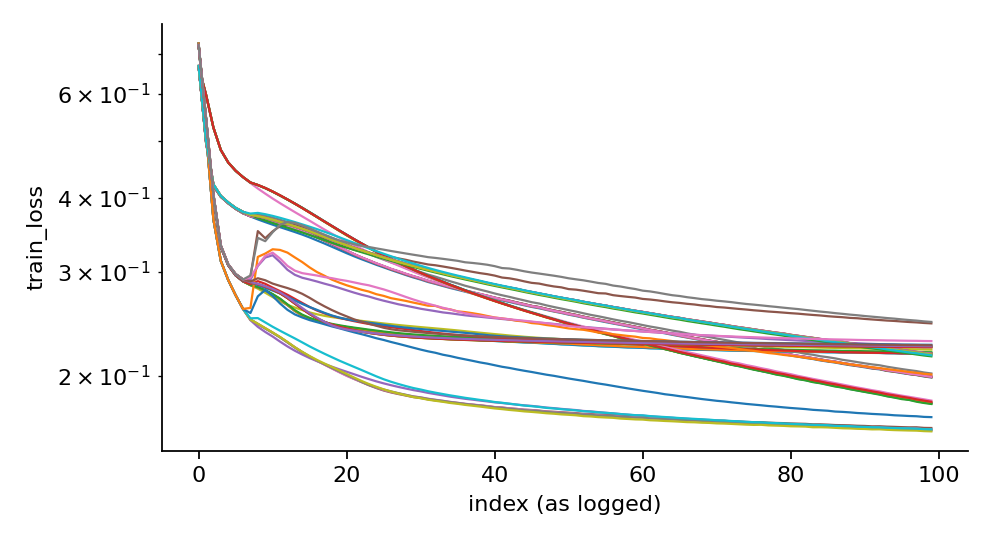
\includegraphics[width=\textwidth]{curve_train_loss.png}
\caption{\texttt{train\_loss}, the mean over seeds per cell.}
\label{fig:curve-1}
\end{figure}
\begin{figure}[tbp]
\centering
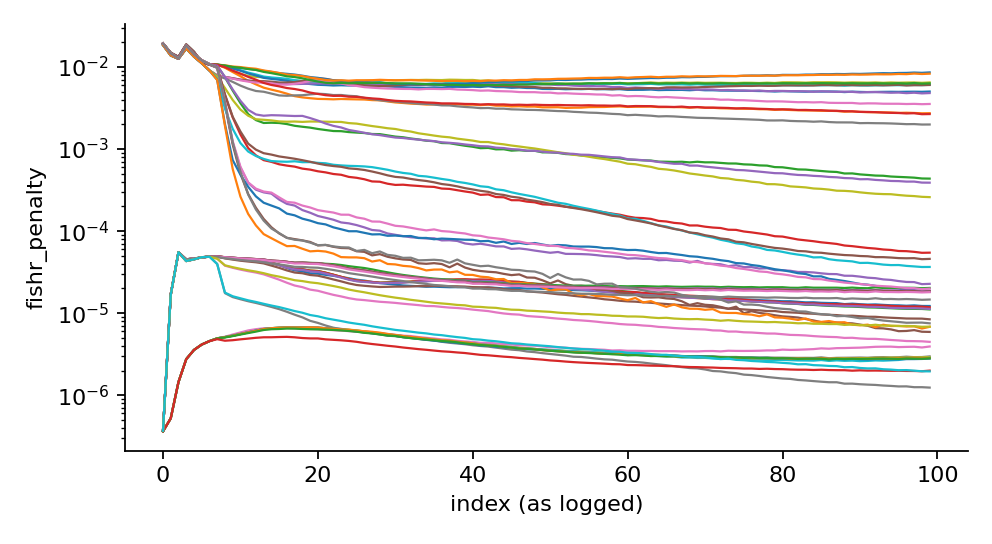
\includegraphics[width=\textwidth]{curve_fishr_penalty.png}
\caption{\texttt{fishr\_penalty}, the mean over seeds per cell.}
\label{fig:curve-2}
\end{figure}
\begin{figure}[tbp]
\centering
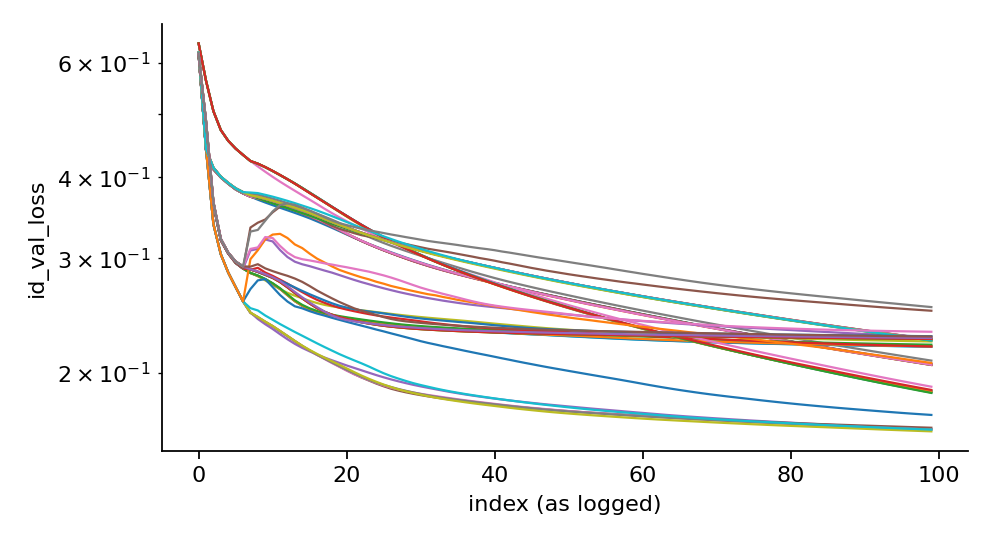
\includegraphics[width=\textwidth]{curve_id_val_loss.png}
\caption{\texttt{id\_val\_loss}, the mean over seeds per cell.}
\label{fig:curve-3}
\end{figure}

\section{Configuration}
The base configuration every run shares (frozen hash \texttt{3b4ea5b21c9e}); factor levels are in \autoref{tab:summary-ood_len_f1}.
{\footnotesize
\begin{verbatim}
task:
  name: FractionalKnapsackDataset
  value_range:
  - 1
  - 10
  target_range:
  - 10
  - 20
  weight_range:
  - 1
  - 10
  adversarial_range:
  - 10
  - 30
  noise_prob: 0.0
data:
  train_lengths:
  - 4
  - 5
  - 6
  - 7
  - 8
  ood_lengths:
  - 12
  - 16
  - 64
  ood_value_range:
  - 11
  - 21
  ood_noise_range:
  - 1
  - 5
  ood_noise_prob: 0.5
  n_per_length: 20000
  n_eval_per_length: 2000
  curve_eval_limit: 256
model:
  d_model: 64
  n_heads: 2
  num_layers: 1
  dropout: 0.0
  tropical_impl: legacy
optim:
  lr: 0.0001
  epochs: 100
  batch_size: 100
  eval_batch_size: 256
fishr:
  ema: 0.95
  anneal_iters: 1500
  reset_optimizer: true
\end{verbatim}
}
Store: \texttt{campaigns/tropical/FractionalKnapsack/results}.
\end{document}